\documentclass[a4paper]{report}

%====================== PACKAGES ======================

\usepackage[french]{babel}
\usepackage[utf8x]{inputenc}
%pour gérer les positionnement d'images
\usepackage{float}
\usepackage{amsmath}
\usepackage{graphicx}
\usepackage[colorinlistoftodos]{todonotes}
\usepackage{url}
\usepackage{titlesec, blindtext, color}
\titleformat{\chapter}{\normalfont\LARGE\bfseries}{\thechapter}{1em}{}
\titlespacing*{\chapter}{0pt}{3.5ex plus 1ex minus .2ex}{2.3ex plus .2ex}
%pour les informations sur un document compilé en PDF et les liens externes / internes
\usepackage{hyperref}
%pour la mise en page des tableaux
\usepackage{array}
\usepackage{tabularx}
%pour utiliser \floatbarrier
%\usepackage{placeins}
%\usepackage{floatrow}
%espacement entre les lignes
\usepackage{setspace}
%modifier la mise en page de l'abstract
\usepackage{abstract}
%police et mise en page (marges) du document
\usepackage[T1]{fontenc}
\usepackage[top=2cm, bottom=2cm, left=2cm, right=2cm]{geometry}
%Pour les galerie d'images
\usepackage{subfig}
\usepackage{tikz}
\usetikzlibrary{shapes,arrows, positioning}
\usepackage{todonotes}
\usepackage[ruled,vlined]{algorithm2e}
\usepackage{appendix}

\newtheorem{definition}{Définition}

%====================== INFORMATION ET REGLES ======================

%rajouter les numérotation pour les \paragraphe et \subparagraphe
\setcounter{secnumdepth}{4}
\setcounter{tocdepth}{4}

\hypersetup{							% Information sur le document
pdfauthor = {Baptiste Mounier},			% Auteurs
pdftitle = {Production de graphes médians pour la phylogénie},			% Titre du document
pdfsubject = {Rapport de stage},		% Sujet
pdfkeywords = {Treillis, Médian,Graphe, Phylogénie},	% Mots-clefs
pdfstartview={FitH}}					% ajuste la page à la largueur de l'écran
%pdfcreator = {MikTeX},% Logiciel qui a crée le document
%pdfproducer = {}} % Société avec produit le logiciel

% tikz rules
\tikzstyle{bnode} = [circle, fill, draw, inner sep = 2pt]
\tikzstyle{wnode} = [circle, draw, inner sep = 2pt]
\tikzstyle{line} = [draw]
\tikzstyle{block2} = [rectangle, draw, text width = 5em, text centered, minimum height = 3em]
\tikzstyle{decision} = [diamond, draw, fill = green!20, text width = 6em, text badly centered, inner sep = 0pt]
\tikzstyle{block} = [rectangle, draw, fill = blue!20, text width = 6em, text centered, rounded corners, minimum height = 3em]
\tikzstyle{algorithm} = [rectangle, draw, fill = green!20, text width = 6em, text centered, rounded corners, minimum height = 3em]
\tikzstyle{inout} = [rectangle, draw, fill = red!20, text width = 6em, text centered, minimum height = 3em]
\tikzstyle{cloud} = [ellipse, draw, fill = red!20, minimum height=2em]
\tikzstyle{line2} = [draw, -latex']
\tikzstyle{line3} = [draw, dashed, -latex']
\tikzstyle{line4} = [draw, dotted, -latex']
\tikzstyle{my below of} = [below=of #1.south]
\tikzstyle{my right of} = [right=of #1.east]
\tikzstyle{my left of} = [left=of #1.west]
\tikzstyle{my above of} = [above=of #1.north]

%======================== DEBUT DU DOCUMENT ========================

\begin{document}

%régler l'espacement entre les lignes
\newcommand{\HRule}{\rule{\linewidth}{0.5mm}}

%page de garde
\begin{titlepage}
\begin{center}

% Upper part of the page. The '~' is needed because only works if a paragraph has started.
\begin{minipage}{0.4\textwidth}
\begin{flushleft}
\includegraphics[width=0.75\textwidth]{title/logo_UL}~\\[1cm]
\end{flushleft}
\end{minipage}
\begin{minipage}{0.4\textwidth}
\begin{flushright}

\includegraphics[width=0.75\textwidth]{title/logo_inria}~\\[1cm]
\end{flushright}
\end{minipage}

\textsc{\Large }\\[3cm]

\textsc{\LARGE UFR Mathématiques et Informatique\bigbreak LORIA}\\[1.5cm]
\textsc{\LARGE Master 2 Sciences Cognitives et Médias Numériques}\\[1.5cm]

% Title
\HRule \\[0.4cm]

{\huge \bfseries Graphes médians, FCA et phylogénie\\[0.4cm] }

\HRule \\[1.5cm]

% Author and supervisor
\begin{minipage}[t]{0.4\textwidth}
\begin{flushleft} \large
\emph{Étudiant:}\\
Baptiste Mounier\\
\bigbreak
\emph{Encadrants:} \\
Miguel Couceiro\\
Alain Gely\\
Amedeo Napoli\\
\bigbreak
\emph{Référent universitaire:} \\
Christine Bourjot
\end{flushleft}
\end{minipage}
\begin{minipage}[t]{0.4\textwidth}
\begin{flushright} \large
\emph{Jury:}\\
Christine Bourjot\\
Miguel Couceiro\\
Manuel Rebuschi\\
Azim Roussanaly\\
\bigbreak
\emph{Date:}\\
09/04/18 - 08/08/18
\end{flushright}
\end{minipage}

% \vfill

% Bottom of the page
% {\large \today}

\end{center}
\end{titlepage}

%page blanche
\newpage
~
\thispagestyle{empty}

\renewcommand{\abstractnamefont}{\normalfont\Large\bfseries}
%\renewcommand{\abstracttextfont}{\normalfont\Huge}

\begin{abstract}
\hskip7mm

\begin{spacing}{1.3}

L'étude de filiation des espèces, phylogénie est un domaine de recherche utilisant des arbres parcimonieux. Par le passé, H.J. Bandelt \cite{cla2018} a mis en avant l'avantage qu'il y a à gagner à encoder l'ensemble des informations dans un unique graphe médian regroupant l'ensemble de ces arbres en même temps. Puis cela à été au tour de U. Priss \cite{MedianConceptLattices} de présenter l'avantage de cette vision qui permettrait de donner à la phylogénie accès aux méthodes de l'analyse de concepts formels. De plus elle donne un point de départ de méthode permettant afin de passer d'un treillis construit à partir de la matrice de données source des arbres, en un graphe médian. Ce travail a été poursuivis et explicité en un algorithme pour les cas simple par l'équipe ORPAILLEUR\cite{cla2018}. Mon travail présenté dans ce dossier va porter sur le prolongement de cet algorithme pour sa mise en place dans un programme et son amélioration pour la prise en compte de cas plus complexes.

\end{spacing}
\end{abstract}


\renewcommand{\abstractnamefont}{\normalfont\Large\bfseries}
\newenvironment{acknowledgements} {\renewcommand\abstractname{Remerciements}\begin{abstract}} {\end{abstract}}
%\renewcommand{\abstracttextfont}{\normalfont\Huge}

\begin{acknowledgements}
\hskip7mm

\begin{spacing}{1.3}

Avant de débuter ce rapport, il me semble judicieux de remercier tous ceux et celles qui m’ont permis de réaliser ce stage dans ces conditions.
\bigbreak
Je commencerai par Miguel Couceiro, Alain Gely et Amedeo Napoli, mes tuteurs qui m’ont accepté au sein du projet et qui m’ont accompagné tout au long de la réalisation de ma contribution et de l'écriture de ce rapport qui fut loin d'être une simple banalité pour moi.
\bigbreak
Je remercierai également Mme. Bourjot, ma marraine qui a effectué le suivi et l’encadrement de mon stage.
\bigbreak
De même que l'équipe Orpailleur dans son intégralité et l'ensemble des autres stagiaires qui m’ont accueilli dans les locaux dans une joie et une bonne humeur omniprésentes, éléments essentiels d’un travail efficace au quotidien.
\bigbreak
Et par extension le LORIA dans son ensemble pour ces mêmes raisons.
\bigbreak
Je n’oublierai pas l'UFR Mathématiques et Informatique et ses enseignants qui m’ont apporté, tout au long de cette année d’études, les capacités, les connaissances et le recul nécessaires pour réaliser ce genre de projet.

\end{spacing}
\end{acknowledgements}


\tableofcontents
\thispagestyle{empty}
% Ne pas numéroter le sommaire

\newpage
~
\thispagestyle{empty}
\setcounter{page}{0}

% Espacement entre les lignes d'un tableau
\renewcommand{\arraystretch}{1.5}

%====================== INCLUSION DES PARTIES ======================

\chapter{Contexte}

\section{Laboratoire}

Le Loria, Laboratoire lorrain de Recherche en Informatique et ses Applications est une Unité Mixte de Recherche (UMR 7503), commune à plusieurs établissements : le CNRS, l’Université de Lorraine et Inria.

\bigbreak

Le laboratoire a pour mission la recherche fondamentale et appliquée en sciences informatiques et ce, depuis sa création, en 1997.

\bigbreak

Il est membre de la Fédération Charles Hermite qui regroupe les trois principaux  laboratoires de recherche en mathématiques et STIC (Science et Technologies de l’Information et de la Communication) de Lorraine. Le laboratoire fait partie du pôle scientifique AM2I (Automatique, Mathématiques, Informatique et leurs interactions) de l’Université de Lorraine.

\bigbreak

Les travaux scientifiques sont menés au sein de 28 équipes structurées en 5 départements, dont 15 sont communes avec Inria, représentant un total de plus de 400 personnes. Le Loria est un des plus grands laboratoires de la région lorraine.

\section{Équipe ORPAILLEUR}

Le stage s'est déroulé au sein de l'équipe ORPAILLEUR et plus précisément en collaboration direct avec Miguel Couceiro, Alain Gély et Amedeo Napoli qui la dirige. Elle fait partie du 4\up{ème} département « Traitement automatique des langues et des connaissances ». 

\bigbreak

Le domaine de recherche de l'équipe est l'exploration de connaissances dans les bases de données (knowledge discovery in databases). Cela consiste à traiter des données afin d'en resortir des unités de connaissances utiles et réutilisables. Le processus se fait en trois mécanismes principaux : la préparation des données, leur exploitation et l'interprétation des unités extraites en unité de connaissance.

\bigbreak

Son nom vient de la comparaison que nous pouvons faire entre son activité et la recherche d'or. En effet en associant la présence d'or en tant qu'unités de connaissances et les données du terrain en tant que base de données, on obtient l'activité de l'équipe sur les données.

\chapter{Motivations}

Il est important avant de commencer cette section de préciser le détails des définitions et propriété sera détaillé par la suite.

\section{Phylogénie}

La phylogénie est un domaine de la biologie ayant pour but l'étude des relations de parenté entre les êtres vivants. Nous nous concentrerons sur la partie du domaine qui traite des relations entre les espèces et leurs évolutions. Pour représenter les informations, on utilise des arbres montrant les différentes espèces avec leurs caractérisques communes comme en figure \ref{arbre_phylogenie} sur laquelle chaque feuille, ici représentée en noir, correspond à une espèce actuelle. Sa lecture est très simple, on part du n\oe ud le plus haut qui correspond à l'intégralité des espèces et on descend progressivement chaque ramification qui vient sélectionner une partie des espèces suivant certaines caractéristiques. On part également du principe que chaque n\oe ud correspond à un ancêtre commun à toutes les espèces des feuilles sur lesquelles ce n\oe ud débouche.

\begin{figure}[H]
	\begin{center}
		\begin{tikzpicture}
			\node [bnode, label=below:{chat}] (chat) at (0, 0) {};
			\node [bnode, label=below:{chien}] (chien) at (2, 0) {};
			\node [bnode, label=below:{poule}] (poule) at (4, 0) {};
			\node [bnode, label=below:{mouette}] (mouette) at (6, 0) {};
			\node [bnode, label=below:{aigle}] (aigle) at (8, 0) {};
			\node [wnode, label=left:{nyctalope}] (nyctalope) at (0, 2) {};
			\node [wnode, label=left:{griffes}] (griffes) at (2, 3) {};
			\node [wnode, label=right:{ailes}] (ailes) at (4, 3) {};
			\node [wnode, label={vol}] (vol) at (6, 2) {};
			\node [wnode, label=right:{griffes}] (griffes2) at (8, 1) {};
			\node [wnode, label={}] (top) at (3, 4) {};
			
			\path [line] (chat) -- (nyctalope);
			\path [line] (nyctalope) -- (griffes);
			\path [line] (chien) -- (griffes);
			\path [line] (poule) -- (ailes);
			\path [line] (mouette) -- (vol);
			\path [line] (vol) -- (ailes);
			\path [line] (aigle) -- (griffes2);
			\path [line] (griffes2) -- (vol);
			\path [line] (griffes) -- (top);
			\path [line] (ailes) -- (top);
		\end{tikzpicture}
	\end{center}
	\caption{Arbre phylogénétique}
	\label{arbre_phylogenie}
\end{figure}

Ces arbres sont des représentations des données possédées et peuvent varier suivant sur quoi on cherche à mettre l'accent. Par exemple la figure \ref{arbre_phylogenie} et la figure \ref{arbre_phylogenie_2} représentent les mêmes espèces à partir des mêmes données mais avec un accent différent porté avant tout dans le cas de la figure \ref{arbre_phylogenie_2} sur une catégorisation de la présence de griffes ou non. Ces données sont stockées dans des matrices binaires mettant en lien chaque espèce avec ses caractéristiques comme le montre la figure \ref{matrice_espece_carac}. Le problème est alors de choisir le bon arbre, pour diriger ce choix on utilise la notion de parcimonie qui consiste à minimiser les mutations nécessaires pour atteindre les espèces visées. Les arbres ainsi obtenus sont dit parcimonieux.

\begin{figure}[H]
	\begin{minipage}[c]{0.5\textwidth}
	\begin{center}
		\begin{tikzpicture}
			\node [bnode, label=below:{chat}] (chat) at (0, 0) {};
			\node [bnode, label=below:{chien}] (chien) at (1, 0) {};
			\node [bnode, label=below:{poule}] (poule) at (2, 0) {};
			\node [bnode, label=below:{aigle}] (aigle) at (3, 0) {};
			\node [bnode, label=below:{mouette}] (mouette) at (4, 0) {};
			\node [wnode, label=left:{nyctalope}] (nyctalope) at (0, 2) {};
			\node [wnode, label=left:{griffes}] (griffes) at (1, 3) {};
			\node [wnode, label=left:{ailes}] (ailes) at (2, 2) {};
			\node [wnode, label=left:{vol}] (vol) at (3, 1) {};
			\node [wnode, label={}] (top) at (2, 4) {};
			
			\path [line] (chat) -- (nyctalope);
			\path [line] (nyctalope) -- (griffes);
			\path [line] (chien) -- (griffes);
			\path [line] (ailes) -- (griffes);
			\path [line] (poule) -- (ailes);
			\path [line] (vol) -- (ailes);
			\path [line] (aigle) -- (vol);
			\path [line] (griffes) -- (top);
			\path [line] (mouette) -- (top);
		\end{tikzpicture}
	\end{center}
	\caption{Arbre phylogénétique, autre accent}
	\label{arbre_phylogenie_2}
	\end{minipage}
	\begin{minipage}[c]{0.5\textwidth}
	\begin{center}
		\begin{tabular}{ l | c c c c }
			 & griffes & ailes & nyctalope & vol \\
			\hline
			chat & x & & x & \\
			chien & x & & & \\
			aigle & x & x & & x \\
			mouette & & x & & x \\
			poule & x & x & & \\
		\end{tabular}
	\end{center}
	\caption{Matrice espèce/caractéristique}
	\label{matrice_espece_carac}
	\end{minipage}
\end{figure}

\section{Outil : graphes médians}

Le vivant et la multitude de caractéristiques de chaque espèce ne permet pas d'avoir un unique arbre parcimonieux pour représenter tous les accents possibles avec un jeu de données. Pour compenser cela la première solution est de donner tous les arbres possibles, solution qui est pour des raisons évidentes de place et de pertinence, pas viable. La seconde, proposée par Hans-Jürgen Bandelt dans \cite{MedianAlgebras}, consiste à encoder l'ensemble de ces arbres dans un graphe médian\todo{définition succincte des graphes médians}. Cette méthode permet ainsi d'avoir l'intégralité de ces arbres phylogénétiques parcimonieux en une unique représentation au lieu de devoir faire un arbre par information qu'on souhaite mettre en avant. Suivant ce principe nous obtenons la figure \ref{graphe_median_phylogenie} dans laquelle toutes les espèces, toujours sur les n\oe uds noirs, disposent des caractéristiques des n\oe uds qui lui sont au dessus et de celui où elles se trouvent\footnote{à confirmer, graphe médian n'ont pas réellement de sens}. Dans ce jeu de données l'espèce \guillemotleft{} chat \guillemotright{} dispose des caractéristiques \guillemotleft{} nyctalope \guillemotright{} et \guillemotleft{} griffes \guillemotright{}. Ce graphe contient toutes les informations que les arbres précédents des figures \ref{arbre_phylogenie} et \ref{arbre_phylogenie_2} ainsi que les autres arbres qui peuvent être formé à partir de ce jeu de données, peuvent offrir.

\begin{figure}[H]
	\begin{center}
		\begin{tikzpicture}
			\node [bnode, label=below:{chat, nyctalope}] (chat) at (0, 0) {};
			\node [bnode, label=left:{chien, griffes}] (chien) at (0, 2) {};
			\node [bnode, label=below:{poule}] (poule) at (1, 1) {};
			\node [bnode, label=below:{aigle}] (aigle) at (2, 0) {};
			\node [bnode, label=right:{mouette, vol}] (mouette) at (2, 1) {};
			\node [wnode, label=right:{ailes}] (ailes) at (2, 2) {};
			\node [wnode, label={}] (top) at (1, 3) {};
			
			\path [line] (chat) -- (chien);
			\path [line] (chien) -- (top);
			\path [line] (aigle) -- (poule);
			\path [line] (aigle) -- (mouette);
			\path [line] (mouette) -- (ailes);
			\path [line] (poule) -- (chien);
			\path [line] (poule) -- (ailes);
			\path [line] (ailes) -- (top);
			\path [line] (chien) -- (top);
		\end{tikzpicture}
	\end{center}
	\caption{Graphe médian}
	\label{graphe_median_phylogenie}
\end{figure}

\section{Approche : Analyse de Concepts Formels}

Uta Priss quant à elle profite que les arbres proviennent de matrices binaires de données qui sont également à une place centrale au sein de la FCA\footnote{Formal Concept Analysis : Analyse de Concepts Formels} et ainsi créer des treillis qui sont des ensembles ordonnés. À partir de ces derniers nous pouvons représenter le vivant avec son propre système de classification. Elle propose dans \cite{MedianConceptLattices} l'utilisation de treillis de concept à la place ou en complément des graphes médians et fait l'ébauche d'un algorithme pour convertir un treillis de concept en graphe médian. Créant par la même occasion entre ces deux domaines un lien qui a l'avantage d'offrir à la phylogénie les nombreux outils et la communauté relativement importante de la FCA.

\bigbreak

Pour arriver à ce résultat, U. Priss expose une méthode consistant à rendre les treillis formés à partir des filtres des atomes\footnote{Les atomes sont les n\oe uds qui sont en lien direct avec le n\oe ud le plus bas, souvent noté $\bot$ dans ce rapport} distributifs puis à supprimer le n\oe uds le plus bas, souvent noté $\bot$ dans ce rapport. Prenons en exemple un cas de base en figure \ref{priss_treillis_base} avec en n\oe uds noirs le sous treillis posant problème. Nous devons tout d'abord rendre les treillis formés à partir des filtres de ses atomes, distributifs, ce qui donne après opération manuelle le treillis de la figure \ref{priss_treillis_median}. Puis nous supprimons le n\oe uds $\bot$ pour pour obtenir le graphe médian de la figure \ref{priss_graphe_median} qui valide toutes les conditions pour correspondre à un graphe médian.

\begin{figure}[H]
	\begin{minipage}[c]{0.5 \textwidth}
	\begin{center}
		\begin{tikzpicture}
			\node [wnode, label=below:{$\bot$}] (bot) at (-1, -1) {};
			\node [wnode, label=left:{$1$}] (1) at (-2, 0) {};
			\node [bnode, label=right:{$2$}] (2) at (0, 0) {};
			\node [bnode, label=left:{$3$}] (3) at (-1, 1) {};
			\node [bnode, label=right:{$4$}] (4) at (1, 1) {};
			\node [bnode, label=right:{$5$}] (5) at (1, 2) {};
			\node [bnode, label=right:{$6$}] (6) at (0, 3) {};
			\node [wnode, label={$\top$}] (top) at (-1, 4) {};
			
			\path [line] (bot) -- (1);
			\path [line] (bot) -- (2);
			\path [line] (1) -- (top);
			\path [line] (2) -- (3);
			\path [line] (2) -- (4);
			\path [line] (3) -- (6);
			\path [line] (4) -- (5);
			\path [line] (5) -- (6);
			\path [line] (6) -- (top);
		\end{tikzpicture}
	\end{center}
	\caption{Treillis de base}
	\label{priss_treillis_base}
	\end{minipage}
	\begin{minipage}[c]{0.5 \textwidth}
	\begin{center}
		\begin{tikzpicture}
			\node [wnode, label=below:{$\bot$}] (bot) at (-1, -1) {};
			\node [wnode, label=left:{$1$}] (1) at (-2, 0) {};
			\node [wnode, label=right:{$2$}] (2) at (0, 0) {};
			\node [wnode, label=left:{$3$}] (3) at (-1, 1) {};
			\node [wnode, label=right:{$4$}] (4) at (1, 1) {};
			\node [wnode, label=right:{$5$}] (5) at (1, 2) {};
			\node [wnode, label=right:{$6$}] (6) at (0, 3) {};
			\node [wnode, label=left:{$7$}] (7) at (-1, 2) {};
			\node [wnode, label={$\top$}] (top) at (-1, 4) {};
			
			\path [line] (bot) -- (1);
			\path [line] (bot) -- (2);
			\path [line] (1) -- (top);
			\path [line] (2) -- (3);
			\path [line] (2) -- (4);
			\path [line] (3) -- (7);
			\path [line] (4) -- (5);
			\path [line] (4) -- (7);
			\path [line] (5) -- (6);
			\path [line] (6) -- (top);
			\path [line] (7) -- (6);
		\end{tikzpicture}
	\end{center}
	\caption{Avec treillis des atomes distributifs}
	\label{priss_treillis_median}
	\end{minipage}
	\begin{minipage}[c]{0.5 \textwidth}
	\begin{center}
		\begin{tikzpicture}
			\node [wnode, label=left:{$1$}] (1) at (-2, 0) {};
			\node [wnode, label=right:{$2$}] (2) at (0, 0) {};
			\node [wnode, label=left:{$3$}] (3) at (-1, 1) {};
			\node [wnode, label=right:{$4$}] (4) at (1, 1) {};
			\node [wnode, label=right:{$5$}] (5) at (1, 2) {};
			\node [wnode, label=right:{$6$}] (6) at (0, 3) {};
			\node [wnode, label=left:{$7$}] (7) at (-1, 2) {};
			\node [wnode, label={$\top$}] (top) at (-1, 4) {};
			
			\path [line] (1) -- (top);
			\path [line] (2) -- (3);
			\path [line] (2) -- (4);
			\path [line] (3) -- (7);
			\path [line] (4) -- (5);
			\path [line] (4) -- (7);
			\path [line] (5) -- (6);
			\path [line] (6) -- (top);
			\path [line] (7) -- (6);
		\end{tikzpicture}
	\end{center}
	\caption{Graphe médian résultat}
	\label{priss_graphe_median}
	\end{minipage}
\end{figure}

\section{Approche : limites}

L'équipe ORPAILLEUR a poursuivi en ce sens à travers \cite{cla2018} et \cite{egc2018} en proposant une solution systématique pour la proposition de U. Priss avec ses limites. La résolution est en deux parties, tout d'abord il faut savoir transformer un treillis quelconque en treillis distributif. Pour ce faire, l'équipe a mis au point un algorithme qui permet de passer de la figure \ref{orpailleur_n5} à la figure \ref{orpailleur_n5_postcla}.

\begin{figure}[H]
	\begin{minipage}[c]{0.5\textwidth}
	\begin{center}
		\begin{tikzpicture}
			\node [wnode, label=below:{1}] (1) at (0,0) {};
			\node [wnode, label=left:{2}] (2) at (-1, 1) {};
			\node [wnode, label=right:{3}] (3) at (1, 1) {};
			\node [wnode, label=left:{4}] (4) at (-1, 2) {};
			\node [wnode, label={5}] (5) at (0, 3) {};
			
			\path [line] (1) -- (2);
			\path [line] (1) -- (3);
			\path [line] (2) -- (4);
			\path [line] (3) -- (5);
			\path [line] (4) -- (5);
		\end{tikzpicture}
	\end{center}
	\caption{$N_5$ avant transformation}
	\label{orpailleur_n5}
	\end{minipage}
	\begin{minipage}[c]{0.5\textwidth}
	\begin{center}
		\begin{tikzpicture}
			\node [wnode, label=below:{1}] (1) at (0,0) {};
			\node [wnode, label=left:{2}] (2) at (-1, 1) {};
			\node [wnode, label=right:{3}] (3) at (1, 1) {};
			\node [wnode, label=left:{4}] (4) at (-1, 2) {};
			\node [wnode, label=right:{}] (6) at (1, 2) {};
			\node [wnode, label={5}] (5) at (0, 3) {};
			
			\path [line] (1) -- (2);
			\path [line] (1) -- (3);
			\path [line] (2) -- (4);
			\path [line] (2) -- (6);
			\path [line] (3) -- (6);
			\path [line] (4) -- (5);
			\path [line] (6) -- (5);
		\end{tikzpicture}
	\end{center}
	\caption{$N_5$ après transformation}
	\label{orpailleur_n5_postcla}
	\end{minipage}
\end{figure}

Ensuite il faut se servir de cet algorithme dans un système plus large qui doit être capable d'extraire les contextes correspondant aux treillis des atomes pour effectuer le traitement sur chacun d'eux avant d'assembler les contextes résultats en un unique contexte pour avoir un unique treillis résultat. Et une fois ces deux étapes réussies on supprime le n\oe ud $\bot$ pour obtenir notre graphe médian.

\bigbreak

Pour effectuer l'extraction du contexte d'un atome, il suffit d'extraire du contexte global tous les attributs qui sont en correspondance avec l'atome et de prendre tous les objets qui ont une correspondance avec l'un de ces attributs. En prenant en exemple le contexte de la figure \ref{contexte_global} dans lequel vous voulons extraire le contexte de l'atome 1 nous obtenons le contexte de la figure \ref{contexte_extrait}.

\begin{figure}[H]
	\begin{minipage}[c]{0.5\textwidth}
	\begin{center}
		\begin{tabular}{ l | c c c c c c }
			 & A & B & C & D & E & F \\
			\hline
			1 & x & x & x & & & \\
			2 & x & & x & & & \\
			3 & & x & & & & \\
			4 & & & x & & & \\
			5 & & & & x & x & x \\
			6 & & & & x & & x \\
			7 & & & & & x & \\
			8 & & & & & & x \\
		\end{tabular}
	\end{center}
	\caption{Contexte global}
	\label{contexte_global}
	\end{minipage}
	\begin{minipage}[c]{0.5\textwidth}
	\begin{center}
		\begin{tabular}{ l | c c c }
			C1 & A & B & C \\
			\hline
			2 & x & & x \\
			3 & & x & \\
			4 & & & x \\
		\end{tabular}
	\end{center}
	\caption{Contexte de l'atome 1 extrait}
	\label{contexte_extrait}
	\end{minipage}
\end{figure}

À l'inverse pour effectuer une remise en commun des contextes, on assemble tout simplement les contextes entre eux sans oublier d'ajouter la correspondance entre l'atome source du contexte extrait avec tous les attributs contenus dans ce contexte comme le montre les figures \ref{contextes_extraits} et \ref{contexte_reassemble}.

\begin{figure}[H]
	\begin{minipage}[c]{0.3\textwidth}
	\begin{center}
		\begin{minipage}[c]{1\textwidth}
		\begin{center}
			\begin{tabular}{ l | c c c }
				C1 & A & B & C \\
				\hline
				2 & & x & x \\
				3 & & & x \\
				4/7 & x & x & \\
			\end{tabular}
		\end{center}
		\end{minipage}
		\begin{minipage}[c]{1\textwidth}
		\begin{center}
			\begin{tabular}{ l | c c c }
				C4 & D & E & F \\
				\hline
				5 & & x & x \\
				6 & & & x \\
				1/7 & x & x & \\
			\end{tabular}
		\end{center}
		\end{minipage}
		\begin{minipage}[c]{1\textwidth}
		\begin{center}
			\begin{tabular}{ l | c c c }
				C7 & G & G & I \\
				\hline
				8 & & x & x \\
				9 & & & x \\
				1/4 & x & x & \\
			\end{tabular}
		\end{center}
		\end{minipage}
	\end{center}
	\caption{Contextes extraits pour les atomes 1, 4 et 7}
	\label{contextes_extraits}
	\end{minipage}
	\begin{minipage}[c]{0.7\textwidth}
	\begin{center}
		\begin{tabular}{ l | c c c c c c c c c }
			& A & B & C & D & E & F & G & H & I \\
			\hline
			1 & x & x & x & x & x & & x & x & \\
			2 & & x & x & & & & & & \\
			3 & & & x & & & & & & \\
			4 & x & x & & x & x & x & x & x & \\
			5 & & & & & x & x & & & \\
			6 & & & & & & x & & & \\
			7 & x & x & & x & x & & x & x & x \\
			8 & & & & & & & & x & x \\
			9 & & & & & & & & & x \\
		\end{tabular}
	\end{center}
	\caption{Contexte réassemblé}
	\label{contexte_reassemble}
	\end{minipage}
\end{figure}

\bigbreak

Une fois la méthode mise en place, on se rend compte qu'elle dispose de problèmes. Sur des cas moins triviaux il se pose la question de l'optimalité du treillis unique obtenu. Prenons en exemple la figure \ref{priss_probleme_base} avec en noir une partie des n\oe uds empêchant les treillis des atomes d'être distributif par la présence d'un sous treillis $N_5$. Si nous appliquons la méthode dessus nous obtenons la figure \ref{priss_probleme_1} avec également en noirs des n\oe uds posant le même problème.

\begin{figure}[H]
	\begin{center}
		\begin{tikzpicture}
			\node [wnode, label=below:{$\bot$}] (bot) at (0,0) {};
			\node [bnode, label=left:{1}] (1) at (-1, 1) {};
			\node [wnode, label=right:{4}] (4) at (1, 1) {};
			\node [bnode, label=left:{2, $A$}] (2) at (-2, 2) {};
			\node [bnode, label=left:{3, $B$}] (3) at (-2, 3) {};
			\node [wnode, label=right:{5, $D$}] (5) at (2, 2) {};
			\node [wnode, label=right:{6, $E$}] (6) at (2, 3) {};
			\node [bnode, label=right:{$C$}] (C) at (0, 2) {};
			\node [bnode, label={$\top$}] (top) at (0, 4) {};
			
			\path [line] (bot) -- (1);
			\path [line] (bot) -- (4);
			\path [line] (1) -- (2);
			\path [line] (1) -- (C);
			\path [line] (2) -- (3);
			\path [line] (3) -- (top);
			\path [line] (4) -- (5);
			\path [line] (4) -- (C);
			\path [line] (5) -- (6);
			\path [line] (6) -- (top);
			
			\path [line] (C) -- (top);
		\end{tikzpicture}
	\end{center}
	\caption{Cas posant problème, situation de départ}
	\label{priss_probleme_base}
\end{figure}

\begin{figure}[H]
	\begin{center}
		\begin{tikzpicture}
			\node [wnode, label=below:{$\bot$}] (bot) at (0,0) {};
			\node [bnode, label=left:{1}] (1) at (-1, 1) {};
			\node [wnode, label=right:{4}] (4) at (1, 1) {};
			\node [bnode, label=left:{2}] (2) at (-2, 2) {};
			\node [bnode, label=left:{3, $m4$}] (3) at (-2, 3) {};
			\node [wnode, label=right:{5}] (5) at (2, 2) {};
			\node [wnode, label=right:{6, $m1$}] (6) at (2, 3) {};
			\node [wnode, label=right:{m2, $m5$}] (m2) at (0, 2) {};
			\node [wnode, label=left:{$m3$}] (m3) at (-0.5, 3) {};
			\node [bnode, label=right:{$m6$}] (m6) at (0.5, 3) {};
			\node [bnode, label={$\top$}] (top) at (0, 4) {};
			
			\path [line] (bot) -- (1);
			\path [line] (bot) -- (4);
			\path [line] (1) -- (2);
			\path [line] (1) -- (m2);
			\path [line] (2) -- (3);
			\path [line] (3) -- (top);
			\path [line] (4) -- (5);
			\path [line] (4) -- (m2);
			\path [line] (5) -- (6);
			\path [line] (6) -- (top);
			\path [line] (m2) -- (m3);
			\path [line] (m2) -- (m6);
			\path [line] (m3) -- (top);
			\path [line] (m6) -- (top);
			\path [line] (2) -- (m3);
			\path [line] (5) -- (m6);
		\end{tikzpicture}
	\end{center}
	\caption{Cas posant problème, situation après l'application de la méthode}
	\label{priss_probleme_1}
\end{figure}

La première contre mesure serait de refaire la méthode jusqu'à n'obtenir aucun sous treillis problèmatique. C'est une contre mesure fonctionnelle mais qui vient perturber l'utilité de la méthode. Nous avons besoin d'une représentation global la plus simple et proche du treillis d'origine possible. Cette méthode ne fait perdre aucune liaison et n'en ajoute uniquement pour rendre le treillis distributif, si nous la faisons en boucle, nous obtenons dans le pire des cas le treillis distributif le plus grand qui est en figure \ref{priss_probleme_max} avec en noirs les n\oe uds déjà présent dans le treillis d'origine. Nous pouvons voir par execution manuelle qu'une solution existe en figure \ref{priss_probleme_solution} mais que la méthode ne parvient pas à atteindre. Le stage a consisté en la modification de la méthode afin de trouver cette solution optimale et de rechercher d'autres potentiels cas problématiques pour les prendre en considération.

\begin{figure}[H]
	\begin{center}
		\begin{tikzpicture}
			\node [bnode, label=below:{$\bot$}] (bot) at (0,0) {};
			\node [bnode, label=left:{1}] (1) at (-1, 1) {};
			\node [bnode, label=right:{4}] (4) at (1, 1) {};
			\node [bnode, label=left:{2}] (2) at (-2, 2) {};
			\node [bnode, label=left:{3, $U$}] (3) at (-3, 3) {};
			\node [bnode, label=right:{5}] (5) at (2, 2) {};
			\node [bnode, label=right:{6, $Z$}] (6) at (3, 3) {};
			\node [bnode, label=right:{}] (14) at (0, 2) {};
			\node [bnode, label={$\top$}] (top) at (0, 6) {};
			
			\node [wnode, label={}] (7) at (-1, 3) {};
			\node [wnode, label={}] (8) at (1, 3) {};
			\node [wnode, label=left:{$V$}] (9) at (-2, 4) {};
			\node [wnode, label=right:{$Y$}] (10) at (2, 4) {};
			\node [wnode, label={}] (11) at (0, 4) {};
			\node [wnode, label=left:{$W$}] (12) at (-1, 5) {};
			\node [wnode, label=right:{$X$}] (13) at (1, 5) {};
			
			\path [line] (bot) -- (1);
			\path [line] (bot) -- (4);
			\path [line] (1) -- (2);
			\path [line] (1) -- (C);
			\path [line] (2) -- (3);
			\path [line] (4) -- (5);
			\path [line] (4) -- (C);
			\path [line] (5) -- (6);
			
			\path [line] (2) -- (7);
			\path [line] (5) -- (8);
			\path [line] (14) -- (7);
			\path [line] (14) -- (8);
			\path [line] (3) -- (9);
			\path [line] (9) -- (12);
			\path [line] (12) -- (top);
			\path [line] (7) -- (11);
			\path [line] (11) -- (13);
			\path [line] (8) -- (10);
			\path [line] (7) -- (9);
			\path [line] (8) -- (11);
			\path [line] (11) -- (12);
			\path [line] (6) -- (10);
			\path [line] (10) -- (13);
			\path [line] (13) -- (top);
		\end{tikzpicture}
	\end{center}
	\caption{Cas posant problème, situation maximale}
	\label{priss_probleme_max}
\end{figure}

\begin{figure}[H]
	\begin{center}
		\begin{tikzpicture}
			\node [bnode, label=below:{bot}] (bot) at (0,0) {};
			\node [bnode, label=left:{1}] (1) at (-1, 1) {};
			\node [bnode, label=right:{4}] (4) at (1, 1) {};
			\node [bnode, label=left:{2}] (2) at (-2, 2) {};
			\node [bnode, label=left:{3, m4}] (3) at (-2, 3) {};
			\node [bnode, label=right:{5}] (5) at (2, 2) {};
			\node [bnode, label=right:{6, m1}] (6) at (2, 3) {};
			\node [bnode, label=right:{m2, m5}] (m2) at (0, 2) {};
			\node [wnode, label=right:{m3, m6}] (m3) at (0, 3) {};
			\node [bnode, label={top}] (top) at (0, 4) {};
			
			\path [line] (bot) -- (1);
			\path [line] (bot) -- (4);
			\path [line] (1) -- (2);
			\path [line] (1) -- (m2);
			\path [line] (2) -- (3);
			\path [line] (3) -- (top);
			\path [line] (4) -- (5);
			\path [line] (4) -- (m2);
			\path [line] (5) -- (6);
			\path [line] (6) -- (top);
			\path [line] (m2) -- (m3);
			\path [line] (m3) -- (top);
			\path [line] (2) -- (m3);
			\path [line] (5) -- (m3);
		\end{tikzpicture}
	\end{center}
	\caption{Cas posant problème, situation souhaitée}
	\label{priss_probleme_solution}
\end{figure}

\bigbreak

Nous allons poursuivre ce document par un chapitre de définitions sur les différents éléments qui sont nécessaires à la compréhension de la problèmatique. À la suite duquel nous développeront ma contribution à la résolution de cette problèmatique.

\chapter{Notions nécessaires}

\section{Analyse de Concepts Formels}

L'Analyse Concepts Formels utilise des matrices binaires mettant en relation des objets avec des attributs, une matrice porte le nom de contexte et est défini par $C(J, M, I)$ où $J$ est l'ensemble des objets, $M$ l'ensemble des attributs et $I$ l'ensemble des relations entre les objets et les attributs.

\begin{definition}[Contexte]
Soit un contexte $C(J, M, I)$ dans lequel $J$ est l'ensemble des objets, $M$ l'ensemble des attributs et $I$ l'ensemble des relations entre les objets et les attributs.
\end{definition}

Nous définitions une opération, \guillemotleft{} prime \guillemotright{} pour les objets et attributs, notée \guillemotleft{} ' \guillemotright{}. Elle permet de passer des objets aux attributs et inversement. On lui donne un objet (resp. attribut) ou un ensemble d'objets (resp. attributs) et elle nous renvois l'ensemble des attributs (resp. objets) qui sont en correspondance.

\begin{definition}[Connexion de Gallois]
Pour $X \subseteq J$ et $Y \subseteq M$, on définie :
\begin{itemize}
	\item $X' = \{y \in M : (x, y) \in I$, $\forall x \in X\}$
	\item $Y' = \{x \in J : (x, y) \in I$, $\forall y \in Y\}$
\end{itemize}
\end{definition}

Dans la figure \ref{def_contexte}, nous avons $J = \{chat, chien, aigle, mouette, poule\}$, $M = \{griffes, ailes, nyclatope, vol\}$ et $I = \{(chat, griffes), (chat, nyctalope), (chien, griffes), (aigle, griffes), ...\}$. Nous avons entre autres pour les objets $chat' = \{griffes, nyctalope\}$ et $\{chat, aigle\}' = \{griffes\}$ et inversement pour les attributs $griffes' = \{chat, chien, aigle, poule\}$ et $\{griffes, ailes\}' = \{aigle, poule\}$.

\begin{figure}[H]
	\begin{center}
		\begin{tabular}{ l | c c c c }
			 & $griffes$ & $ailes$ & $nyctalope$ & $vol$ \\
			\hline
			$chat$ & x & & x & \\
			$chien$ & x & & & \\
			$aigle$ & x & x & & x \\
			$mouette$ & & x & & x \\
			$poule$ & x & x & & \\
		\end{tabular}
	\end{center}
	\caption{Contexte}
	\label{def_contexte}
\end{figure} 

Nous pouvont effectuer plusieurs opérations sur les contextes sans réelles pertes d'informations. La première est la clarification, cela consiste à ne garder que les lignes et les colonnes qui ne sont pas en doublon.

\begin{definition}[Contexte clarifié]
Soit un contexte clarifié $C(J, M, I)$ :
\begin{itemize}
	\item $\forall x1, x2 \in J$ si ${x1}' = {x2}'$ alors $x1 = x2$
	\item $\forall y1, y2 \in M$ si ${y1}' = {y2}'$ alors $y1 = y2$
\end{itemize}
\end{definition}

À partir du contexte non clarifié de la figure \ref{def_contexte_non_clarifie} nous obtenu le contexte clarifié de la figure \ref{def_contexte_clarifie} avec la suppression de la ligne $5$ qui est le doublon de la ligne $2$ et la colonne $e$ qui est le doublon de la $b$. Nous pouvons le voir à travers les opérations de prime, deux objets (resp. attributs) sont en doublon losqu'ils obtiennent le même résultat. Nous obtenons $2' = \{a\}$ et $5' = \{a\}$. Il est important de bien comprendre que malgré la suppression de lignes ou de colonnes dans cette opération, nous ne perdons aucune données.

\begin{figure}[H]
	\begin{minipage}[c]{0.5\textwidth}
	\begin{center}
		\begin{tabular}{ l | c c c c c }
			 & $a$ & $b$ & $c$ & $d$ & $e$ \\
			\hline
			$1$ & x & & & x & \\
			$2$ & x & & & & \\
			$3$ & x & x & x & & x \\
			$4$ & & x & x & & x \\
			$5$ & x & & & & \\
			$6$ & x & & x & & \\
		\end{tabular}
	\end{center}
	\caption{Contexte non clarifié}
	\label{def_contexte_non_clarifie}
	\end{minipage}
	\begin{minipage}[c]{0.5\textwidth}
	\begin{center}
		\begin{tabular}{ l | c c c c }
			 & $a$ & $b$ & $c$ & $d$ \\
			\hline
			$1$ & x & & & x \\
			$2$ & x & & & \\
			$3$ & x & x & x & \\
			$4$ & & x & x & \\
			$6$ & x & & x & \\
		\end{tabular}
	\end{center}
	\caption{Contexte clarifié}
	\label{def_contexte_clarifie}
	\end{minipage}
\end{figure}

La seconde opération est la plus utilisée et va plus loin dans la réduction de la taille du contexte sans perte de données, les contextes ainsi obtenus sont dit \guillemotleft{} contexte réduit \guillemotright \footnote{\guillemotleft{} standard context \guillemotright pour la documentation anglaise}. Le principe est toujours de supprimer les lignes et les colonnes dont on peut se passer, celles qui sont recalculables à partir de celles qu'on garde. On ne garde que les lignes et les colonnes qui ne sont pas l'intersection d'une ou plusieurs autres.

\begin{definition}[Contexte réduit]
Soit un contexte réduit $C(J, M, I)$ :
\begin{itemize}
	\item $\forall x \in C, \forall X \subseteq C$, si $x' = X'$ alors $x \in X$
	\item $\forall x \in M, \forall X \subseteq M$, si $x' = X'$ alors $x \in X$
\end{itemize}
\end{definition}

Dans la figure \ref{def_contexte_non_reduit} la ligne $2' = \{a\}$ est l'intersection des lignes $1' = \{a, d\}$ et $3' = \{a, b, c\}$ ou $1' = \{a, d\}$ et $6' = \{a, c\}$, on peut donc la supprimer. En revanche, nous n'avons aucune colonne dans ce cas ici. Lorsqu'on effectue la réduction d'un contexte, il est systématiquement sous entendu que l'opération de clarification est également effectuée.

\begin{figure}[H]
	\begin{minipage}[c]{0.5\textwidth}
	\begin{center}
		\begin{tabular}{ l | c c c c }
			 & $a$ & $b$ & $c$ & $d$ \\
			\hline
			$1$ & x & & & x \\
			$2$ & x & & & \\
			$3$ & x & x & x & \\
			$4$ & & x & x & \\
			$6$ & x & & x & \\
		\end{tabular}
	\end{center}
	\caption{Contexte non réduit}
	\label{def_contexte_non_reduit}
	\end{minipage}
	\begin{minipage}[c]{0.5\textwidth}
	\begin{center}
		\begin{tabular}{ l | c c c c }
			 & $a$ & $b$ & $c$ & $d$ \\
			\hline
			$1$ & x & & & x \\
			$3$ & x & x & x & \\
			$4$ & & x & x & \\
			$6$ & x & & x & \\
		\end{tabular}
	\end{center}
	\caption{Contexte réduit}
	\label{def_contexte_reduit}
	\end{minipage}
\end{figure}

Nous pouvons maintenant définir la notion de concept. Cela correspond aux rectangles maximum qui se trouve dans le contexte, regroupant tous les objets qui font parts du concept et tous les attributs qu'ils ont en commun. Un concept est l'ensemble des objets et attributs tel que tous les objets du concepts partagent les attributs du concepts et qu'il n'existe pas d'autre objet partageant les attributs du concept et pas d'autre attributs qui sont partagés par tous les objets du concept.

\begin{definition}[Concept]
Soit un contexte $C(J, M, I)$, un concept $a$, $X \subseteq a$, $X \subseteq J$, $Y \subseteq a$ et $Y \subseteq M$ :
\begin{itemize}
	\item $\forall x \in J$, $x \in X \Leftrightarrow x' \subseteq Y$
	\item $\forall y \in M$, $y \in Y \Leftrightarrow y' \subseteq X$
\end{itemize}
\end{definition}

Sur le contexte de la figure \ref{def_contexte_reduit} nous avons entre autre le concept contenant les objets 3 et 4 et les attributs $b$ et $c$ dont les correspondances forment un rectangle plein.

\bigbreak

\subsection{Treillis de concept}

\subsection{Relations flèches}

En plus des propriétés précédentes, un contexte peut contenir ce qu'on appelle des relations fléches qui ne viennent pas ajouter de l'information mais permettre une extraction plus rapide à porté humaine. Il en existe de trois types $\uparrow$, $\downarrow$, et $\updownarrow$.
\begin{description}
	\item[$1 \uparrow A$] : ssi A ne possède pas de sup une fois qu'on retire tous les éléments du filtre de 1.
	\item[$1 \downarrow A$] : ssi 1 ne possède pas d'inf une fois qu'on retire tous les éléments de l'idéal de A.
	\item[$1 \updownarrow A$] : ssi $1 \uparrow A$ et $1 \downarrow A$.
\end{description}

\begin{figure}[H]
	\begin{minipage}{0.4\textwidth}
	\begin{center}
		\begin{tabular}{ l | c c c c c }
			 & A & B & C & D & E \\
			\hline
			1 & x & x & x & x & $\updownarrow$ \\
			2 & x & $\updownarrow$ & x & x & x \\
			3 & x & x & x & $\updownarrow$ & \\
			4 & x & $\uparrow$ & $\updownarrow$ & x & x \\
			5 & x & x & $\updownarrow$ & $\uparrow$ & \\
			6 & $\updownarrow$ & x & & & \\
		\end{tabular}
		\caption{Contexte avec relations fléches}
	\end{center}
	\end{minipage}
	\begin{minipage}{0.8\textwidth}
		\begin{center}
			\begin{tikzpicture}
				\node [bnode, label=below:{bot}] (bot) at (0,0) {};
				\node [bnode, label=left:{1}] (1) at (-1,1) {};
				\node [bnode, label=right:{2}] (2) at (1,1) {};
				\node [bnode] (1_2) at (0,2) {};
				\node [bnode, label=left:{3}] (3) at (-2,2) {};
				\node [bnode, label=right:{4, E}] (4) at (2,2) {};
				\node [bnode, label=left:{5}] (5) at (-2,3) {};
				\node [bnode, label=right:{C}] (C) at (0,3) {};
				\node [bnode, label=right:{D}] (D) at (2,3) {};
				\node [bnode, label=left:{6, B}] (6) at (-2,4) {};
				\node [bnode, label=right:{A}] (A) at (0,4) {};
				\node [bnode, label={top}] (top) at (0,5) {};

				\path [line] (bot) -- (1);
				\path [line] (bot) -- (2);
				\path [line] (1) -- (3);
				\path [line] (1) -- (1_2);
				\path [line] (2) -- (4);
				\path [line] (2) -- (1_2);
				\path [line] (3) -- (5);
				\path [line] (3) -- (C);
				\path [line] (1_2) -- (C);
				\path [line] (1_2) -- (D);
				\path [line] (4) -- (D);
				\path [line] (5) -- (6);
				\path [line] (5) -- (A);
				\path [line] (C) -- (A);
				\path [line] (D) -- (A);
				\path [line] (6) -- (top);
				\path [line] (A) -- (top);
			\end{tikzpicture}
		\end{center}
		\caption{Treillis associé}
	\end{minipage}
\end{figure}

\section{Ensemble ordonné}

Un ensemble ordonné est un ensemble $P$ d'éléments avec une relation d'ordre $\leq$, qu'on note $(P, \leq)$. Pour le représenter, on utilise des diagrammes orientés du bas vers le  haut où chaque élément de $P$ est un point et chaque relation d'ordre est un arc dans le sens de lecture. Ce sont des diagrammes de Hasse.  Pour un ensemble $X \subseteq P$ on note $\uparrow \! X$ le filtre (resp. $\downarrow \! X$ l'idéal) de $X$. Pour un élément $x \in P$, on note $\uparrow \! x$ le filtre principal (resp. $\downarrow \! x$ l'idéal principal) de $x$ tel que pour $\uparrow \! x = {y}$ (resp. $\downarrow \! x = {y}$) on a $x \leq y$ (resp. $y \leq x$). Dans la figure \ref{hasse_filtres_ideaux} nous avons $\uparrow \! a = {a, b, c}$ et $\downarrow \! b = {a, b}$.

\begin{figure}[H]
	\begin{minipage}{0.3\textwidth}
	\begin{center}
		\begin{tikzpicture}
			\node [wnode, label=below:{$a$}] (a) at (-1, 0) {};
			\node [wnode, label=left:{$b$}] (b) at (-2, 1) {};
			\node [wnode, label=right:{$c$}] (c) at (0, 1) {};
			
			\path [line] (a) -- (b);
			\path [line] (a) -- (c);
		\end{tikzpicture}
	\end{center}
	\end{minipage}
	\begin{minipage}{0.3\textwidth}
	\begin{center}
		\begin{tikzpicture}
			\node [bnode, label=below:{$\uparrow \! a = \{a, b, c\}$}] (a) at (-1, 0) {};
			\node [bnode, label=left:{$b$}] (b) at (-2, 1) {};
			\node [bnode, label=right:{$c$}] (c) at (0, 1) {};
			
			\path [line] (a) -- (b);
			\path [line] (a) -- (c);
			\draw [very thick, dotted] plot [smooth, tension=0.5] coordinates {(-2.2, 1) (-1, -0.2) (0.2, 1)};
		\end{tikzpicture}
	\end{center}
	\end{minipage}
	\begin{minipage}{0.3\textwidth}
	\begin{center}
		\begin{tikzpicture}
			\node [bnode, label=below:{$a$}] (a) at (-1, 0) {};
			\node [bnode, label={$\downarrow \! b = \{a, b\}$}] (b) at (-2, 1) {};
			\node [wnode, label=right:{$c$}] (c) at (0, 1) {};
			
			\path [line] (a) -- (b);
			\path [line] (a) -- (c);
			\draw [very thick, dotted] plot [smooth, tension=0.5] coordinates {(-2.2, 0) (-2, 1.2) (-0.8, 0)};
		\end{tikzpicture}
	\end{center}
	\end{minipage}
	\caption{Diagrammes de Hasse avec filtres et idéaux}
	\label{hasse_filtres_ideaux}
\end{figure}

\section{Treillis}

Un treillis  est un ensemble ordonné $(T, \leq)$ à lequel on ajoute deux opérateurs, on le note $(T, \leq, \vee, \wedge)$. Le premier est celui de supremum ou borne supérieure noté $\vee$.  Pour trois éléments $x, y, z \in P$ tel que $z \leq x$ et $z \leq y$ on peut dire que $x \vee y = z$. Le second est celui d'infimum ou borne inférieure noté $\wedge$. Et de la même façon pour trois éléments $x, y, z \in P$ tel que $x \leq z$ et $y \leq z$ on peut dire que $x \wedge y = z$. En reprenant l'exemple de la figure \ref{hasse_sup_inf}, nous obtenons $b \vee c = a$ et $b \wedge c = d$. Par abus de langage on utilise souvent les termes de sup et d'inf. Lorsqu'un élément est la borne supérieure (resp. inférieure) de tous les autres éléments on dit qu'il ferme le treillis par les supremums (resp. infimums), on note cet élément $\top$ (resp.$\bot$). Et lorsqu'un treillis est fermé à la fois par les supremums et par les infimums on dit que c'est un treillis fermé défini comme le cas fini. Sur notre exemple en figure \ref{hasse_sup_inf} nous avons $\top = d$ et $\bot = a$.

\begin{figure}[H]
	\begin{minipage}{0.5\textwidth}
	\begin{center}
		\begin{tikzpicture}
			\node [bnode, label=below:{$a = b \vee c$}] (a) at (0, 0) {};
			\node [bnode, label=left:{$b$}] (b) at (-1, 1) {};
			\node [bnode, label=right:{$c$}] (c) at (1, 1) {};
			\node [wnode, label={$d$}] (d) at (0, 2) {};
			
			\path [line] (a) -- (b);
			\path [line] (a) -- (c);
			\path [line] (b) -- (d);
			\path [line] (c) -- (d);
		\end{tikzpicture}
	\end{center}
	\end{minipage}
	\begin{minipage}{0.5\textwidth}
	\begin{center}
		\begin{tikzpicture}
			\node [wnode, label=below:{$a$}] (a) at (0, 0) {};
			\node [bnode, label=left:{$b$}] (b) at (-1, 1) {};
			\node [bnode, label=right:{$c$}] (c) at (1, 1) {};
			\node [bnode, label={$d = b \wedge c$}] (d) at (0, 2) {};
			
			\path [line] (a) -- (b);
			\path [line] (a) -- (c);
			\path [line] (b) -- (d);
			\path [line] (c) -- (d);
		\end{tikzpicture}
	\end{center}
	\end{minipage}
	\caption{Diagrammes de Hasse avec supremum et infimum}
	\label{hasse_sup_inf}
\end{figure}

Un élément qui est pas le supremum (resp. infimum) d'autres éléments est un $\vee$-irréductible (resp. $\wedge$-irréductible) et on note l'ensemble de ces élément $J(T)$ (resp. $M(T)$). Bien que le $\top$ et le $\bot$ soient des irréductibles, il est commun de ne pas toujours les prendre en considération, nous les prendront dans ce rapport, il sera précisé lorsqu'ils ne le seront pas\todo{ou inversement}. Jusqu'à présent nous utilisions des labels sur la totalité des points, par la suite nous en metteront uniquement sur ceux importants dont les irréductibles. Dans cet objectif, nous utiliserons des lettres (resp. chiffres) pour les $\vee$-irréductibles (resp. $\wedge$-irréductible) et le label \guillemotleft{} top \guillemotright{} (resp. \guillemotleft{} bot \guillemotright{}) pour $\top$ (resp. $\bot$). Sur l'exemple de la figure \ref{hasse_irr} les irréductibles sont représentés en noir, d'abord les $\vee$-irréductibles puis les $\wedge$-irréductibles.

\begin{figure}[H]
	\begin{minipage}{0.5\textwidth}
	\begin{center}
		\begin{tikzpicture}
			\node [bnode, label=below:{$\bot$}] (bot) at (0,0) {};
			\node [bnode, label=left:{1}] (1) at (-1, 1) {};
			\node [bnode, label=right:{2}] (2) at (1, 1) {};
			\node [bnode, label=left:{3}] (3) at (-1, 2) {};
			\node [wnode, label=right:{}] (4) at (1, 2) {};
			\node [wnode, label={$\top$}] (top) at (0, 3) {};
			
			\path [line] (bot) -- (1);
			\path [line] (bot) -- (2);
			\path [line] (1) -- (3);
			\path [line] (1) -- (4);
			\path [line] (2) -- (4);
			\path [line] (3) -- (top);
			\path [line] (4) -- (top);
		\end{tikzpicture}
	\end{center}
	\end{minipage}
	\begin{minipage}{0.5\textwidth}
	\begin{center}
		\begin{tikzpicture}
			\node [wnode, label=below:{$\bot$}] (bot) at (0,0) {};
			\node [wnode, label=left:{}] (1) at (-1, 1) {};
			\node [bnode, label=right:{$B$}] (2) at (1, 1) {};
			\node [bnode, label=left:{$A$}] (3) at (-1, 2) {};
			\node [bnode, label=right:{$C$}] (4) at (1, 2) {};
			\node [bnode, label={$\top$}] (top) at (0, 3) {};
			
			\path [line] (bot) -- (1);
			\path [line] (bot) -- (2);
			\path [line] (1) -- (3);
			\path [line] (1) -- (4);
			\path [line] (2) -- (4);
			\path [line] (3) -- (top);
			\path [line] (4) -- (top);
		\end{tikzpicture}
	\end{center}
	\end{minipage}
	\caption{Diagrammes de Hasse avec irréductibles}
	\label{hasse_irr}
\end{figure}

\subsection{Treillis distributif}

Un treillis est dis distributif s'il vérifie l'une des conditions suivantes :
\begin{itemize}
	\item $(x \wedge y) \vee (x \wedge z) \vee (y \wedge z) = (x \vee y) \wedge (x \vee z) \wedge (y \vee z)$
	\item Le treillis ne contient ni $N_5$ ni $M_3$
	\item Le contexte standard contient une seule relation flèche double par ligne et par colonne
\end{itemize}

\begin{figure}[H]
	\begin{minipage}[t]{0.5\textwidth}
		\begin{center}
			\begin{tikzpicture}
				\node [wnode, label=below:{bot}] (bot) at (0,0) {};
				\node [bnode, label=left:{1, A}] (1) at (-1, 1) {};
				\node [bnode, label=right:{2, B}] (2) at (1, 1) {};
				\node [bnode, label=left:{3, C}] (3) at (-1, 2) {};
				\node [wnode, label={top}] (top) at (0, 3) {};

				\path [line] (bot) -- (1);
				\path [line] (bot) -- (2);
				\path [line] (1) -- (3);
				\path [line] (2) -- (top);
				\path [line] (3) -- (top);
			\end{tikzpicture}
		\end{center}
		\caption{$N_5$}
	\end{minipage}
	\begin{minipage}[t]{0.5\textwidth}
		\begin{center}
			\begin{tikzpicture}
				\node [wnode, label=below:{bot}] (bot) at (0,0) {};
				\node [bnode, label=right:{1, A}] (1) at (-1.5, 1.5) {};
				\node [bnode, label=right:{2, B}] (2) at (0, 1.5) {};
				\node [bnode, label=right:{3, C}] (3) at (1.5, 1.5) {};
				\node [wnode, label={top}] (top) at (0, 3) {};

				\path [line] (bot) -- (1);
				\path [line] (bot) -- (2);
				\path [line] (bot) -- (3);
				\path [line] (1) -- (top);
				\path [line] (2) -- (top);
				\path [line] (3) -- (top);
			\end{tikzpicture}
		\end{center}
		\caption{$M_3$}
	\end{minipage}
\end{figure}

De plus, un treillis distributif dispose de quelques propriétés supplémentaires. Tous ses sous-treillis sont également distributifs. Il peut être également être considéré comme un graphe médian : pour tout ensemble de trois n\oe uds, il existe un unique n\oe ud d'intersection entre les chemins les plus courts.

\section{Graphe médian}

\chapter{Existant}

Le lien mis en évidence par Uta Priss entre les treillis de concepts et les graphes médians se situe dans le fait qu'un treillis distributif peut être considéré comme un graphe médian. Tout dans un objectif d'objectif une solution minimale  et puisque le graphe médian ne necessite pas de garder le $\bot$, elle propose de ne rendre distributif que les treillis obtenus à partir des filtres des atomes. Pour ce faire il faut agir sur deux aspects. Le premier est la décomposition de ces sous treillis et leur recomposition en un unique. Le second est la transformation en elle-même du sous treillis lambda en treillis distributif. Nous pouvons l'illustrer à travers la figure \ref{priss_treillis_base} est notre point de départ avec en noir le sous treillis $N_5$ bloquant la distributivité, la figure \ref{priss_treillis_median} qui se trouve être le treillis après la remise en commun et pour finir la figure \ref{priss_graphe_median} qui est simplement le graphe médian qui ressort après avoir fini le reste de la méthode et d'avoir supprimer le $\bot$.

\begin{figure}[H]
	\begin{minipage}[c]{0.5 \textwidth}
	\begin{center}
		\begin{tikzpicture}
			\node [wnode, label=below:{$\bot$}] (bot) at (-1, -1) {};
			\node [wnode, label=left:{$1$}] (1) at (-2, 0) {};
			\node [bnode, label=right:{$2$}] (2) at (0, 0) {};
			\node [bnode, label=left:{$3$}] (3) at (-1, 1) {};
			\node [bnode, label=right:{$4$}] (4) at (1, 1) {};
			\node [bnode, label=right:{$5$}] (5) at (1, 2) {};
			\node [bnode, label=right:{$6$}] (6) at (0, 3) {};
			\node [wnode, label={$\top$}] (top) at (-1, 4) {};
			
			\path [line] (bot) -- (1);
			\path [line] (bot) -- (2);
			\path [line] (1) -- (top);
			\path [line] (2) -- (3);
			\path [line] (2) -- (4);
			\path [line] (3) -- (6);
			\path [line] (4) -- (5);
			\path [line] (5) -- (6);
			\path [line] (6) -- (top);
		\end{tikzpicture}
	\end{center}
	\caption{Treillis de base}
	\label{priss_treillis_base}
	\end{minipage}
	\begin{minipage}[c]{0.5 \textwidth}
	\begin{center}
		\begin{tikzpicture}
			\node [wnode, label=below:{$\bot$}] (bot) at (-1, -1) {};
			\node [wnode, label=left:{$1$}] (1) at (-2, 0) {};
			\node [wnode, label=right:{$2$}] (2) at (0, 0) {};
			\node [wnode, label=left:{$3$}] (3) at (-1, 1) {};
			\node [wnode, label=right:{$4$}] (4) at (1, 1) {};
			\node [wnode, label=right:{$5$}] (5) at (1, 2) {};
			\node [wnode, label=right:{$6$}] (6) at (0, 3) {};
			\node [wnode, label=left:{$7$}] (7) at (-1, 2) {};
			\node [wnode, label={$\top$}] (top) at (-1, 4) {};
			
			\path [line] (bot) -- (1);
			\path [line] (bot) -- (2);
			\path [line] (1) -- (top);
			\path [line] (2) -- (3);
			\path [line] (2) -- (4);
			\path [line] (3) -- (7);
			\path [line] (4) -- (5);
			\path [line] (4) -- (7);
			\path [line] (5) -- (6);
			\path [line] (6) -- (top);
			\path [line] (7) -- (6);
		\end{tikzpicture}
	\end{center}
	\caption{Avec treillis des atomes distributifs}
	\label{priss_treillis_median}
	\end{minipage}
	\begin{minipage}[c]{0.5 \textwidth}
	\begin{center}
		\begin{tikzpicture}
			\node [wnode, label=left:{$1$}] (1) at (-2, 0) {};
			\node [wnode, label=right:{$2$}] (2) at (0, 0) {};
			\node [wnode, label=left:{$3$}] (3) at (-1, 1) {};
			\node [wnode, label=right:{$4$}] (4) at (1, 1) {};
			\node [wnode, label=right:{$5$}] (5) at (1, 2) {};
			\node [wnode, label=right:{$6$}] (6) at (0, 3) {};
			\node [wnode, label=left:{$7$}] (7) at (-1, 2) {};
			\node [wnode, label={$\top$}] (top) at (-1, 4) {};
			
			\path [line] (1) -- (top);
			\path [line] (2) -- (3);
			\path [line] (2) -- (4);
			\path [line] (3) -- (7);
			\path [line] (4) -- (5);
			\path [line] (4) -- (7);
			\path [line] (5) -- (6);
			\path [line] (6) -- (top);
			\path [line] (7) -- (6);
		\end{tikzpicture}
	\end{center}
	\caption{Graphe médian résultat}
	\label{priss_graphe_median}
	\end{minipage}
\end{figure}

Pour effectuer l'extraction du contexte d'un atome, il suffit d'extraire du contexte global tous les attributs qui sont en correspondance avec l'atome et de prendre tous les objets qui ont une correspondance avec l'un de ces attributs. En prenant en exemple le contexte de la figure \ref{contexte_global} dans lequel vous voulons extraire le contexte de l'atome 1 nous obtenons le contexte de la figure \ref{contexte_extrait}.

\begin{figure}[H]
	\begin{minipage}[c]{0.5\textwidth}
	\begin{center}
		\begin{tabular}{ l | c c c c c c }
			 & A & B & C & D & E & F \\
			\hline
			1 & x & x & x & & & \\
			2 & x & & x & & & \\
			3 & & x & & & & \\
			4 & & & x & & & \\
			5 & & & & x & x & x \\
			6 & & & & x & & x \\
			7 & & & & & x & \\
			8 & & & & & & x \\
		\end{tabular}
	\end{center}
	\caption{Contexte global}
	\label{contexte_global}
	\end{minipage}
	\begin{minipage}[c]{0.5\textwidth}
	\begin{center}
		\begin{tabular}{ l | c c c }
			C1 & A & B & C \\
			\hline
			2 & x & & x \\
			3 & & x & \\
			4 & & & x \\
		\end{tabular}
	\end{center}
	\caption{Contexte de l'atome 1 extrait}
	\label{contexte_extrait}
	\end{minipage}
\end{figure}

Ensuite nous utilisons la méthode de transformation d'un treillis lambda vers un treillis distributif, elle est présentée par Uta Priss et explicitée par l'équipe à travers l'algorithme en figure \ref{algo_cla}. Nous allons l'illustrer avec en exemple le cas $N_5$.

\begin{figure}[H]
\begin{algorithm}[H]
	\DontPrintSemicolon
	\caption{Construction de contexte de treillis distributif}

	\KwData{Context réduit $C(J, M, \leq_{C})$}
	\KwResult{Contexte réduit $C_d(J, M_d, I_d)$ de $(\mathcal{O}(J), \subseteq, \cap, \cup)$}

	\Begin{
		$M_d \leftarrow \emptyset$\;
		$I_d \leftarrow \emptyset$\;
		\ForEach{$j \in J$}{
			$\uparrow j \leftarrow \emptyset$\;
			\ForEach{$i \in J$}{
				\If{$j' \subseteq i'$}{
					$\uparrow j \leftarrow \uparrow j \cup i$\;
				}
			}
			$M_d \leftarrow M_d \cup m_j$\;
			$X \leftarrow J \setminus \uparrow j$\;
			\ForEach{$x \in X$}{
				$I_d \leftarrow I_d \cup (x, m_j)$\;
			}
		}
	}
\end{algorithm}
\caption{Construction de contexte de treillis distributif}
\label{algo_cla}
\end{figure}

\begin{figure}[H]
	\begin{minipage}[c]{0.5\textwidth}
	\begin{center}
		\begin{tabular}{ l | c c c }
			 & A & B & C \\
			\hline
			1 & x & & x \\
			2 & & x & \\
			3 & & & x \\
		\end{tabular}
	\end{center}
	\end{minipage}
	\begin{minipage}[c]{0.5\textwidth}
	\begin{center}
		\begin{tikzpicture}
			\node [wnode, label=below:{$\bot$}] (bot) at (0,0) {};
			\node [bnode, label=left:{1, A}] (1) at (-1, 1) {};
			\node [bnode, label=right:{2, B}] (2) at (1, 1) {};
			\node [bnode, label=left:{3, C}] (3) at (-1, 2) {};
			\node [wnode, label={$\top$}] (top) at (0, 3) {};
			
			\path [line] (bot) -- (1);
			\path [line] (bot) -- (2);
			\path [line] (1) -- (3);
			\path [line] (2) -- (top);
			\path [line] (3) -- (top);
		\end{tikzpicture}
	\end{center}
	\end{minipage}
	\caption{Cas de $N_5$}
\end{figure}

Nous utilisons le contexte réduit. Nous allons créé un nouveau contexte à partir des $\wedge$-irreductibles. Le principe est de tous les parcourir et de créer un attribut pour chacun qui sera en correspondance avec tous les $\wedge$-irreductibles qui ne sont pas dans le filtre de l'attribut en cours.

\begin{figure}[H]
	\begin{minipage}[c]{0.5\textwidth}
	\begin{center}
		\begin{tabular}{ l | c }
			 & m1\\
			\hline
			1 & \\
			2 & x \\
			3 & \\
		\end{tabular}
	\end{center}
	\end{minipage}
	\begin{minipage}[c]{0.5\textwidth}
	\begin{center}
		\begin{tikzpicture}
			\node [wnode, label=below:{$\bot$}] (bot) at (0,0) {};
			\node [bnode, label=left:{1}] (1) at (-1, 1) {};
			\node [bnode, label=right:{2}] (2) at (1, 1) {};
			\node [bnode, label=left:{3}] (3) at (-1, 2) {};
			\node [wnode, label={$\top$}] (top) at (0, 3) {};
			
			\path [line] (bot) -- (1);
			\path [line] (bot) -- (2);
			\path [line] (1) -- (3);
			\path [line] (2) -- (top);
			\path [line] (3) -- (top);
			
			\draw [very thick, dotted] plot [smooth, tension=2] coordinates {(-2.5, 3.5) (-1, 0.5) (0.5, 3.5)};
		\end{tikzpicture}
	\end{center}
	\end{minipage}
	\caption{Étape 1}
\end{figure}

\begin{figure}[H]
	\begin{minipage}[c]{0.5\textwidth}
	\begin{center}
		\begin{tabular}{ l | c c }
			 & m1 & m2\\
			\hline
			1 & & x\\
			2 & x & \\
			3 & & x \\
		\end{tabular}
	\end{center}
	\end{minipage}
	\begin{minipage}[c]{0.5\textwidth}
	\begin{center}
		\begin{tikzpicture}
			\node [wnode, label=below:{$\bot$}] (bot) at (0,0) {};
			\node [bnode, label=left:{1}] (1) at (-1, 1) {};
			\node [bnode, label=right:{2}] (2) at (1, 1) {};
			\node [bnode, label=left:{3}] (3) at (-1, 2) {};
			\node [wnode, label={$\top$}] (top) at (0, 3) {};
			
			\path [line] (bot) -- (1);
			\path [line] (bot) -- (2);
			\path [line] (1) -- (3);
			\path [line] (2) -- (top);
			\path [line] (3) -- (top);
			
			\draw [very thick, dotted] plot [smooth, tension=2] coordinates {(-0.5, 3.5) (1, 0.5) (2.5, 3.5)};
		\end{tikzpicture}
	\end{center}
	\end{minipage}
	\caption{Étape 2}
\end{figure}

\begin{figure}[H]
	\begin{minipage}[c]{0.5\textwidth}
	\begin{center}
		\begin{tabular}{ l | c c c }
			 & m1 & m2 & m3 \\
			\hline
			1 & & x & x \\
			2 & x & & x\\
			3 & & x & \\
		\end{tabular}
	\end{center}
	\end{minipage}
	\begin{minipage}[c]{0.5\textwidth}
	\begin{center}
		\begin{tikzpicture}
			\node [wnode, label=below:{$\bot$}] (bot) at (0,0) {};
			\node [bnode, label=left:{1}] (1) at (-1, 1) {};
			\node [bnode, label=right:{2}] (2) at (1, 1) {};
			\node [bnode, label=left:{3}] (3) at (-1, 2) {};
			\node [wnode, label={$\top$}] (top) at (0, 3) {};
			
			\path [line] (bot) -- (1);
			\path [line] (bot) -- (2);
			\path [line] (1) -- (3);
			\path [line] (2) -- (top);
			\path [line] (3) -- (top);
			
			\draw [very thick, dotted] plot [smooth, tension=2] coordinates {(-2.5, 3.5) (-1, 1.5) (0.5, 3.5)};
		\end{tikzpicture}
	\end{center}
	\end{minipage}
	\caption{Étape 3}
\end{figure}

Uns fois ce nouveau contexte optenu, il suffit de tracer le treillis associé.

\begin{figure}[H]
	\begin{minipage}[c]{0.5\textwidth}
	\begin{center}
		\begin{tabular}{ l | c c c }
			 & m1 & m2 & m3 \\
			\hline
			1 & & x & x \\
			2 & x & & x\\
			3 & & x & \\
		\end{tabular}
	\end{center}
	\end{minipage}
	\begin{minipage}[c]{0.5\textwidth}
	\begin{center}
		\begin{tikzpicture}
			\node [wnode, label=below:{$\bot$}] (bot) at (0,0) {};
			\node [wnode, label=left:{1}] (1) at (-1, 1) {};
			\node [wnode, label=right:{2, m1}] (2) at (1, 1) {};
			\node [wnode, label=left:{3, m2}] (3) at (-1, 2) {};
			\node [bnode, label=right:{m3}] (4) at (1, 2) {};
			\node [wnode, label={$\top$}] (top) at (0, 3) {};
			
			\path [line] (bot) -- (1);
			\path [line] (bot) -- (2);
			\path [line] (1) -- (3);
			\path [line] (1) -- (4);
			\path [line] (2) -- (4);
			\path [line] (3) -- (top);
			\path [line] (4) -- (top);
		\end{tikzpicture}
	\end{center}
	\end{minipage}
	\caption{$N_5$ après transformation}
\end{figure}

Nous obtenons ainsi un nouveau contexte pour un nouveau treillis distributif très proche du treillis de base. Il ne reste plus qu'à effectuer la remise en commun des différents contextes ainsi obtenu. À l'inverse de l'extraction, on assemble tout simplement les contextes entre eux sans oublier d'ajouter la correspondance entre l'atome source du contexte extrait avec tous les attributs contenus dans ce contexte comme le montre les figures \ref{contextes_extraits} et \ref{contexte_reassemble}. Il ne reste plus qu'à supprimer le n\oe ud $\bot$ pour obtenir notre graphe médian.

\begin{figure}[H]
	\begin{minipage}[c]{0.3\textwidth}
	\begin{center}
		\begin{minipage}[c]{1\textwidth}
		\begin{center}
			\begin{tabular}{ l | c c c }
				C1 & A & B & C \\
				\hline
				2 & & x & x \\
				3 & & & x \\
				4/7 & x & x & \\
			\end{tabular}
		\end{center}
		\end{minipage}
		\begin{minipage}[c]{1\textwidth}
		\begin{center}
			\begin{tabular}{ l | c c c }
				C4 & D & E & F \\
				\hline
				5 & & x & x \\
				6 & & & x \\
				1/7 & x & x & \\
			\end{tabular}
		\end{center}
		\end{minipage}
		\begin{minipage}[c]{1\textwidth}
		\begin{center}
			\begin{tabular}{ l | c c c }
				C7 & G & G & I \\
				\hline
				8 & & x & x \\
				9 & & & x \\
				1/4 & x & x & \\
			\end{tabular}
		\end{center}
		\end{minipage}
	\end{center}
	\caption{Contextes extraits pour les atomes 1, 4 et 7}
	\label{contextes_extraits}
	\end{minipage}
	\begin{minipage}[c]{0.7\textwidth}
	\begin{center}
		\begin{tabular}{ l | c c c c c c c c c }
			& A & B & C & D & E & F & G & H & I \\
			\hline
			1 & x & x & x & x & x & & x & x & \\
			2 & & x & x & & & & & & \\
			3 & & & x & & & & & & \\
			4 & x & x & & x & x & x & x & x & \\
			5 & & & & & x & x & & & \\
			6 & & & & & & x & & & \\
			7 & x & x & & x & x & & x & x & x \\
			8 & & & & & & & & x & x \\
			9 & & & & & & & & & x \\
		\end{tabular}
	\end{center}
	\caption{Contexte réassemblé}
	\label{contexte_reassemble}
	\end{minipage}
\end{figure}

Une fois la méthode mise en place, on se rend compte qu'elle dispose de problèmes. Sur des cas moins triviaux il se pose la question de l'optimalité du treillis unique obtenu. Prenons en exemple la figure \ref{priss_probleme_base} avec en noir une partie des n\oe uds empêchant les treillis des atomes d'être distributif par la présence d'un sous treillis $N_5$. Si nous appliquons la méthode dessus nous obtenons la figure \ref{priss_probleme_1} avec également en noirs des n\oe uds posant le même problème.

\begin{figure}[H]
	\begin{center}
		\begin{tikzpicture}
			\node [wnode, label=below:{$\bot$}] (bot) at (0,0) {};
			\node [bnode, label=left:{1}] (1) at (-1, 1) {};
			\node [wnode, label=right:{4}] (4) at (1, 1) {};
			\node [bnode, label=left:{2, $A$}] (2) at (-2, 2) {};
			\node [bnode, label=left:{3, $B$}] (3) at (-2, 3) {};
			\node [wnode, label=right:{5, $D$}] (5) at (2, 2) {};
			\node [wnode, label=right:{6, $E$}] (6) at (2, 3) {};
			\node [bnode, label=right:{$C$}] (C) at (0, 2) {};
			\node [bnode, label={$\top$}] (top) at (0, 4) {};
			
			\path [line] (bot) -- (1);
			\path [line] (bot) -- (4);
			\path [line] (1) -- (2);
			\path [line] (1) -- (C);
			\path [line] (2) -- (3);
			\path [line] (3) -- (top);
			\path [line] (4) -- (5);
			\path [line] (4) -- (C);
			\path [line] (5) -- (6);
			\path [line] (6) -- (top);
			
			\path [line] (C) -- (top);
		\end{tikzpicture}
	\end{center}
	\caption{Cas posant problème, situation de départ}
	\label{priss_probleme_base}
\end{figure}

\begin{figure}[H]
	\begin{center}
		\begin{tikzpicture}
			\node [wnode, label=below:{$\bot$}] (bot) at (0,0) {};
			\node [bnode, label=left:{1}] (1) at (-1, 1) {};
			\node [wnode, label=right:{4}] (4) at (1, 1) {};
			\node [bnode, label=left:{2}] (2) at (-2, 2) {};
			\node [bnode, label=left:{3, $m4$}] (3) at (-2, 3) {};
			\node [wnode, label=right:{5}] (5) at (2, 2) {};
			\node [wnode, label=right:{6, $m1$}] (6) at (2, 3) {};
			\node [wnode, label=right:{$m2$, $m5$}] (m2) at (0, 2) {};
			\node [wnode, label=left:{$m3$}] (m3) at (-0.5, 3) {};
			\node [bnode, label=right:{$m6$}] (m6) at (0.5, 3) {};
			\node [bnode, label={$\top$}] (top) at (0, 4) {};
			
			\path [line] (bot) -- (1);
			\path [line] (bot) -- (4);
			\path [line] (1) -- (2);
			\path [line] (1) -- (m2);
			\path [line] (2) -- (3);
			\path [line] (3) -- (top);
			\path [line] (4) -- (5);
			\path [line] (4) -- (m2);
			\path [line] (5) -- (6);
			\path [line] (6) -- (top);
			\path [line] (m2) -- (m3);
			\path [line] (m2) -- (m6);
			\path [line] (m3) -- (top);
			\path [line] (m6) -- (top);
			\path [line] (2) -- (m3);
			\path [line] (5) -- (m6);
		\end{tikzpicture}
	\end{center}
	\caption{Cas posant problème, situation après l'application de la méthode}
	\label{priss_probleme_1}
\end{figure}

La première contre mesure serait de refaire la méthode jusqu'à n'obtenir aucun sous treillis problèmatique. C'est une contre mesure fonctionnelle mais qui vient perturber l'utilité de la méthode. Nous avons besoin d'une représentation global la plus simple et proche du treillis d'origine possible. Cette méthode ne fait perdre aucune liaison et n'en ajoute uniquement pour rendre le treillis distributif, si nous la faisons en boucle, nous obtenons dans le pire des cas le treillis distributif le plus grand qui est en figure \ref{priss_probleme_max} avec en noirs les n\oe uds déjà présent dans le treillis d'origine. Nous pouvons voir par execution manuelle qu'une solution existe en figure \ref{priss_probleme_solution} mais que la méthode ne parvient pas à atteindre. Le stage a consisté en la modification de la méthode afin de trouver cette solution optimale et de rechercher d'autres potentiels cas problématiques pour les prendre en considération.

\begin{figure}[H]
	\begin{center}
		\begin{tikzpicture}
			\node [bnode, label=below:{$\bot$}] (bot) at (0,0) {};
			\node [bnode, label=left:{1}] (1) at (-1, 1) {};
			\node [bnode, label=right:{4}] (4) at (1, 1) {};
			\node [bnode, label=left:{2}] (2) at (-2, 2) {};
			\node [bnode, label=left:{3, $U$}] (3) at (-3, 3) {};
			\node [bnode, label=right:{5}] (5) at (2, 2) {};
			\node [bnode, label=right:{6, $Z$}] (6) at (3, 3) {};
			\node [bnode, label=right:{}] (14) at (0, 2) {};
			\node [bnode, label={$\top$}] (top) at (0, 6) {};
			
			\node [wnode, label={}] (7) at (-1, 3) {};
			\node [wnode, label={}] (8) at (1, 3) {};
			\node [wnode, label=left:{$V$}] (9) at (-2, 4) {};
			\node [wnode, label=right:{$Y$}] (10) at (2, 4) {};
			\node [wnode, label={}] (11) at (0, 4) {};
			\node [wnode, label=left:{$W$}] (12) at (-1, 5) {};
			\node [wnode, label=right:{$X$}] (13) at (1, 5) {};
			
			\path [line] (bot) -- (1);
			\path [line] (bot) -- (4);
			\path [line] (1) -- (2);
			\path [line] (1) -- (C);
			\path [line] (2) -- (3);
			\path [line] (4) -- (5);
			\path [line] (4) -- (C);
			\path [line] (5) -- (6);
			
			\path [line] (2) -- (7);
			\path [line] (5) -- (8);
			\path [line] (14) -- (7);
			\path [line] (14) -- (8);
			\path [line] (3) -- (9);
			\path [line] (9) -- (12);
			\path [line] (12) -- (top);
			\path [line] (7) -- (11);
			\path [line] (11) -- (13);
			\path [line] (8) -- (10);
			\path [line] (7) -- (9);
			\path [line] (8) -- (11);
			\path [line] (11) -- (12);
			\path [line] (6) -- (10);
			\path [line] (10) -- (13);
			\path [line] (13) -- (top);
		\end{tikzpicture}
	\end{center}
	\caption{Cas posant problème, situation maximale}
	\label{priss_probleme_max}
\end{figure}

\begin{figure}[H]
	\begin{center}
		\begin{tikzpicture}
			\node [bnode, label=below:{bot}] (bot) at (0,0) {};
			\node [bnode, label=left:{1}] (1) at (-1, 1) {};
			\node [bnode, label=right:{4}] (4) at (1, 1) {};
			\node [bnode, label=left:{2}] (2) at (-2, 2) {};
			\node [bnode, label=left:{3, m4}] (3) at (-2, 3) {};
			\node [bnode, label=right:{5}] (5) at (2, 2) {};
			\node [bnode, label=right:{6, m1}] (6) at (2, 3) {};
			\node [bnode, label=right:{m2, m5}] (m2) at (0, 2) {};
			\node [wnode, label=right:{m3, m6}] (m3) at (0, 3) {};
			\node [bnode, label={top}] (top) at (0, 4) {};
			
			\path [line] (bot) -- (1);
			\path [line] (bot) -- (4);
			\path [line] (1) -- (2);
			\path [line] (1) -- (m2);
			\path [line] (2) -- (3);
			\path [line] (3) -- (top);
			\path [line] (4) -- (5);
			\path [line] (4) -- (m2);
			\path [line] (5) -- (6);
			\path [line] (6) -- (top);
			\path [line] (m2) -- (m3);
			\path [line] (m3) -- (top);
			\path [line] (2) -- (m3);
			\path [line] (5) -- (m3);
		\end{tikzpicture}
	\end{center}
	\caption{Cas posant problème, situation souhaitée}
	\label{priss_probleme_solution}
\end{figure}

\chapter{Contribution}

\section{Implémentation}

Le stage s'est déroulé en deux phases. La première consistait à implémenter la méthode détaillée dans la section précédente afin de la tester sur des cas de façon automatique. La seconde partie du stage avait pour but d'améliorer la méthode afin de prendre en compte le problème de fusion des n\oe uds. Avec en parallèle un renforcement de la compréhension du domaine à travers des articles sur l'existant et des discussions avec l'équipe.

\bigbreak

La toute première question à se poser pour l'implémentation est celle du langage. Le problème n'ayant pas de contraintes particulières je suis partis sur un programme orienté objet en Python. C'est un langage assez répandu et très malléable, ce qui fait de lui un choix basique mais fiable. Choix également renforcé par mon expérience principalement tournée sur du langage objet permettant de m'adapter plus facilement. Une fois ce choix fait, le plus long a été d'adapter l'algorithme pour sa mise en fonction, cela m'a également permis de comprendre de mieux en mieux les mécanismes mis en jeu. À ce stade nous obtenons le workflow en figure \ref{workflow_1}. Le programme commence par effectuer l'importation des données d'entrée. Il extrait un contexte pour chaque treillis formé par les filtres des atomes et effectue l'algorithme vu précédemment en figure \ref{algo_cla}. Une fois fait, le programme regroupe les contextes en un unique et exporte le résultat sous forme graphique à l'aide de Graphviz\cite{doc_graphviz} à travers sa bibliothèque\cite{doc_python_graphviz}. De plus nous effectuons une exportation sous forme de matrice binaire pour ConExp\cite{conexp}, une application permettant de générer les treillis. Nous avons toujours dans cet état le problème sur les cas non triviaux développé plus tôt.

\begin{figure}[H]
	\begin{center}
		\begin{tikzpicture}[node distance = 0.5cm, auto]
			% Place nodes
			\node [inout] (start) at (0, 0) {début};
			\node [inout] (end) at (3, 0) {fin};
			\node [block] (import) at (0, -1.5) {importation};
			\node [block] (export) at (3, -1.5) {exportation};
			
			\node [algorithm] (eachatom) at (0, -3) {pour chaque atome};
			\node [block] (extract) at (0, -4.5) {extraction du contexte};
			\node [block] (algo) at (0, -6) {algorithme};
			\node [block] (commun) at (0, -7.5) {remise en commun};
			
			% Draw edges
			\path [line2] (start) -- (import);
			\path [line2] (import) -- (eachatom);
			\path [line2] (export) -- (end);
			\path [line3] (eachatom) -- (extract);
			\path [line2] (eachatom) -| (export);
			\path [line3] (extract) -- (algo);
			\path [line3] (algo) -- (commun);
		\end{tikzpicture}
	\end{center}
	\caption{Worflow de la première version du programme}
	\label{workflow_1}
\end{figure}

Il est question à présent de la fusion des n\oe uds dans le but d'obtenir le treillis désiré, pour en ressortir des règles de fusions. Nous allons nous baser sur le cas mis en avant dans \cite{cla2018} avec en figure \ref{cas_cla_base} le treillis de départ. La figure \ref{cas_cla_obtenu} est un rappel du résultat dans l'état actuel et la figure \ref{cas_cla_desiree} est le résultat optimal. On remarque que les points noirs 10 et 12 du résultat obtenu peuvent ne faire qu'un pour obtenir le point 8 du résultat désiré. En regardant également le treillis distributif maximum en figure \ref{cas_cla_max} on a l'intuition qu'il suffit de remplacer les points qu'on souhaite fusionner par leur supremum, cela à été notre point de départ.

\begin{figure}[H]
	\begin{minipage}{0.5\textwidth}
		\begin{center}
		\begin{tikzpicture}
			\node [wnode, label=below:{$\bot$}] (bot) at (0,0) {};
			\node [wnode, label=left:{1}] (1) at (-0.5, 0.5) {};
			\node [wnode, label=right:{4}] (4) at (0.5, 0.5) {};			
			\node [wnode, label=left:{2}] (2) at (-1, 1) {};
			\node [wnode, label=left:{3}] (3) at (-1, 1.5) {};			
			\node [wnode, label=right:{5}] (5) at (1, 1) {};
			\node [wnode, label=right:{6}] (6) at (1, 1.5) {};			
			\node [wnode, label=right:{7}] (7) at (0, 1) {};			
			\node [wnode, label={$\top$}] (top) at (0, 2) {};
			
			\path [line] (bot) -- (1);
			\path [line] (bot) -- (4);			
			\path [line] (1) -- (2);
			\path [line] (1) -- (7);
			\path [line] (2) -- (3);
			\path [line] (3) -- (top);			
			\path [line] (4) -- (5);
			\path [line] (4) -- (7);
			\path [line] (5) -- (6);
			\path [line] (6) -- (top);			
			\path [line] (7) -- (top);
		\end{tikzpicture}
		\end{center}
		\caption{Treillis de départ}
		\label{cas_cla_base}
	\end{minipage}
	\begin{minipage}{0.5\textwidth}
		\begin{center}
		\begin{tikzpicture}
			\node [wnode, label=below:{$\bot$}] (bot) at (0,0) {};
			\node [wnode, label=left:{1}] (1) at (-0.5, 0.5) {};
			\node [wnode, label=right:{4}] (4) at (0.5, 0.5) {};			
			\node [wnode, label=left:{2}] (2) at (-1, 1) {};
			\node [wnode, label=left:{3}] (3) at (-1, 1.5) {};			
			\node [wnode, label=right:{5}] (5) at (1, 1) {};
			\node [wnode, label=right:{6}] (6) at (1, 1.5) {};			
			\node [bnode, label=right:{7}] (7) at (0, 1) {};
			\node [bnode, label=left:{10}] (10) at (-0.25, 1.5) {};
			\node [bnode, label=right:{12}] (12) at (0.25, 1.5) {};			
			\node [wnode, label={$\top$}] (top) at (0, 2) {};
			
			\path [line] (bot) -- (1);
			\path [line] (bot) -- (4);			
			\path [line] (1) -- (2);
			\path [line] (1) -- (7);
			\path [line] (2) -- (3);
			\path [line] (3) -- (top);			
			\path [line] (4) -- (5);
			\path [line] (4) -- (7);
			\path [line] (5) -- (6);
			\path [line] (6) -- (top);			
			\path [line] (7) -- (10);
			\path [line] (7) -- (12);
			\path [line] (10) -- (top);
			\path [line] (12) -- (top);			
			\path [line] (2) -- (10);
			\path [line] (5) -- (12);
		\end{tikzpicture}
		\end{center}
		\caption{Treillis obtenu}
		\label{cas_cla_obtenu}
	\end{minipage}
	\begin{minipage}{0.5\textwidth}
		\begin{center}
			\begin{tikzpicture}
				\node [wnode, label=below:{$\bot$}] (bot) at (0,0) {};
				\node [wnode, label=left:{1}] (1) at (-0.5, 0.5) {};
				\node [wnode, label=right:{4}] (4) at (0.5, 0.5) {};
				\node [wnode, label=left:{2}] (2) at (-1, 1) {};
				\node [wnode, label=left:{3}] (3) at (-1, 1.5) {};
				\node [wnode, label=right:{5}] (5) at (1, 1) {};
				\node [wnode, label=right:{6}] (6) at (1, 1.5) {};
				\node [bnode, label=right:{7}] (7) at (0, 1) {};
				\node [bnode, label=right:{8}] (8) at (0, 1.5) {};
				\node [wnode, label={$\top$}] (top) at (0, 2) {};
		
				\path [line] (bot) -- (1);
				\path [line] (bot) -- (4);
				\path [line] (1) -- (2);
				\path [line] (1) -- (7);
				\path [line] (2) -- (3);
				\path [line] (3) -- (top);
				\path [line] (4) -- (5);
				\path [line] (4) -- (7);
				\path [line] (5) -- (6);
				\path [line] (6) -- (top);
				\path [line] (7) -- (8);
				\path [line] (8) -- (top);
				\path [line] (2) -- (8);
				\path [line] (5) -- (8);
			\end{tikzpicture}
		\end{center}
		\caption{Treillis désirée}
		\label{cas_cla_desiree}
	\end{minipage}
	\begin{minipage}{0.5\textwidth}
		\begin{center}
			\begin{tikzpicture}
				\node [wnode, label=below:{$\bot$}] (bot) at (0,0) {};
				\node [wnode, label=left:{1}] (1) at (-0.5, 0.5) {};
				\node [wnode, label=left:{2}] (2) at (-1, 1) {};
				\node [wnode, label=left:{3}] (3) at (-1.5, 1.5) {};
				\node [wnode, label=right:{4}] (4) at (0.5, 0.5) {};
				\node [wnode, label=right:{5}] (5) at (1, 1) {};
				\node [wnode, label=right:{6}] (6) at (1.5, 1.5) {};
				\node [bnode, label=right:{7}] (7) at (0, 1) {};
				\node [bnode, label=left:{10}] (10) at (-0.5, 1.5) {};
				\node [wnode, label=right:{}] (11) at (-1, 2) {};
				\node [bnode, label=right:{12}] (12) at (0.5, 1.5) {};
				\node [bnode, label=right:{8}] (8) at (0, 2) {};
				\node [wnode, label=right:{}] (13) at (-0.5, 2.5) {};
				\node [wnode, label=right:{}] (14) at (1, 2) {};
				\node [wnode, label=right:{}] (15) at (0.5, 2.5) {};
				\node [wnode, label={$\top$}] (top) at (0, 3) {};
		
				\path [line] (bot) -- (1);
				\path [line] (bot) -- (4);
				\path [line] (1) -- (2);
				\path [line] (1) -- (7);
				\path [line] (2) -- (3);
				\path [line] (2) -- (10);
				\path [line] (3) -- (11);
				\path [line] (4) -- (5);
				\path [line] (4) -- (7);
				\path [line] (5) -- (6);
				\path [line] (5) -- (12);
				\path [line] (6) -- (14);
				\path [line] (7) -- (10);
				\path [line] (7) -- (12);
				\path [line] (8) -- (13);
				\path [line] (8) -- (15);
				\path [line] (10) -- (8);
				\path [line] (10) -- (11);
				\path [line] (11) -- (13);
				\path [line] (12) -- (8);
				\path [line] (12) -- (14);
				\path [line] (13) -- (top);
				\path [line] (14) -- (15);
				\path [line] (15) -- (top);
			\end{tikzpicture}
		\end{center}
		\caption{Treillis distributif maximum}
		\label{cas_cla_max}
	\end{minipage}
\end{figure}

Nous avons ensuite travaillé sur cette piste à partir de toute une série de treillis qui se trouve en annexe \ref{exemplescas} ayant chacun ses spécificités. À chaque résultat déviant du résultat souhaité sur l'un des cas, nous avons effectué un ajustement des conditions de fusion des n\oe uds tout en vérifiant le bon fonctionnement sur les cas déjà traités. Nous sommes arrivés à trois conditions.

\begin{definition}[Conditions de fusion]
Soit $a$ et $b$ les deux n\oe uds à fusionner, le contexte actuel $C(J, M, I)$, le contexte de départ $C_o(J_o, M_o, I_o)$ et $X$ l'ensemble des atomes de $C$ :
\begin{itemize}
	\item Les deux n\oe uds à fusionner ne doivent pas faire partis des n\oe uds du treillis de départ.\\
	$a, b \in J \setminus J_o : a \neq b$
	\item Les deux n\oe uds à fusionner doivent être en couverture d'un n\oe ud présent dans au moins deux filtres d'atomes.\\
	$Pour (x_1, x_2 \in X$ avec $x_1 \neq x_2)$, $\exists c \in J : a' \subseteq c' \subseteq x_1'$ et $b' \subseteq c' \subseteq x_2'$
	\item Les deux n\oe uds à fusionner ne doivent pas avoir de n\oe uds en commun dans leurs idéaux une fois que les idéaux du n\oe ud en commun (celui dont il est question dans la condition précédente) leur sont retirés.\\
	$(\downarrow \! a$ $\cap \downarrow \! b) \setminus \downarrow \! c = \emptyset$
\end{itemize}
\end{definition}

Nous pouvons l'illustrer sur les figures précédentes. Les n\oe uds 10 et 12 de la figure \ref{cas_cla_obtenu} ne sont pas présent dans la figure \ref{cas_cla_base}, ils ne font donc pas partis du treillis de départ. Ces deux n\oe uds sont également en couverture du n\oe ud 7 qui est présent dans les filtres de l'atome 1 et de l'atome 4. Et pour finir, nous avons $\downarrow \! 10$ $\cap \downarrow \! 12 = {7, 1, 4, \bot}$ et $\downarrow \! 7 = {7, 1, 4, \bot}$ donc $(\downarrow \! 10$ $\cap \downarrow \! 12) \setminus \downarrow \! 7 = \emptyset$.

\bigbreak

Avec la mise en place de cette fusion des n\oe uds, nous obtenons un nouveau workflow détaillé en figure \ref{workflow_2}.

\begin{figure}[H]
	\begin{center}
		\begin{tikzpicture}[node distance = 0.5cm, auto]
			% Place nodes
			\node [inout] (start) at (0, 0) {début};
			\node [inout] (end) at (3, 0) {fin};
			\node [block] (import) at (0, -1.5) {importation};
			\node [block] (export) at (3, -1.5) {exportation};
			\node [algorithm] (eachatom) at (0, -3) {pour chaque atome};
			\node [block] (extract) at (0, -4.5) {extraction du contexte};
			\node [block] (algo) at (0, -6) {algorithme};
			\node [block] (commun) at (0, -7.5) {remise en commun};
			\node [block] (fusion) at (3, -3) {fusion};
			
			% Draw edges
			\path [line2] (start) -- (import);
			\path [line2] (import) -- (eachatom);
			\path [line2] (export) -- (end);
			\path [line3] (eachatom) -- (extract);
			\path [line2] (eachatom) -- (fusion);
			\path [line3] (extract) -- (algo);
			\path [line3] (algo) -- (commun);
			\path [line2] (fusion) -- (export);
		\end{tikzpicture}
	\end{center}
	\caption{Worflow de la seconde version du programme, avec la fusion des n\oe uds}
	\label{workflow_2}
\end{figure}

\section{Problèmes et difficultés}

\subsection{Système de boucle}

Nous avons rencontré un problème qui porte sur des cas où un passage complet de la méthode avec post traitement de fusion ne suffit pas, ce cas est présenté sur la figure \ref{clav7_1}. La fusion recréant une situation avec des treillis d'atomes non distributif et demandant donc de refaire un passage dans tout le processus.

\begin{figure}[H]
	\begin{minipage}{0.5\textwidth}
	\begin{center}
		\begin{tikzpicture}
			\node [wnode, label=below:{$\bot$}] (bot) at (0,0) {};
			\node [bnode, label=right:{1}] (1) at (1, 1) {};
			\node [wnode, label=left:{2}] (2) at (-1, 1) {};
			\node [bnode, label=right:{3}] (3) at (0, 2) {};
			\node [bnode, label=right:{4}] (4) at (2, 2) {};
			\node [wnode, label=left:{5}] (5) at (-2, 2) {};
			\node [bnode, label=right:{6}] (6) at (2, 3) {};
			\node [bnode, label={$\top$}] (top) at (0, 4) {};
		
			\path [line] (bot) -- (1);
			\path [line] (bot) -- (2);
			\path [line] (1) -- (3);
			\path [line] (1) -- (4);
			\path [line] (2) -- (3);
			\path [line] (2) -- (5);
			\path [line] (4) -- (6);
			\path [line] (6) -- (top);
			\path [line] (3) -- (top);
			\path [line] (5) -- (top);
		\end{tikzpicture}
	\end{center}
	\end{minipage}
	\begin{minipage}{0.5\textwidth}
	\begin{center}
		\begin{tikzpicture}
			\node [wnode, label=below:{$\bot$}] (bot) at (0,0) {};
			\node [wnode, label=right:{1}] (1) at (1, 1) {};
			\node [bnode, label=left:{2}] (2) at (-1, 1) {};
			\node [bnode, label=right:{3}] (3) at (0, 2) {};
			\node [wnode, label=right:{4}] (4) at (2, 2) {};
			\node [bnode, label=left:{5}] (5) at (-2, 2) {};
			\node [wnode, label=right:{6}] (6) at (2, 3) {};
			\node [bnode, label=right:{}] (7) at (0, 3) {};
			\node [bnode, label={$\top$}] (top) at (0, 4) {};
		
			\path [line] (bot) -- (1);
			\path [line] (bot) -- (2);
			\path [line] (1) -- (3);
			\path [line] (1) -- (4);
			\path [line] (2) -- (3);
			\path [line] (2) -- (5);
			\path [line] (4) -- (6);
			\path [line] (4) -- (7);
			\path [line] (6) -- (top);
			\path [line] (3) -- (7);
			\path [line] (7) -- (top);
			\path [line] (5) -- (top);
		\end{tikzpicture}
	\end{center}
	\end{minipage}
	\caption{Cas cla\_v7 : première itération}
	\label{clav7_1}
\end{figure}

À ce stade, plusieurs correctifs ont été envisagé. Le premier est de faire une boucle de traitement où on refait tout le processus tant que tous les treillis d'atome ne sont pas disctributif, comme le montre la figure \ref{clav7_2} représentant la seconde itération, c'est la solution utilisée à l'heure actuelle. La figure \ref{workflow_boucle} représente le nouveau workflow global et la figure \ref{workflow_median} détaille le comportement du bloc \guillemotleft{} médian ? \guillemotright{}.

\begin{figure}[H]
	\begin{minipage}{0.5\textwidth}
	\begin{center}
		\begin{tikzpicture}
			\node [wnode, label=below:{$\bot$}] (bot) at (0,0) {};
			\node [wnode, label=right:{1}] (1) at (1, 1) {};
			\node [wnode, label=left:{2}] (2) at (-1, 1) {};
			\node [wnode, label=right:{3}] (3) at (0, 2) {};
			\node [wnode, label=right:{4}] (4) at (2, 2) {};
			\node [wnode, label=left:{5}] (5) at (-2, 2) {};
			\node [wnode, label=right:{6}] (6) at (2, 3) {};
			\node [bnode, label=right:{}] (7) at (0, 3) {};
			\node [wnode, label={$\top$}] (top) at (0, 4) {};
			\node [bnode, label=left:{}] (8) at (-2, 3) {};
		
			\path [line] (bot) -- (1);
			\path [line] (bot) -- (2);
			\path [line] (1) -- (3);
			\path [line] (1) -- (4);
			\path [line] (2) -- (3);
			\path [line] (2) -- (5);
			\path [line] (4) -- (6);
			\path [line] (4) -- (7);
			\path [line] (6) -- (top);
			\path [line] (3) -- (7);
			\path [line] (7) -- (top);
			\path [line] (5) -- (8);
			\path [line] (3) -- (8);
			\path [line] (8) -- (top);
		\end{tikzpicture}
	\end{center}
	\end{minipage}
	\begin{minipage}{0.5\textwidth}
	\begin{center}
		\begin{tikzpicture}
			\node [wnode, label=below:{$\bot$}] (bot) at (0,0) {};
			\node [wnode, label=right:{1}] (1) at (1, 1) {};
			\node [wnode, label=left:{2}] (2) at (-1, 1) {};
			\node [wnode, label=right:{3}] (3) at (0, 2) {};
			\node [wnode, label=right:{4}] (4) at (2, 2) {};
			\node [wnode, label=left:{5}] (5) at (-2, 2) {};
			\node [wnode, label=right:{6}] (6) at (2, 3) {};
			\node [bnode, label=right:{}] (7) at (0, 3) {};
			\node [wnode, label={$\top$}] (top) at (0, 4) {};
		
			\path [line] (bot) -- (1);
			\path [line] (bot) -- (2);
			\path [line] (1) -- (3);
			\path [line] (1) -- (4);
			\path [line] (2) -- (3);
			\path [line] (2) -- (5);
			\path [line] (4) -- (6);
			\path [line] (4) -- (7);
			\path [line] (6) -- (top);
			\path [line] (3) -- (7);
			\path [line] (7) -- (top);
			\path [line] (5) -- (7);
		\end{tikzpicture}
	\end{center}
	\end{minipage}
	\caption{Cas cla\_v7 : seconde itération}
	\label{clav7_2}
\end{figure}

\begin{figure}[H]
	\begin{center}
		\begin{tikzpicture}[node distance = 0.5cm, auto]
			% Place nodes
			\node [inout] (start) at (0, 0) {début};
			\node [inout] (end) at (3, 0) {fin};
			\node [block] (import) at (0, -1.5) {importation};
			\node [block] (export) at (3, -1.5) {exportation};
			\node [decision] (median) at (0, -4) {médian ?};
			\node [algorithm] (eachatom) at (-3, -6.5) {pour chaque atome};
			\node [block] (extract) at (-3, -8) {extraction du contexte};
			\node [block] (algo) at (-3, -9.5) {algorithme};
			\node [block] (commun) at (-3, -11) {remise en commun};
			\node [block] (fusion) at (0, -6.5) {fusion};
			% Draw edges
			\path [line2] (start) -- (import);
			\path [line2] (import) -- (median);
			\path [line2] (median) -| node [near start] {non} (eachatom);
			\path [line2] (median) -| node [near start] {oui} (export);
			\path [line2] (export) -- (end);
			\path [line3] (eachatom) -- (extract);
			\path [line2] (eachatom) -- (fusion);
			\path [line2] (fusion) -- (median);
			\path [line3] (extract) -- (algo);
			\path [line3] (algo) -- (commun);
		\end{tikzpicture}
	\end{center}
	\caption{Worflow de la version du programme incluant la boucle}
	\label{workflow_boucle}
\end{figure}

\begin{figure}[H]
	\begin{center}
		\begin{tikzpicture}[node distance = 0.5cm, auto]
			% Place nodes
			\node [inout] (start) at (0, 0) {début};
			\node [algorithm] (eachatom) at (0, -1.5) {pour chaque atome};
			\node [block] (extract) at (0, -3) {extraction};
			\node [inout] (end) at (3, 0) {fin};
			\node [block] (arrow) at (0, -4.5) {relations flèches};
			\node [decision] (distributif) at (0, -7) {distributif ?};
			% Draw edges
			\path [line2] (start) -- (eachatom);
			\path [line3] (eachatom) -- (extract);
			\path [line3] (extract) -- (arrow);
			\path [line3] (arrow) -- (distributif);
			\path [line2] (eachatom) -| node [near start] {oui} (end);
			\path [line2] (distributif) -|  node [near start] {non} (end);
		\end{tikzpicture}
	\end{center}
	\caption{Sous worflow correspondant au bloc \guillemotleft{} médian ? \guillemotright{}}
	\label{workflow_median}
\end{figure}

\subsection{Apparition de chaines}

Le second problème qui est apparu ne se pose que sur un seul cas actuellement. Ce n'est pas que la méthode ne fonctionne plus, mais elle donne en résultat un treillis bien plus gros que celui espéré. Il provoque à un moment donné la création d'une chaine suite à la fusion de n\oe uds qui va par la suite dégénérer en un sous treillis non désiré. Alors qu'avec une analyse du cas particulier, nous pouvons couper court à ce probème. Voici en figure \ref{pbl_v6_base} le treillis de départ et en figure \ref{pbl_v6_souhait} le treillis souhaité et obtenu manuellement.


\begin{figure}[H]
	\begin{center}
		\begin{tikzpicture}
			\node [wnode, label=below:{$\bot$}] (bot) at (0,0) {};
			\node [wnode, label=left:{1}] (1) at (-0.5, 1) {};
			\node [wnode, label=right:{2}] (2) at (0.5, 1) {};
			\node [wnode, label=left:{3}] (3) at (-1, 2) {};
			\node [wnode, label=right:{}] (B) at (0, 2) {};
			\node [wnode, label=right:{4}] (4) at (1, 2) {};
			\node [wnode, label=left:{5}] (5) at (-1, 3) {};
			\node [wnode, label=right:{6}] (6) at (1, 3) {};
			\node [wnode, label=left:{7}] (7) at (-1, 4) {};
			\node [wnode, label=left:{}] (F) at (0, 4) {};
			\node [wnode, label={$\top$}] (top) at (0, 5) {};
		
			\path [line] (bot) -- (1);
			\path [line] (bot) -- (2);
			\path [line] (1) -- (3);
			\path [line] (1) -- (B);
			\path [line] (1) -- (3);
			\path [line] (2) -- (B);
			\path [line] (2) -- (4);
			\path [line] (3) -- (5);
			\path [line] (B) -- (F);
			\path [line] (4) -- (6);
			\path [line] (5) -- (7);
			\path [line] (5) -- (F);
			\path [line] (6) -- (top);
			\path [line] (7) -- (top);
			\path [line] (F) -- (top);
		\end{tikzpicture}
	\end{center}
	\caption{Treillis du problème de chaine : départ}
	\label{pbl_v6_base}
\end{figure}
	
\begin{figure}[H]
	\begin{center}
		\begin{tikzpicture}
			\node [wnode, label=below:{$\bot$}] (bot) at (0,0) {};
			\node [wnode, label=left:{1}] (1) at (-0.5, 1) {};
			\node [wnode, label=right:{2}] (2) at (0.5, 1) {};
			\node [wnode, label=left:{3}] (3) at (-1, 2) {};
			\node [wnode, label=right:{}] (B) at (0, 2) {};
			\node [wnode, label=right:{4}] (4) at (1, 2) {};
			\node [wnode, label=left:{5}] (5) at (-1, 3) {};
			\node [wnode, label=right:{6}] (6) at (1, 3) {};
			\node [wnode, label=left:{7}] (7) at (-1, 4) {};
			\node [wnode, label=left:{}] (F) at (0, 4) {};
			\node [wnode, label=left:{}] (G) at (0, 3) {};
			\node [wnode, label={$\top$}] (top) at (0, 5) {};
		
			\path [line] (bot) -- (1);
			\path [line] (bot) -- (2);
			\path [line] (1) -- (3);
			\path [line] (1) -- (B);
			\path [line] (1) -- (3);
			\path [line] (2) -- (B);
			\path [line] (2) -- (4);
			\path [line] (3) -- (5);
			\path [line] (3) -- (G);
			\path [line] (B) -- (G);
			\path [line] (G) -- (F);
			\path [line] (4) -- (6);
			\path [line] (4) -- (G);
			\path [line] (5) -- (7);
			\path [line] (5) -- (F);
			\path [line] (6) -- (F);
			\path [line] (7) -- (top);
			\path [line] (F) -- (top);
		\end{tikzpicture}
	\end{center}
	\caption{Treillis du problème de chaine : souhaité}
	\label{pbl_v6_souhait}
\end{figure}

Les figures \ref{pbl_v6_dist1} à \ref{pbl_v6_dist3_fusion} représentent les treillis successifs au fil du passage dans le programme du cas problèmatique.

\begin{figure}[H]
	\begin{minipage}{0.5\textwidth}
	\begin{center}
		\begin{tikzpicture}
			\node [wnode, label=below:{$\bot$}] (bot) at (0,0) {};
			\node [wnode, label=left:{1}] (1) at (-0.5, 1) {};
			\node [wnode, label=right:{2}] (2) at (0.5, 1) {};
			\node [wnode, label=left:{3}] (3) at (-1, 2) {};
			\node [wnode, label=right:{}] (B) at (0, 2) {};
			\node [wnode, label=right:{4}] (4) at (1, 2) {};
			\node [wnode, label=left:{5}] (5) at (-1.5, 3) {};
			\node [wnode, label={}] (x1) at (-0.5, 3) {};
			\node [wnode, label={}] (x2) at (0.5, 3) {};
			\node [wnode, label=right:{6}] (6) at (1.5, 3) {};
			\node [wnode, label={}] (x3) at (-0.5, 4) {};
			\node [wnode, label={}] (x4) at (1, 4) {};
			\node [wnode, label=left:{7}] (7) at (-1, 5) {};
			\node [wnode, label=left:{}] (F) at (0, 5) {};
			\node [wnode, label={$\top$}] (top) at (0, 6) {};
		
			\path [line] (bot) -- (1);
			\path [line] (bot) -- (2);
			\path [line] (1) -- (3);
			\path [line] (1) -- (B);
			\path [line] (1) -- (3);
			\path [line] (2) -- (B);
			\path [line] (2) -- (4);
			\path [line] (3) -- (5);
			\path [line] (3) -- (x1);
			\path [line] (B) -- (x1);
			\path [line] (B) -- (x2);
			\path [line] (4) -- (6);
			\path [line] (4) -- (x2);
			\path [line] (5) -- (7);
			\path [line] (5) -- (x3);
			\path [line] (x1) -- (x3);
			\path [line] (x2) -- (x4);
			\path [line] (x2) -- (F);
			\path [line] (6) -- (x4);
			\path [line] (x3) -- (F);
			\path [line] (x4) -- (top);
			\path [line] (7) -- (top);
			\path [line] (F) -- (top);
		\end{tikzpicture}
	\end{center}
	\caption{Treillis du problème de chaine : 1ère distributivité}
	\label{pbl_v6_dist1}
	\end{minipage}
	\begin{minipage}{0.5\textwidth}
	\begin{center}
		\begin{tikzpicture}
			\node [wnode, label=below:{$\bot$}] (bot) at (0,0) {};
			\node [wnode, label=left:{1}] (1) at (-0.5, 1) {};
			\node [wnode, label=right:{2}] (2) at (0.5, 1) {};
			\node [wnode, label=left:{3}] (3) at (-1, 2) {};
			\node [wnode, label=right:{}] (B) at (0, 2) {};
			\node [wnode, label=right:{4}] (4) at (1, 2) {};
			\node [wnode, label=left:{5}] (5) at (-1, 3) {};
			\node [wnode, label={}] (x1) at (0, 3) {};
			\node [wnode, label=right:{6}] (6) at (1, 3) {};
			\node [wnode, label={}] (x3) at (0, 4) {};
			\node [wnode, label=left:{7}] (7) at (-1, 5) {};
			\node [wnode, label=left:{}] (F) at (0, 5) {};
			\node [wnode, label={$\top$}] (top) at (0, 6) {};
		
			\path [line] (bot) -- (1);
			\path [line] (bot) -- (2);
			\path [line] (1) -- (3);
			\path [line] (1) -- (B);
			\path [line] (1) -- (3);
			\path [line] (2) -- (B);
			\path [line] (2) -- (4);
			\path [line] (3) -- (5);
			\path [line] (3) -- (x1);
			\path [line] (B) -- (x1);
			\path [line] (4) -- (6);
			\path [line] (4) -- (x1);
			\path [line] (5) -- (7);
			\path [line] (5) -- (x3);
			\path [line] (x1) -- (x3);
			\path [line] (6) -- (x3);
			\path [line] (x3) -- (F);
			\path [line] (7) -- (top);
			\path [line] (F) -- (top);
		\end{tikzpicture}
	\end{center}
	\caption{Treillis du problème de chaine : 1ère distributivité avec fusion}
	\label{pbl_v6_dist1_fusion}
	\end{minipage}
\end{figure}
\begin{figure}[H]
	\begin{minipage}{0.5\textwidth}
	\begin{center}
		\begin{tikzpicture}
			\node [wnode, label=below:{$\bot$}] (bot) at (0,0) {};
			\node [wnode, label=left:{1}] (1) at (-0.5, 1) {};
			\node [wnode, label=right:{2}] (2) at (0.5, 1) {};
			\node [wnode, label=left:{3}] (3) at (-1, 2) {};
			\node [wnode, label=right:{}] (B) at (0, 2) {};
			\node [wnode, label=right:{4}] (4) at (1, 2) {};
			\node [wnode, label=left:{5}] (5) at (-1.5, 3) {};
			\node [wnode, label={}] (x1) at (-0.5, 3) {};
			\node [wnode, label={}] (x2) at (0.5, 3) {};
			\node [wnode, label=right:{6}] (6) at (1.5, 3) {};
			\node [wnode, label={}] (x3) at (-0.5, 4) {};
			\node [wnode, label={}] (x5) at (0.5, 4) {};
			\node [wnode, label={}] (x4) at (1.5, 4) {};
			\node [wnode, label=left:{7}] (7) at (-1.5, 4) {};
			\node [wnode, label={}] (x6) at (-1, 5) {};
			\node [wnode, label=left:{}] (F) at (0, 5) {};
			\node [wnode, label={}] (x7) at (1, 5) {};
			\node [wnode, label={}] (x8) at (-0.5, 6) {};
			\node [wnode, label={}] (x9) at (0.5, 6) {};
			\node [wnode, label={}] (x10) at (-0.5, 7) {};
			\node [wnode, label={}] (x11) at (0.5, 7) {};
			\node [wnode, label={$\top$}] (top) at (0, 8) {};
		
			\path [line] (bot) -- (1);
			\path [line] (bot) -- (2);
			\path [line] (1) -- (3);
			\path [line] (1) -- (B);
			\path [line] (1) -- (3);
			\path [line] (2) -- (B);
			\path [line] (2) -- (4);
			\path [line] (3) -- (5);
			\path [line] (3) -- (x1);
			\path [line] (B) -- (x1);
			\path [line] (B) -- (x2);
			\path [line] (4) -- (6);
			\path [line] (4) -- (x2);
			\path [line] (5) -- (7);
			\path [line] (5) -- (x3);
			\path [line] (x1) -- (x3);
			\path [line] (x1) -- (x5);
			\path [line] (x2) -- (x4);
			\path [line] (x2) -- (x5);
			\path [line] (6) -- (x4);
			\path [line] (x3) -- (F);
			\path [line] (7) -- (x6);
			\path [line] (x3) -- (x6);
			\path [line] (x3) -- (F);
			\path [line] (x5) -- (F);
			\path [line] (x5) -- (x7);
			\path [line] (x4) -- (x7);
			\path [line] (x6) -- (x8);
			\path [line] (F) -- (x8);
			\path [line] (F) -- (x9);
			\path [line] (x7) -- (x9);
			\path [line] (x8) -- (x10);
			\path [line] (x9) -- (x10);
			\path [line] (x9) -- (x11);
			\path [line] (x10) -- (top);
			\path [line] (x11) -- (top);
		\end{tikzpicture}
	\end{center}
	\caption{Treillis du problème de chaine : 2nde distributivité}
	\label{pbl_v6_dist2}
	\end{minipage}
	\begin{minipage}{0.5\textwidth}
	\begin{center}
		\begin{tikzpicture}
			\node [wnode, label=below:{$\bot$}] (bot) at (0,0) {};
			\node [wnode, label=left:{1}] (1) at (-0.5, 1) {};
			\node [wnode, label=right:{2}] (2) at (0.5, 1) {};
			\node [wnode, label=left:{3}] (3) at (-1, 2) {};
			\node [wnode, label=right:{}] (B) at (0, 2) {};
			\node [wnode, label=right:{4}] (4) at (1, 2) {};
			\node [wnode, label=left:{5}] (5) at (-1, 3) {};
			\node [wnode, label={}] (x1) at (0, 3) {};
			\node [wnode, label=right:{6}] (6) at (1, 3) {};
			\node [wnode, label={}] (x3) at (0, 4) {};
			\node [wnode, label=left:{7}] (7) at (-1, 4) {};
			\node [wnode, label={}] (x6) at (-1, 5) {};
			\node [wnode, label=left:{}] (F) at (0, 5) {};
			\node [wnode, label={}] (x7) at (1, 5) {};
			\node [wnode, label={}] (x8) at (-0.5, 6) {};
			\node [wnode, label={}] (x9) at (0.5, 6) {};
			\node [wnode, label={}] (x10) at (-0.5, 7) {};
			\node [wnode, label={}] (x11) at (0.5, 7) {};
			\node [wnode, label={$\top$}] (top) at (0, 8) {};
		
			\path [line] (bot) -- (1);
			\path [line] (bot) -- (2);
			\path [line] (1) -- (3);
			\path [line] (1) -- (B);
			\path [line] (1) -- (3);
			\path [line] (2) -- (B);
			\path [line] (2) -- (4);
			\path [line] (3) -- (5);
			\path [line] (3) -- (x1);
			\path [line] (B) -- (x1);
			\path [line] (4) -- (6);
			\path [line] (4) -- (x1);
			\path [line] (5) -- (7);
			\path [line] (5) -- (x3);
			\path [line] (x1) -- (x3);
			\path [line] (6) -- (x3);
			\path [line] (x3) -- (F);
			\path [line] (7) -- (x6);
			\path [line] (x3) -- (x6);
			\path [line] (x3) -- (F);
			\path [line] (x3) -- (x7);
			\path [line] (x6) -- (x8);
			\path [line] (F) -- (x8);
			\path [line] (F) -- (x9);
			\path [line] (x7) -- (x9);
			\path [line] (x8) -- (x10);
			\path [line] (x9) -- (x10);
			\path [line] (x9) -- (x11);
			\path [line] (x10) -- (top);
			\path [line] (x11) -- (top);
		\end{tikzpicture}
	\end{center}
	\caption{Treillis du problème de chaine : 2nde distributivité avec fusion}
	\label{pbl_v6_dist2_fusion}
	\end{minipage}
\end{figure}
\begin{figure}[H]
	\begin{minipage}{0.5\textwidth}
	\begin{center}
		\begin{tikzpicture}
			\node [wnode, label=below:{$\bot$}] (bot) at (0,0) {};
			\node [wnode, label=left:{1}] (1) at (-0.5, 1) {};
			\node [wnode, label=right:{2}] (2) at (0.5, 1) {};
			\node [wnode, label=left:{3}] (3) at (-1, 2) {};
			\node [wnode, label=right:{}] (B) at (0, 2) {};
			\node [wnode, label=right:{4}] (4) at (1, 2) {};
			\node [wnode, label=left:{5}] (5) at (-1.5, 3) {};
			\node [wnode, label={}] (x1) at (-0.5, 3) {};
			\node [wnode, label={}] (x2) at (0.5, 3) {};
			\node [wnode, label=right:{6}] (6) at (1.5, 3) {};
			\node [wnode, label={}] (x3) at (-0.5, 4) {};
			\node [wnode, label={}] (x5) at (0.5, 4) {};
			\node [wnode, label={}] (x4) at (1.5, 4) {};
			\node [wnode, label=left:{7}] (7) at (-1.5, 4) {};
			\node [wnode, label={}] (x6) at (-1, 5) {};
			\node [wnode, label=left:{}] (F) at (0, 5) {};
			\node [wnode, label={}] (x7) at (1, 5) {};
			\node [wnode, label={}] (x8) at (-0.5, 6) {};
			\node [wnode, label={}] (x9) at (0.5, 6) {};
			\node [wnode, label={}] (x10) at (-0.5, 7) {};
			\node [wnode, label={}] (x11) at (0.5, 7) {};
			\node [wnode, label={}] (x12) at (1.5, 7) {};
			\node [wnode, label={}] (x13) at (-0.5, 8) {};
			\node [wnode, label={}] (x14) at (0.5, 8) {};
			\node [wnode, label={}] (x15) at (1.5, 8) {};
			\node [wnode, label={}] (x16) at (0.5, 9) {};
			\node [wnode, label={}] (x17) at (1.5, 9) {};
			\node [wnode, label={$\top$}] (top) at (1, 10) {};
		
			\path [line] (bot) -- (1);
			\path [line] (bot) -- (2);
			\path [line] (1) -- (3);
			\path [line] (1) -- (B);
			\path [line] (1) -- (3);
			\path [line] (2) -- (B);
			\path [line] (2) -- (4);
			\path [line] (3) -- (5);
			\path [line] (3) -- (x1);
			\path [line] (B) -- (x1);
			\path [line] (B) -- (x2);
			\path [line] (4) -- (6);
			\path [line] (4) -- (x2);
			\path [line] (5) -- (7);
			\path [line] (5) -- (x3);
			\path [line] (x1) -- (x3);
			\path [line] (x1) -- (x5);
			\path [line] (x2) -- (x4);
			\path [line] (x2) -- (x5);
			\path [line] (6) -- (x4);
			\path [line] (x3) -- (F);
			\path [line] (7) -- (x6);
			\path [line] (x3) -- (x6);
			\path [line] (x3) -- (F);
			\path [line] (x5) -- (F);
			\path [line] (x5) -- (x7);
			\path [line] (x4) -- (x7);
			\path [line] (x6) -- (x8);
			\path [line] (F) -- (x8);
			\path [line] (F) -- (x9);
			\path [line] (x7) -- (x9);
			\path [line] (x8) -- (x10);
			\path [line] (x9) -- (x10);
			\path [line] (x9) -- (x11);
			\path [line] (x9) -- (x12);
			\path [line] (x10) -- (x13);
			\path [line] (x10) -- (x14);
			\path [line] (x11) -- (x13);
			\path [line] (x11) -- (x15);
			\path [line] (x12) -- (x14);
			\path [line] (x12) -- (x15);
			\path [line] (x13) -- (x16);
			\path [line] (x14) -- (x16);
			\path [line] (x15) -- (x16);
			\path [line] (x15) -- (x17);
			\path [line] (x16) -- (top);
			\path [line] (x17) -- (top);
		\end{tikzpicture}
	\end{center}
	\caption{Treillis du problème de chaine : 3ème distributivité}
	\label{pbl_v6_dist3}
	\end{minipage}
	\begin{minipage}{0.5\textwidth}
	\begin{center}
		\begin{tikzpicture}
			\node [wnode, label=below:{$\bot$}] (bot) at (0,0) {};
			\node [wnode, label=left:{1}] (1) at (-0.5, 1) {};
			\node [wnode, label=right:{2}] (2) at (0.5, 1) {};
			\node [wnode, label=left:{3}] (3) at (-1, 2) {};
			\node [wnode, label=right:{}] (B) at (0, 2) {};
			\node [wnode, label=right:{4}] (4) at (1, 2) {};
			\node [wnode, label=left:{5}] (5) at (-1, 3) {};
			\node [wnode, label={}] (x1) at (0, 3) {};
			\node [wnode, label=right:{6}] (6) at (1, 3) {};
			\node [wnode, label={}] (x3) at (0, 4) {};
			\node [wnode, label=left:{7}] (7) at (-1, 4) {};
			\node [wnode, label=left:{}] (F) at (-0.5, 5) {};
			\node [wnode, label={}] (x8) at (-0.5, 6) {};
			\node [wnode, label={}] (x10) at (0.5, 7) {};
			\node [wnode, label={}] (x11) at (-0.5, 7) {};
			\node [wnode, label={}] (x12) at (-1.5, 7) {};
			\node [wnode, label={}] (x13) at (0.5, 8) {};
			\node [wnode, label={}] (x14) at (-0.5, 8) {};
			\node [wnode, label={}] (x15) at (-1.5, 8) {};
			\node [wnode, label={}] (x16) at (0.5, 9) {};
			\node [wnode, label={}] (x17) at (-0.5, 9) {};
			\node [wnode, label={$\top$}] (top) at (0, 10) {};
		
			\path [line] (bot) -- (1);
			\path [line] (bot) -- (2);
			\path [line] (1) -- (3);
			\path [line] (1) -- (B);
			\path [line] (1) -- (3);
			\path [line] (2) -- (B);
			\path [line] (2) -- (4);
			\path [line] (3) -- (5);
			\path [line] (3) -- (x1);
			\path [line] (B) -- (x1);
			\path [line] (4) -- (6);
			\path [line] (4) -- (x1);
			\path [line] (5) -- (7);
			\path [line] (5) -- (x3);
			\path [line] (x1) -- (x3);
			\path [line] (6) -- (x3);
			\path [line] (x3) -- (F);
			\path [line] (7) -- (F);
			\path [line] (x3) -- (F);
			\path [line] (F) -- (x8);
			\path [line] (x8) -- (x10);
			\path [line] (x8) -- (x11);
			\path [line] (x8) -- (x12);
			\path [line] (x10) -- (x13);
			\path [line] (x10) -- (x14);
			\path [line] (x11) -- (x13);
			\path [line] (x11) -- (x15);
			\path [line] (x12) -- (x14);
			\path [line] (x12) -- (x15);
			\path [line] (x13) -- (x16);
			\path [line] (x13) -- (x17);
			\path [line] (x14) -- (x17);
			\path [line] (x15) -- (x17);
			\path [line] (x16) -- (top);
			\path [line] (x17) -- (top);
		\end{tikzpicture}
	\end{center}
	\caption{Treillis du problème de chaine : 3ème distributivité avec fusion}
	\label{pbl_v6_dist3_fusion}
	\end{minipage}
\end{figure}

Comme nous pouvons le voir, cela donne un treillis plutôt éloigné de ce qui est souhaité. L'idéal est de trouver réellement le moment exacte et la raison exacte du soucis. Faute d'une meilleure solution à ce moment, pour contourner ce problème j'ai ajouté une condition visant à épurer les situations de chaines inutiles, en fusionnant vers le bas les n\oe uds n'ayant qu'un unique n\oe ud en ouverture et n'étant la couverture que d'un unique n\oe ud et sans être l'un des n\oe uds du treillis de base. Cette épuration est effectuée juste après la fusion. 

\section{Ouvertures}

\subsection{Système de boucle}

Comme nous l'avons vu précédemment, nous devons boucler sur l'algorithme afin de prendre en considération les cas qui générent un nouvel $N_5$ ou $M_3$ lors de leur première résolution. Les méthodes présentées ici ne sont pas utilisées dans le programme mais sont des pistes intéressantes à garder à l'esprit en cas de problèmes futurs.

\smallbreak

Pour la première, il s'agit de faire la fusion pas à pas. On execute la méthode différemment. On extrait les contextes des treillis des atomes puis on effectue pour chacun d'eux la transformation en contexte de treillis distributif et on l'assemble avec le contexte global et c'est à ce moment où on fait les fusions si besoin avant de passer au contexte du treillis de l'atome suivant. Cette façon de faire peut permettre de gagner du temps sur la phase de la fusion mais en ferra perdre lors de l'étape de transformation en treillis distributif. Je ne peux pas déterminer laquelle est la meilleure à l'heure actuelle, reste à voir si à l'avenir de nouveaux problèmes se posent et si cette nouvelle méthode peut apporter des réponses.

\smallbreak

La seconde est de faire une boucle sur tout le c\oe ur du processus et de faire les fusions de n\oe uds à la fin. Cette solution contrairement à la première empêche toute possibilité de cycle dû à la fusion mais donne la plupart du temps le treillis distributif maximal pour chaque atome et la fusion devient par conséquent très compliquée, ce qui donne des treillis bien plus grand que ceux visés.

\subsection{Le cas des chaines}

Malheureusement, cette partie n'est pas fiable et résulte principalement d'une intuition basée sur un objectif à atteindre et donnant lieu à un raccourci par rapport à une propriété ou à un traitement non mis à découvert. C'est sous doute la principale du programme à garder sous surveillance et à chercher à améliorer.

\subsection{Optimalité du treillis}

La base même du besoin de ces travaux qui est d'obtenir un graphe médian pour la phylogénie à partir d'une matrice binaire, demande d'avoir en sortie un treillis le plus petit et le plus proche possible du treillis du contexte d'origine. Il est donc évident que l'une des prochaines étapes les plus importantes consiste à quantifier et mesurer cette différence entre deux treillis. On est dans une situation d'ajout d'éléments, la solution la plus simple est donc de compter tout simplement les éléments ajouter sous forme de tuple comprenant un compteur pour les arcs et un compteurs pour les n\oe uds. Par rapport au treillis de la figure \ref{clav1_before}, le treillis de la figure \ref{clav1_after} est à une distance de $(1, 2)$ pour avoir un n\oe ud et deux arcs de plus. Cela reste un ébauche de méthode, il faut évidemment une reflexion bien plus approfondie et travaillée sur de nombreux cas pour commencer à arriver sur une méthode viable.

\begin{figure}[H]
	\begin{minipage}{0.5\textwidth}
	\begin{center}
		\begin{tikzpicture}
			\node [wnode, label=below:{bot}] (bot) at (0,0) {};
			\node [wnode, label=left:{1}] (1) at (-1, 1) {};
			\node [wnode, label=right:{4}] (4) at (1, 1) {};
			\node [wnode, label=left:{2, A}] (2) at (-2, 2) {};
			\node [wnode, label=left:{3, B}] (3) at (-2, 3) {};
			\node [wnode, label=right:{5, D}] (5) at (2, 2) {};
			\node [wnode, label=right:{6, E}] (6) at (2, 3) {};
			\node [wnode, label=right:{C}] (C) at (0, 2) {};
			\node [wnode, label={top}] (top) at (0, 4) {};
			
			\path [line] (bot) -- (1);
			\path [line] (bot) -- (4);
			\path [line] (1) -- (2);
			\path [line] (1) -- (C);
			\path [line] (2) -- (3);
			\path [line] (3) -- (top);
			\path [line] (4) -- (5);
			\path [line] (4) -- (C);
			\path [line] (5) -- (6);
			\path [line] (6) -- (top);
			\path [line] (C) -- (top);
		\end{tikzpicture}
	\end{center}
	\caption{Treillis avant traitement}
	\label{clav1_before}
	\end{minipage}
	\begin{minipage}{0.5\textwidth}
	\begin{center}
		\begin{tikzpicture}
			\node [wnode, label=below:{bot}] (bot) at (0,0) {};
			\node [wnode, label=left:{1}] (1) at (-1, 1) {};
			\node [wnode, label=right:{4}] (4) at (1, 1) {};
			\node [wnode, label=left:{2}] (2) at (-2, 2) {};
			\node [wnode, label=left:{3, B}] (3) at (-2, 3) {};
			\node [wnode, label=right:{5}] (5) at (2, 2) {};
			\node [wnode, label=right:{6, E}] (6) at (2, 3) {};
			\node [wnode, label=right:{C}] (C) at (0, 2) {};
			\node [bnode, label=right:{F}] (F) at (0, 3) {};
			\node [wnode, label={top}] (top) at (0, 4) {};
			
			\path [line] (bot) -- (1);
			\path [line] (bot) -- (4);
			\path [line] (1) -- (2);
			\path [line] (1) -- (C);
			\path [line] (2) -- (3);
			\path [line] (3) -- (top);
			\path [line] (4) -- (5);
			\path [line] (4) -- (C);
			\path [line] (5) -- (6);
			\path [line] (6) -- (top);
			\path [line] (C) -- (F);
			\path [line] (F) -- (top);
			\path [line] (2) -- (F);
			\path [line] (5) -- (F);
		\end{tikzpicture}
	\end{center}
	\caption{Treillis après traitement}
	\label{clav1_after}
	\end{minipage}
\end{figure}

De plus, mes travaux dans ce rapport nécessite également un travail plus approfondi pour juger de son efficacité sur ce plan d'optimisation. De regarder sur des cas beaucoup plus complexe et plus proche de données réelles si nous obtenons des graphes médians utilisables à partir des treillis obtenus.

\subsection{Optimisation du programme}

Le dernier point important à traiter venant à la suite de ce travail est l'optimisation du programme en lui-même afin de lui faire gagner en vitesse de traitement et lui faire perdre en possibilité de bogues via une optimisation de son code. Il reste un logiciel développé dans un cadre de recherche et qui a subit des ajouts itératifs qui n'ont pas été systématiquement gardés.

\chapter{Bilan}

à revoir

\section{Contribution}

Nous cherchions à produire des treillis utilisables sous forme de graphes médians afin d'être utilisable dans la phylogénie en encodant l'ensemble des arbres parcimonieux dans un unique graphes. Pour se faire nous nous sommes basés sur les travaux de H.J. Bandelt, U. Priss et de l'équipe, en recherchant à générer des treillis distributifs sur leurs atomes à partir de treillis quelconque.

\smallbreak

Nous avons obtenu un programme permettant de le faire. Il commence par extraire un le contexte initial d'un fichier pour ensuite regarder si tous les treillis des atomes sont distributifs en calculant les relations fléches pour utiliser la propriété que le contexte réduit d'un treillis distributif ne possède uniquement une relation fléche double par ligne et par colonne et aucune autre relations fléches. Si ce n'est pas le cas, nous appliquons une méthode de transformation sur chacun d'eux avant de les remettre en commun dans un unique treillis. À partir de là, nous effectuons la fusion deux à deux de tous les couples de n\oe uds remplissant les conditions suivantes (avec $a$ et $b$ les deux n\oe uds en question) :
\begin{itemize}
	\item $a, b \in J \setminus J_{origine}\\
		a \neq b$
	\item $\forall x_1, x_2 \in J, c \in J\\
		\uparrow \! a \not \subset \uparrow \! x_1 \not \subset \uparrow \! c\\
		\uparrow \! b \not \subset \uparrow \! x_2 \not \subset \uparrow \! c$
	\item $\forall z_a \in \downarrow \! a \setminus \downarrow \! c \setminus a\\
		\forall z_b \in \downarrow \! b \setminus \downarrow \! c \setminus b\\
		z_a \neq z_b$
\end{itemize}
Une fois les fusions effectuées nous recommencons à l'étape de vérification de la distributivité des treillis des atomes. Une fois que nous l'atteignons le programme s'arrête et génére le treillis obtenu sous forme pdf et un fichier texte du contexte réduit exploitable par ConExp. Vous pourrez trouver en Annexe 1 le workflow complet du programme et en Annexe 2 tous les cas qui ont été traité et testé pendant le développement. Tandis que l'Annexe 3 présente le formatage du fichier source et du fichier d'exportage pour ConExp.

\section{Stage}

Ce stage a été bénéfique sur le plan technique. Il m'a permit de confirmer et d'approfondir des notions vu en cours tout en leur offrant un cas concret d'utilisation possible. J'ai également d'améliorer mes compétences en Python et Latex.

\smallbreak

Mais également sur le plan personnel, le Loria reste un lieu des plus intéressant pour échanger sur un sujet afin de faire avancer la problèmatique avec des personnes ayant des approches différentes pour s'approcher au mieux d'une solution fiable.

\newpage

% Récupérer les citation avec "/footnotemark"
%\nocite{*}

% Choix du style de la biblio
\bibliographystyle{unsrt}
% Inclusion de la biblio
\bibliography{bibliographie}
% Voir wiki pour plus d'information sur la syntaxe des entrées d'une bibliographie

%Ne pas numéroter cette partie
\part*{Annexes}

%\setcounter{chapter}{0}

%Rajouter la ligne "Annexes" dans le sommaire
\addcontentsline{toc}{part}{Annexes}

\begin{appendix}

%\chapter{Workflows}
\label{workflows}

Cette annexe présente le workflow du programme final.

\begin{figure}[H]
	\begin{minipage}[c]{0.5\textwidth}
	\begin{center}
		\begin{tikzpicture}[node distance = 0.5cm, auto]
			% Place nodes
			\node [inout] (start) {start};
			\node [block, below = of start] (import) {import};
			\node [decision, right = of import] (median) {median?};
			\node [block, above = of median] (export) {export};
			\node [inout, above = of export] (end) {end};
			\node [block, right = of median] (step_transform_atoms_median) {transform atoms contexts to distributives};
			\node [block, below = of step_transform_atoms_median] (merge_nodes) {merge nodes};
			% Draw edges
			\path [line2] (start) -- (import);
			\path [line2] (export) -- (end);
			\path [line2] (import) -- (median);
			\path [line2] (median) -- node [very near start] {yes}(export);
			\path [line2] (median) -- node [very near start] {no}(step_transform_atoms_median);
			\path [line2] (step_transform_atoms_median) -- (merge_nodes);
			\path [line2] (merge_nodes) -| (median);
		\end{tikzpicture}
	\end{center}
	\end{minipage}
	\begin{minipage}[c]{0.5\textwidth}
	\begin{center}
		\begin{description}
			\item[import] Lecture du fichier et création du contexte et du treillis de base
			\item[median?] Vérification si le treillis est ``médian'' (treillis des atoms distributif) : détaillé par la suite
			\item[transform atoms...] Effectue l'algorithme de cla sur chaque contexte des atoms et les assemble : détaillé par la suite
			\item[merge nodes] Fusionne les concepts : détaillé par la suite
			\item[export] Création du fichier pdf de représentation du treillis après tout le traitement et génération du fichier d'exportation à destination de ConExp
		\end{description}
	\end{center}
	\end{minipage}
	\caption{Global}
\end{figure}

\begin{figure}[H]
	\begin{minipage}[c]{0.5\textwidth}
	\begin{center}
		\begin{tikzpicture}[node distance = 1cm, auto]
			% Place nodes
			\node [inout] (start) {start};
			\node [block, right = of start] (extract) {extract atoms contexts};
			\node [algorithm, below = of extract] (each_context) {for each context};
			\node [block, right = of each_context] (gen_ext) {generate extended context};
			\node [block, below = of gen_ext] (gen_arrow) {generate arrow relations};
			\node [decision, below = of each_context] (decide_distri) {only one double arrow by standard col/row ?};
			\node [inout, left = of each_context] (end) {end};
			% Draw edges
			\path [line2] (start) -- (extract);
			\path [line2] (extract) -- (each_context);
			\path [line2] (each_context) -- node {loop}(gen_ext);
			\path [line2] (each_context) -- node [yshift=30pt] {end loop} node [below] {yes}(end);
			%above, at start, anchor = south west, yshift=5pt
			\path [line2] (gen_ext) -- (gen_arrow);
			\path [line2] (gen_arrow) |- (decide_distri);
			\path [line2] (decide_distri) --  node [very near start] {yes}(each_context);
			\path [line2] (decide_distri) -| node [very near start] {no} node [very near end] {no}(end);
		\end{tikzpicture}
	\end{center}
	\end{minipage}
	\begin{minipage}[c]{0.5\textwidth}
	\begin{center}
		\begin{description}
			\item[extract atoms contexts] Extrait le contexte du sous treillis de l'atome
			\item[generate extended context] Génère le contexte du treillis
			\item[generate arrow relations] Génère les relations fléches
			\item[only one double...] Test s'il y a une seule relation fléche par ligne et colonne du contexte standardisé et qu'elle soit double
		\end{description}
	\end{center}
	\end{minipage}
	\caption{Block \guillemotleft{} Median? \guillemotright{}}
\end{figure}

\begin{figure}[H]
	\begin{minipage}[c]{0.5\textwidth}
	\begin{center}
		\begin{tikzpicture}[node distance = 1cm, auto]
			% Place nodes
			\node [inout] (start) {start};
			\node [inout, right = of start] (end) {end};
			\node [algorithm, below = of end] (each_atoms) {for each atoms};
			\node [block, right = of each_atoms] (extract) {extract atom context};
			\node [block, below = of extract] (transform_distri) {transform atom context into distributive one, cla algorithm};
			\node [block, left = of transform_distri] (assemble) {assemble distributive with previous};
			% Draw edges
			\path [line2] (start) |- (each_atoms);
			\path [line2] (each_atoms) -- node {loop}(extract);
			\path [line2] (each_atoms) -- node {end loop}(end);
			\path [line2] (extract) -- (transform_distri);
			\path [line2] (transform_distri) -- (assemble);
			\path [line2] (assemble) -- (each_atoms);
		\end{tikzpicture}
	\end{center}
	\end{minipage}
	\begin{minipage}[c]{0.5\textwidth}
	\begin{center}
		\begin{description}
			\item[extract atoms contexts] Extrait le contexte du sous treillis de l'atome (peut être déplacé hors de la boucle pour réduire le temps de traitement, dans la théorie du moins, nécessite des tests)
			\item[transform atoms...] Effectue l'algorithme de cla avec quelques ajouts : si le contexte obtenu ne dispose pas de relation ou pas d'attribut on crée un nouvel attribut en relation avec tous les objets du contexte (potentielle simplification)
			\item[assemble distributive...] Ajoute le contexte obtenu avec l'ensemble en créant de nouveau attributs et sans oublier d'ajouter une relation entre chaque nouvel attribut et l'atome
		\end{description}
	\end{center}
	\end{minipage}
	\caption{Block \guillemotleft{} Transform atoms contexts to median \guillemotright{}}
\end{figure}

\begin{figure}[H]
	\begin{minipage}[c]{1\textwidth}
	\begin{center}
		\begin{tikzpicture}[node distance = 1cm, auto]
			% Place nodes
			\node [inout] (start) {start};
			\node [inout, right = of start] (end) {end};
			\node [algorithm, below = of end] (each_concept) {for each concept};
			\node [decision, right = of each_concept] (multiple_atoms) {multiple atoms lattice?};
			\node [decision, right = of multiple_atoms] (multiple_sups) {2+ sups which isn't in base?};
			\node [decision, above = of multiple_sups] (unique_sup_inf) {max 1 sup and strict 1 inf?};
			\node [block, left = of unique_sup_inf] (merge_inf) {merge with inf};
			\node [algorithm, below = of multiple_sups] (each_tuples) {for each tuple in sups};
			\node [decision, left = of each_tuples] (different_atom) {tuple in different atoms source?};
			\node [block, left = of different_atom] (merge) {merge tuple};
			% Draw edges
			\path [line2] (start) |- (each_concept);
			\path [line2] (each_concept) -- (end);
			\path [line2] (each_concept) --  node {loop}(multiple_atoms);
			\path [line2] (multiple_atoms) --  node [very near start] {yes}(multiple_sups);
			\path [line2] (multiple_atoms.south) -| node [very near start] {no}(each_concept);
			\path [line2] (multiple_sups) --  node [near start] {yes}(each_tuples);
			\path [line2] (multiple_sups) -- node [near start] {no}(unique_sup_inf);
			\path [line2] (unique_sup_inf) -- node {yes}(merge_inf);
			\path [line2] (unique_sup_inf) -- node [very near start] {no}(each_concept.40);
			\path [line2] (merge_inf) -- (each_concept);
			\path [line2] (each_tuples) -- (each_concept);
			\path [line2] (each_tuples) -- node {loop}(different_atom);
			\path [line2] (different_atom) --  node [near start] {yes}(merge);
			\path [line2] (different_atom.south) -| node [very near start] {no}(each_tuples);
			\path [line2] (merge.130) --  (each_concept.230);
		\end{tikzpicture}
	\end{center}
	\end{minipage}
	\begin{minipage}[c]{1\textwidth}
	\mbox{}
	\begin{center}
		\begin{description}
			\item[multiple atoms lattice?] Regarde si le concept appartient au treillis de plusieurs atomes
			\item[2+ sups] Regarde si le concept dispose de 2 sups directs
			\item[max 1 sup...] Regarde si le concept a maximum 1 sup et strictement 1 inf
			\item[tuple in different...] Regarde si les deux éléments du tuple appartiennent au treillis d'atome différent sans passer par le concept
			\item[merge tuple] On fusionne les deux éléments du tuple
		\end{description}
	\end{center}
	\end{minipage}
	\caption{Block \guillemotleft{} Merge nodes \guillemotright{}}
\end{figure}

\chapter{Annexe : Exemples de cas}
%\addcontentsline{toc}{chapter}{Annexe 2 : exemples de cas}

%recommencer la numérotation des section à "1"
\setcounter{section}{0}

Cette annexe regroupes tous les cas utilisés pour les divers essais de cas particuliers avec l'état initial et l'état final pour chacun. Ils considèrent tous le programme final du stage.

\section{Dérivé de $N_5$}

Tout d'abord, une série dérivé du cas cla.

\begin{figure}[H]
	\begin{minipage}{0.5\textwidth}
	\begin{center}
		\begin{tikzpicture}
			\node [wnode, label=below:{bot}] (bot) at (0,0) {};
			\node [wnode, label=left:{1}] (1) at (-1, 1) {};
			\node [wnode, label=right:{4}] (4) at (1, 1) {};
			
			\node [wnode, label=left:{2, A}] (2) at (-2, 2) {};
			\node [wnode, label=left:{3, B}] (3) at (-2, 3) {};
			
			\node [wnode, label=right:{5, D}] (5) at (2, 2) {};
			\node [wnode, label=right:{6, E}] (6) at (2, 3) {};
			
			\node [wnode, label=right:{C}] (C) at (0, 2) {};
			
			\node [wnode, label={top}] (top) at (0, 4) {};
			
			\path [line] (bot) -- (1);
			\path [line] (bot) -- (4);
			
			\path [line] (1) -- (2);
			\path [line] (1) -- (C);
			\path [line] (2) -- (3);
			\path [line] (3) -- (top);
			
			\path [line] (4) -- (5);
			\path [line] (4) -- (C);
			\path [line] (5) -- (6);
			\path [line] (6) -- (top);
			
			\path [line] (C) -- (top);
		\end{tikzpicture}
	\end{center}
	\end{minipage}
	\begin{minipage}{0.5\textwidth}
	\begin{center}
		\begin{tikzpicture}
			\node [wnode, label=below:{bot}] (bot) at (0,0) {};
			\node [wnode, label=left:{1}] (1) at (-1, 1) {};
			\node [wnode, label=right:{4}] (4) at (1, 1) {};
			
			\node [wnode, label=left:{2}] (2) at (-2, 2) {};
			\node [wnode, label=left:{3, B}] (3) at (-2, 3) {};
			
			\node [wnode, label=right:{5}] (5) at (2, 2) {};
			\node [wnode, label=right:{6, E}] (6) at (2, 3) {};
			
			\node [wnode, label=right:{C}] (C) at (0, 2) {};
			\node [bnode, label=right:{F}] (F) at (0, 3) {};
			
			\node [wnode, label={top}] (top) at (0, 4) {};
			
			\path [line] (bot) -- (1);
			\path [line] (bot) -- (4);
			
			\path [line] (1) -- (2);
			\path [line] (1) -- (C);
			\path [line] (2) -- (3);
			\path [line] (3) -- (top);
			
			\path [line] (4) -- (5);
			\path [line] (4) -- (C);
			\path [line] (5) -- (6);
			\path [line] (6) -- (top);
			
			\path [line] (C) -- (F);
			\path [line] (F) -- (top);
			
			\path [line] (2) -- (F);
			\path [line] (5) -- (F);
		\end{tikzpicture}
	\end{center}
	\end{minipage}
	\caption{Cas cla\_v1}
\end{figure}

\begin{figure}[H]
	\begin{minipage}{0.5\textwidth}
	\begin{center}
		\begin{tikzpicture}
			\node [wnode, label=below:{bot}] (bot) at (0,0) {};
			\node [wnode, label=left:{1}] (1) at (-1, 1) {};
			\node [wnode, label=left:{2, A}] (2) at (-2, 2) {};
			\node [wnode, label=left:{3, B}] (3) at (-2, 3) {};
			\node [wnode, label=right:{4}] (4) at (1, 1) {};
			\node [wnode, label=right:{5, D}] (5) at (2, 2) {};
			\node [wnode, label=right:{6, E}] (6) at (2, 3) {};
			\node [wnode, label=right:{7}] (7) at (3, 1) {};
			\node [wnode, label=right:{8, F}] (8) at (4, 2) {};
			\node [wnode, label=right:{9, G}] (9) at (4, 3) {};
			\node [wnode, label=left:{C}] (C) at (0, 2) {};
			\node [wnode, label={top}] (top) at (0, 4) {};
		
			\path [line] (bot) -- (1);
			\path [line] (1) -- (2);
			\path [line] (1) -- (C);
			\path [line] (2) -- (3);
			\path [line] (3) -- (top);
			\path [line] (bot) -- (4);
			\path [line] (4) -- (5);
			\path [line] (4) -- (C);
			\path [line] (5) -- (6);
			\path [line] (6) -- (top);
			\path [line] (bot) -- (7);
			\path [line] (7) -- (8);
			\path [line] (7) -- (C);
			\path [line] (8) -- (9);
			\path [line] (9) -- (top);
			\path [line] (C) -- (top);
		\end{tikzpicture}
	\end{center}
	\end{minipage}
	\begin{minipage}{0.5\textwidth}
	\begin{center}
		\begin{tikzpicture}
			\node [wnode, label=below:{bot}] (bot) at (0,0) {};
			\node [wnode, label=left:{1}] (1) at (-1, 1) {};
			\node [wnode, label=left:{2, A}] (2) at (-2, 2) {};
			\node [wnode, label=left:{3, B}] (3) at (-2, 3) {};
			\node [wnode, label=right:{4}] (4) at (1, 1) {};
			\node [wnode, label=right:{5, D}] (5) at (2, 2) {};
			\node [wnode, label=right:{6, E}] (6) at (2, 3) {};
			\node [wnode, label=right:{7}] (7) at (3, 1) {};
			\node [wnode, label=right:{8, F}] (8) at (4, 2) {};
			\node [wnode, label=right:{9, G}] (9) at (4, 3) {};
			\node [wnode, label=left:{C}] (C) at (0, 2) {};
			\node [bnode, label=left:{H}] (H) at (0, 3) {};
			\node [wnode, label={top}] (top) at (0, 4) {};
		
			\path [line] (bot) -- (1);
			\path [line] (1) -- (2);
			\path [line] (1) -- (C);
			\path [line] (2) -- (3);
			\path [line] (3) -- (top);
			\path [line] (bot) -- (4);
			\path [line] (4) -- (5);
			\path [line] (4) -- (C);
			\path [line] (5) -- (6);
			\path [line] (6) -- (top);
			\path [line] (bot) -- (7);
			\path [line] (7) -- (8);
			\path [line] (7) -- (C);
			\path [line] (8) -- (9);
			\path [line] (9) -- (top);
			\path [line] (C) -- (H);
			\path [line] (2) -- (H);
			\path [line] (5) -- (H);
			\path [line] (8) -- (H);
			\path [line] (H) -- (top);
		\end{tikzpicture}
	\end{center}
	\end{minipage}
	\caption{Cas cla\_v2}
\end{figure}

\begin{figure}[H]
	\begin{minipage}{0.5\textwidth}
	\begin{center}
		\begin{tikzpicture}
			\node [wnode, label=below:{bot}] (bot) at (0,0) {};
			\node [wnode, label=left:{1}] (1) at (-1.5, 1) {};
			\node [wnode, label=left:{2, A}] (2) at (-2, 2) {};
			\node [wnode, label=left:{3, B}] (3) at (-2, 3) {};
			\node [wnode, label=right:{C}] (C) at (-1, 2) {};
			\node [wnode, label=right:{4}] (4) at (-0.5, 1) {};
			\node [wnode, label=right:{D}] (D) at (0, 2) {};
			\node [wnode, label=right:{5, E}] (5) at (0, 3) {};
			\node [wnode, label=right:{6}] (6) at (0.5, 1) {};
			\node [wnode, label=right:{F}] (F) at (1, 2) {};
			\node [wnode, label=right:{7}] (7) at (1.5, 1) {};
			\node [wnode, label=right:{8, G}] (8) at (2, 2) {};
			\node [wnode, label=right:{9, H}] (9) at (2, 3) {};
			\node [wnode, label={top}] (top) at (0, 4) {};
		
			\path [line] (bot) -- (1);
			\path [line] (1) -- (2);
			\path [line] (1) -- (C);
			\path [line] (2) -- (3);
			\path [line] (C) -- (top);
			\path [line] (3) -- (top);
			\path [line] (bot) -- (4);
			\path [line] (4) -- (D);
			\path [line] (4) -- (C);
			\path [line] (D) -- (5);
			\path [line] (bot) -- (6);
			\path [line] (6) -- (D);
			\path [line] (6) -- (F);
			\path [line] (F) -- (top);
			\path [line] (5) -- (top);
			\path [line] (bot) -- (7);
			\path [line] (7) -- (F);
			\path [line] (7) -- (8);
			\path [line] (8) -- (9);
			\path [line] (9) -- (top);
		\end{tikzpicture}
	\end{center}
	\end{minipage}
	\begin{minipage}{0.5\textwidth}
	\begin{center}
		\begin{tikzpicture}
			\node [wnode, label=below:{bot}] (bot) at (0,0) {};
			\node [wnode, label=left:{1}] (1) at (-1.5, 1) {};
			\node [wnode, label=left:{2}] (2) at (-2, 2) {};
			\node [wnode, label=left:{3, B}] (3) at (-2, 3) {};
			\node [wnode, label=right:{}] (C) at (-1, 2) {};
			\node [wnode, label=right:{4}] (4) at (-0.5, 1) {};
			\node [wnode, label=right:{}] (D) at (0, 2) {};
			\node [wnode, label=left:{5, E}] (5) at (0, 3) {};
			\node [wnode, label=right:{6}] (6) at (0.5, 1) {};
			\node [wnode, label=right:{}] (F) at (1, 2) {};
			\node [wnode, label=right:{7}] (7) at (1.5, 1) {};
			\node [wnode, label=right:{8}] (8) at (2, 2) {};
			\node [wnode, label=right:{9, H}] (9) at (2, 3) {};
			\node [bnode, label=right:{I}] (I) at (1, 3) {};
			\node [wnode, label={top}] (top) at (0, 4) {};
		
			\path [line] (bot) -- (1);
			\path [line] (1) -- (2);
			\path [line] (1) -- (C);
			\path [line] (2) -- (3);
			\path [line] (3) -- (top);
			\path [line] (bot) -- (4);
			\path [line] (4) -- (D);
			\path [line] (4) -- (C);
			\path [line] (D) -- (5);
			\path [line] (bot) -- (6);
			\path [line] (6) -- (D);
			\path [line] (6) -- (F);
			\path [line] (5) -- (top);
			\path [line] (bot) -- (7);
			\path [line] (7) -- (F);
			\path [line] (7) -- (8);
			\path [line] (8) -- (9);
			\path [line] (9) -- (top);
			\path [line] (2) -- (I);
			\path [line] (C) -- (I);
			\path [line] (D) -- (I);
			\path [line] (F) -- (I);
			\path [line] (8) -- (I);
			\path [line] (I) -- (top);
		\end{tikzpicture}
	\end{center}
	\end{minipage}
	\caption{Cas cla\_v3}
\end{figure}

\begin{figure}[H]
	\begin{minipage}{0.5\textwidth}
	\begin{center}
		\begin{tikzpicture}
			\node [wnode, label=below:{bot}] (bot) at (0,0) {};
			\node [wnode, label=left:{1}] (1) at (-2.5, 1) {};
			\node [wnode, label=right:{2}] (2) at (-1.5, 1) {};
			\node [wnode, label=right:{3}] (3) at (1.5, 1) {};
			\node [wnode, label=right:{4}] (4) at (2.5, 1) {};
			\node [wnode, label=left:{5, A}] (5) at (-3, 2) {};
			\node [wnode, label=right:{B}] (B) at (-2, 2) {};
			\node [wnode, label=right:{6, C}] (6) at (-1, 2) {};
			\node [wnode, label=right:{7, D}] (7) at (1, 2) {};
			\node [wnode, label=right:{E}] (E) at (2, 2) {};
			\node [wnode, label=right:{8, F}] (8) at (3, 2) {};
			\node [wnode, label=left:{9, G}] (9) at (-3, 3) {};
			\node [wnode, label=right:{10, H}] (10) at (-1, 3) {};
			\node [wnode, label=right:{11, I}] (11) at (1, 3) {};
			\node [wnode, label=right:{12, J}] (12) at (3, 3) {};
			\node [wnode, label=left:{K}] (K) at (-2, 4) {};
			\node [wnode, label=right:{L}] (L) at (2, 4) {};
			\node [wnode, label={top}] (top) at (0, 5) {};
		
			\path [line] (bot) -- (1);
			\path [line] (bot) -- (2);
			\path [line] (bot) -- (3);
			\path [line] (bot) -- (4);
			\path [line] (1) -- (5);
			\path [line] (1) -- (B);
			\path [line] (2) -- (6);
			\path [line] (2) -- (B);
			\path [line] (3) -- (7);
			\path [line] (3) -- (E);
			\path [line] (4) -- (8);
			\path [line] (4) -- (E);
			\path [line] (5) -- (9);
			\path [line] (B) -- (K);
			\path [line] (6) -- (10);
			\path [line] (7) -- (11);
			\path [line] (E) -- (L);
			\path [line] (8) -- (12);
			\path [line] (9) -- (K);
			\path [line] (10) -- (K);
			\path [line] (11) -- (L);
			\path [line] (12) -- (L);
			\path [line] (K) -- (top);
			\path [line] (L) -- (top);
		\end{tikzpicture}
	\end{center}
	\end{minipage}
	\begin{minipage}{0.5\textwidth}
	\begin{center}
		\begin{tikzpicture}
			\node [wnode, label=below:{bot}] (bot) at (0,0) {};
			\node [wnode, label=left:{1}] (1) at (-2.5, 1) {};
			\node [wnode, label=right:{2}] (2) at (-1.5, 1) {};
			\node [wnode, label=right:{3}] (3) at (1.5, 1) {};
			\node [wnode, label=right:{4}] (4) at (2.5, 1) {};
			\node [wnode, label=left:{5, A}] (5) at (-3, 2) {};
			\node [wnode, label=right:{B}] (B) at (-2, 2) {};
			\node [wnode, label=right:{6, C}] (6) at (-1, 2) {};
			\node [wnode, label=right:{7, D}] (7) at (1, 2) {};
			\node [wnode, label=right:{E}] (E) at (2, 2) {};
			\node [wnode, label=right:{8, F}] (8) at (3, 2) {};
			\node [wnode, label=left:{9, G}] (9) at (-3, 3) {};
			\node [wnode, label=right:{10, H}] (10) at (-1, 3) {};
			\node [wnode, label=right:{11, I}] (11) at (1, 3) {};
			\node [wnode, label=right:{12, J}] (12) at (3, 3) {};
			\node [wnode, label=left:{K}] (K) at (-2, 4) {};
			\node [wnode, label=right:{L}] (L) at (2, 4) {};
			\node [wnode, label={top}] (top) at (0, 5) {};
			\node [bnode, label=right:{M}] (M) at (-2, 3) {};
			\node [bnode, label=right:{N}] (N) at (2, 3) {};
		
			\path [line] (bot) -- (1);
			\path [line] (bot) -- (2);
			\path [line] (bot) -- (3);
			\path [line] (bot) -- (4);
			\path [line] (1) -- (5);
			\path [line] (1) -- (B);
			\path [line] (2) -- (6);
			\path [line] (2) -- (B);
			\path [line] (3) -- (7);
			\path [line] (3) -- (E);
			\path [line] (4) -- (8);
			\path [line] (4) -- (E);
			\path [line] (5) -- (9);
			\path [line] (B) -- (M);
			\path [line] (6) -- (10);
			\path [line] (7) -- (11);
			\path [line] (E) -- (N);
			\path [line] (8) -- (12);
			\path [line] (9) -- (K);
			\path [line] (10) -- (K);
			\path [line] (11) -- (L);
			\path [line] (12) -- (L);
			\path [line] (K) -- (top);
			\path [line] (L) -- (top);
			\path [line] (M) -- (K);
			\path [line] (N) -- (L);
			\path [line] (5) -- (M);
			\path [line] (6) -- (M);
			\path [line] (7) -- (N);
			\path [line] (8) -- (N);
		\end{tikzpicture}
	\end{center}
	\end{minipage}
	\caption{Cas cla\_v4}
\end{figure}

\begin{figure}[H]
	\begin{minipage}{0.5\textwidth}
	\begin{center}
		\begin{tikzpicture}
			\node [wnode, label=below:{bot}] (bot) at (0,0) {};
			\node [wnode, label=left:{1}] (1) at (-0.5, 1) {};
			\node [wnode, label=right:{2}] (2) at (0.5, 1) {};
			\node [wnode, label=left:{3, A}] (3) at (-1, 2) {};
			\node [wnode, label=right:{B}] (B) at (0, 2) {};
			\node [wnode, label=right:{4, C}] (4) at (1, 2) {};
			\node [wnode, label=left:{5}] (5) at (-1, 3) {};
			\node [wnode, label=right:{6, D}] (6) at (1, 3) {};
			\node [wnode, label=left:{7, E}] (7) at (-1, 4) {};
			\node [wnode, label=left:{F}] (F) at (0, 4) {};
			\node [wnode, label={top}] (top) at (0, 5) {};
		
			\path [line] (bot) -- (1);
			\path [line] (bot) -- (2);
			\path [line] (1) -- (3);
			\path [line] (1) -- (B);
			\path [line] (1) -- (3);
			\path [line] (2) -- (B);
			\path [line] (2) -- (4);
			\path [line] (3) -- (5);
			\path [line] (B) -- (F);
			\path [line] (4) -- (6);
			\path [line] (5) -- (7);
			\path [line] (5) -- (F);
			\path [line] (6) -- (top);
			\path [line] (7) -- (top);
			\path [line] (F) -- (top);
		\end{tikzpicture}
	\end{center}
	\end{minipage}
	\begin{minipage}{0.5\textwidth}
	\begin{center}
		\begin{tikzpicture}
			\node [wnode, label=below:{bot}] (bot) at (0,0) {};
			\node [wnode, label=left:{1}] (1) at (-0.5, 1) {};
			\node [wnode, label=right:{2}] (2) at (0.5, 1) {};
			\node [wnode, label=left:{3, A}] (3) at (-1, 2) {};
			\node [wnode, label=right:{B}] (B) at (0, 2) {};
			\node [wnode, label=right:{4, C}] (4) at (1, 2) {};
			\node [wnode, label=left:{5}] (5) at (-1, 3) {};
			\node [wnode, label=right:{6, D}] (6) at (1, 3) {};
			\node [wnode, label=left:{7, E}] (7) at (-1, 4) {};
			\node [bnode, label=left:{F}] (F) at (0, 4) {};
			\node [wnode, label={top}] (top) at (0, 5) {};
			\node [bnode, label=right:{G}] (G) at (0, 3) {};
		
			\path [line] (bot) -- (1);
			\path [line] (bot) -- (2);
			\path [line] (1) -- (3);
			\path [line] (1) -- (B);
			\path [line] (1) -- (3);
			\path [line] (2) -- (B);
			\path [line] (2) -- (4);
			\path [line] (3) -- (5);
			\path [line] (B) -- (G);
			\path [line] (4) -- (6);
			\path [line] (5) -- (7);
			\path [line] (5) -- (F);
			\path [line] (6) -- (F);
			\path [line] (7) -- (top);
			\path [line] (F) -- (top);
			\path [line] (G) -- (F);
			\path [line] (3) -- (G);
			\path [line] (4) -- (G);
		\end{tikzpicture}
	\end{center}
	\end{minipage}
	\caption{Cas cla\_v6}
\end{figure}

\begin{figure}[H]
	\begin{minipage}{0.5\textwidth}
	\begin{center}
		\begin{tikzpicture}
			\node [wnode, label=below:{bot}] (bot) at (0,0) {};
			\node [wnode, label=right:{1}] (1) at (1, 1) {};
			\node [wnode, label=left:{2}] (2) at (-1, 1) {};
			\node [wnode, label=right:{B}] (B) at (0, 2) {};
			\node [wnode, label=right:{4, C}] (4) at (2, 2) {};
			\node [wnode, label=left:{5, A}] (5) at (-2, 2) {};
			\node [wnode, label=right:{6, D}] (6) at (2, 3) {};
			\node [wnode, label={top}] (top) at (0, 4) {};
		
			\path [line] (bot) -- (1);
			\path [line] (bot) -- (2);
			\path [line] (1) -- (B);
			\path [line] (1) -- (4);
			\path [line] (2) -- (B);
			\path [line] (2) -- (5);
			\path [line] (4) -- (6);
			\path [line] (6) -- (top);
			\path [line] (B) -- (top);
			\path [line] (5) -- (top);
		\end{tikzpicture}
	\end{center}
	\end{minipage}
	\begin{minipage}{0.5\textwidth}
	\begin{center}
		\begin{tikzpicture}
			\node [wnode, label=below:{bot}] (bot) at (0,0) {};
			\node [wnode, label=right:{1}] (1) at (1, 1) {};
			\node [wnode, label=left:{2}] (2) at (-1, 1) {};
			\node [wnode, label=right:{}] (B) at (0, 2) {};
			\node [wnode, label=right:{4}] (4) at (2, 2) {};
			\node [wnode, label=left:{5, A}] (5) at (-2, 2) {};
			\node [wnode, label=right:{6, D}] (6) at (2, 3) {};
			\node [bnode, label=left:{E}] (E) at (0, 3) {};
			\node [wnode, label={top}] (top) at (0, 4) {};
		
			\path [line] (bot) -- (1);
			\path [line] (bot) -- (2);
			\path [line] (1) -- (B);
			\path [line] (1) -- (4);
			\path [line] (2) -- (B);
			\path [line] (2) -- (5);
			\path [line] (4) -- (6);
			\path [line] (4) -- (E);
			\path [line] (6) -- (top);
			\path [line] (B) -- (E);
			\path [line] (B) -- (F);
			\path [line] (5) -- (E);
			\path [line] (E) -- (top);
		\end{tikzpicture}
	\end{center}
	\end{minipage}
	\caption{Cas cla\_v7}
\end{figure}

\section{Dérivé de $M_3$}

\begin{figure}[H]
	\begin{minipage}{0.5\textwidth}
	\begin{center}
		\begin{tikzpicture}
			\node [wnode, label=below:{bot}] (bot) at (0,0) {};
			\node [wnode, label=left:{1}] (1) at (-1.5, 1) {};
			\node [wnode, label=right:{2}] (2) at (1.5, 1) {};
			\node [wnode, label=left:{3, A}] (3) at (-2.5, 2) {};
			\node [wnode, label=right:{4, B}] (4) at (-1.5, 2) {};
			\node [wnode, label=right:{5, C}] (5) at (-0.5, 2) {};
			\node [wnode, label=right:{6, D}] (6) at (0.5, 2) {};
			\node [wnode, label=right:{7, E}] (7) at (1.5, 2) {};
			\node [wnode, label=right:{8, F}] (8) at (2.5, 2) {};
			\node [wnode, label={top}] (top) at (0, 3) {};
		
			\path [line] (bot) -- (1);
			\path [line] (bot) -- (2);
			\path [line] (1) -- (3);
			\path [line] (1) -- (4);
			\path [line] (1) -- (5);
			\path [line] (2) -- (6);
			\path [line] (2) -- (7);
			\path [line] (2) -- (8);
			\path [line] (3) -- (top);
			\path [line] (4) -- (top);
			\path [line] (5) -- (top);
			\path [line] (6) -- (top);
			\path [line] (7) -- (top);
			\path [line] (8) -- (top);
		\end{tikzpicture}
	\end{center}
	\end{minipage}
	\begin{minipage}{0.5\textwidth}
	\begin{center}
		\begin{tikzpicture}
			\node [wnode, label=below:{bot}] (bot) at (0,0) {};
			\node [wnode, label=left:{1}] (1) at (-1.5, 1) {};
			\node [wnode, label=right:{2}] (2) at (1.5, 1) {};
			\node [wnode, label=left:{3}] (3) at (-2.5, 2) {};
			\node [wnode, label=right:{4}] (4) at (-1.5, 2) {};
			\node [wnode, label=right:{5}] (5) at (-0.5, 2) {};
			\node [wnode, label=right:{6}] (6) at (0.5, 2) {};
			\node [wnode, label=right:{7}] (7) at (1.5, 2) {};
			\node [wnode, label=right:{8}] (8) at (2.5, 2) {};
			\node [bnode, label=left:{G}] (G) at (-2.5, 3) {};
			\node [bnode, label=right:{H}] (H) at (-1.5, 3) {};
			\node [bnode, label=right:{I}] (I) at (-0.5, 3) {};
			\node [bnode, label=right:{J}] (J) at (0.5, 3) {};
			\node [bnode, label=right:{K}] (K) at (1.5, 3) {};
			\node [bnode, label=right:{L}] (L) at (2.5, 3) {};
			\node [wnode, label={top}] (top) at (0, 4) {};
		
			\path [line] (bot) -- (1);
			\path [line] (bot) -- (2);
			\path [line] (1) -- (3);
			\path [line] (1) -- (4);
			\path [line] (1) -- (5);
			\path [line] (2) -- (6);
			\path [line] (2) -- (7);
			\path [line] (2) -- (8);
			\path [line] (3) -- (G);
			\path [line] (3) -- (H);
			\path [line] (4) -- (G);
			\path [line] (4) -- (I);
			\path [line] (5) -- (H);
			\path [line] (5) -- (I);
			\path [line] (6) -- (J);
			\path [line] (6) -- (K);
			\path [line] (7) -- (J);
			\path [line] (7) -- (L);
			\path [line] (8) -- (K);
			\path [line] (8) -- (L);
			\path [line] (G) -- (top);
			\path [line] (H) -- (top);
			\path [line] (I) -- (top);
			\path [line] (J) -- (top);
			\path [line] (K) -- (top);
			\path [line] (L) -- (top);
		\end{tikzpicture}
	\end{center}
	\end{minipage}
	\caption{Cas dm3\_v0}
\end{figure}

\begin{figure}[H]
	\begin{minipage}{0.5\textwidth}
	\begin{center}
		\begin{tikzpicture}
			\node [wnode, label=below:{bot}] (bot) at (0,0) {};
			\node [wnode, label=left:{1}] (1) at (-1, 1) {};
			\node [wnode, label=right:{2}] (2) at (1, 1) {};
			\node [wnode, label=left:{3, A}] (3) at (-2, 2) {};
			\node [wnode, label=right:{4, B}] (4) at (-1, 2) {};
			\node [wnode, label=right:{C}] (C) at (0, 2) {};
			\node [wnode, label=right:{5, D}] (5) at (1, 2) {};
			\node [wnode, label=right:{6, E}] (6) at (2, 2) {};
			\node [wnode, label={top}] (top) at (0, 3) {};
		
			\path [line] (bot) -- (1);
			\path [line] (bot) -- (2);
			\path [line] (1) -- (3);
			\path [line] (1) -- (4);
			\path [line] (1) -- (C);
			\path [line] (2) -- (C);
			\path [line] (2) -- (5);
			\path [line] (2) -- (6);
			\path [line] (3) -- (top);
			\path [line] (4) -- (top);
			\path [line] (C) -- (top);
			\path [line] (5) -- (top);
			\path [line] (6) -- (top);
		\end{tikzpicture}
	\end{center}
	\end{minipage}
	\begin{minipage}{0.5\textwidth}
	\begin{center}
		\begin{tikzpicture}
			\node [wnode, label=below:{bot}] (bot) at (0,0) {};
			\node [wnode, label=left:{1}] (1) at (-1, 1) {};
			\node [wnode, label=right:{2}] (2) at (1, 1) {};
			\node [wnode, label=left:{3}] (3) at (-2, 2) {};
			\node [wnode, label=right:{4}] (4) at (-1, 2) {};
			\node [wnode, label=right:{}] (C) at (0, 2) {};
			\node [wnode, label=right:{5}] (5) at (1, 2) {};
			\node [wnode, label=right:{6}] (6) at (2, 2) {};
			\node [wnode, label={top}] (top) at (0, 4) {};
			\node [bnode, label=right:{F}] (F) at (-1.5, 3) {};
			\node [bnode, label=right:{G}] (G) at (-0.5, 3) {};
			\node [bnode, label=right:{H}] (H) at (0.5, 3) {};
			\node [bnode, label=right:{I}] (I) at (1.5, 3) {};
		
			\path [line] (bot) -- (1);
			\path [line] (bot) -- (2);
			\path [line] (1) -- (3);
			\path [line] (1) -- (4);
			\path [line] (1) -- (C);
			\path [line] (2) -- (C);
			\path [line] (2) -- (5);
			\path [line] (2) -- (6);
			\path [line] (3) -- (F);
			\path [line] (3) -- (G);
			\path [line] (4) -- (F);
			\path [line] (4) -- (H);
			\path [line] (C) -- (G);
			\path [line] (C) -- (H);
			\path [line] (5) -- (G);
			\path [line] (5) -- (I);
			\path [line] (6) -- (H);
			\path [line] (6) -- (I);
			\path [line] (F) -- (top);
			\path [line] (G) -- (top);
			\path [line] (H) -- (top);
			\path [line] (I) -- (top);
		\end{tikzpicture}
	\end{center}
	\end{minipage}
	\caption{Cas dm3\_v1}
\end{figure}

\begin{figure}[H]
	\begin{minipage}{0.5\textwidth}
	\begin{center}
		\begin{tikzpicture}
			\node [wnode, label=below:{bot}] (bot) at (0,0) {};
			\node [wnode, label=left:{1}] (1) at (-1, 1) {};
			\node [wnode, label=right:{2, A}] (2) at (1, 1) {};
			\node [wnode, label=left:{3, B}] (3) at (-2, 2) {};
			\node [wnode, label=left:{4, C}] (4) at (-1, 2) {};
			\node [wnode, label=left:{5, D}] (5) at (0, 2) {};
			\node [wnode, label=left:{E}] (E) at (-1, 3) {};
			\node [wnode, label={top}] (top) at (0, 4) {};
		
			\path [line] (bot) -- (1);
			\path [line] (bot) -- (2);
			\path [line] (1) -- (3);
			\path [line] (1) -- (4);
			\path [line] (1) -- (5);
			\path [line] (2) -- (top);
			\path [line] (3) -- (E);
			\path [line] (4) -- (E);
			\path [line] (5) -- (E);
			\path [line] (E) -- (top);
		\end{tikzpicture}
	\end{center}
	\end{minipage}
	\begin{minipage}{0.5\textwidth}
	\begin{center}
		\begin{tikzpicture}
			\node [wnode, label=below:{bot}] (bot) at (0,0) {};
			\node [wnode, label=left:{1}] (1) at (-1, 1) {};
			\node [wnode, label=right:{2, A}] (2) at (1, 1) {};
			\node [wnode, label=left:{3, B}] (3) at (-2, 2) {};
			\node [wnode, label=left:{4, C}] (4) at (-1, 2) {};
			\node [wnode, label=left:{5, D}] (5) at (0, 2) {};
			\node [bnode, label=left:{E}] (E) at (-2, 3) {};
			\node [bnode, label=left:{F}] (F) at (-1, 3) {};
			\node [bnode, label=left:{G}] (G) at (0, 3) {};
			\node [wnode, label={top}] (top) at (0, 4) {};
		
			\path [line] (bot) -- (1);
			\path [line] (bot) -- (2);
			\path [line] (1) -- (3);
			\path [line] (1) -- (4);
			\path [line] (1) -- (5);
			\path [line] (2) -- (top);
			\path [line] (3) -- (E);
			\path [line] (3) -- (F);
			\path [line] (4) -- (E);
			\path [line] (4) -- (G);
			\path [line] (5) -- (F);
			\path [line] (5) -- (G);
			\path [line] (E) -- (top);
			\path [line] (F) -- (top);
			\path [line] (G) -- (top);
		\end{tikzpicture}
	\end{center}
	\end{minipage}
	\caption{Cas dm3\_v2}
\end{figure}

\begin{figure}[H]
	\begin{minipage}{0.5\textwidth}
	\begin{center}
		\begin{tikzpicture}
			\node [wnode, label=below:{bot}] (bot) at (0,0) {};
			\node [wnode, label=left:{1}] (1) at (-1, 1) {};
			\node [wnode, label=right:{2, A}] (2) at (2, 1) {};
			\node [wnode, label=left:{3, B}] (3) at (-2.5, 2) {};
			\node [wnode, label=right:{4, C}] (4) at (-1.5, 2) {};
			\node [wnode, label=right:{5, D}] (5) at (-0.5, 2) {};
			\node [wnode, label=right:{6, E}] (6) at (0.5, 2) {};
			\node [wnode, label=right:{F}] (F) at (-1, 3) {};
			\node [wnode, label={top}] (top) at (0, 4) {};
		
			\path [line] (bot) -- (1);
			\path [line] (bot) -- (2);
			\path [line] (1) -- (3);
			\path [line] (1) -- (4);
			\path [line] (1) -- (5);
			\path [line] (1) -- (6);
			\path [line] (2) -- (top);
			\path [line] (3) -- (F);
			\path [line] (4) -- (F);
			\path [line] (5) -- (F);
			\path [line] (6) -- (F);
			\path [line] (F) -- (top);
		\end{tikzpicture}
	\end{center}
	\end{minipage}
	\begin{minipage}{0.5\textwidth}
	\begin{center}
		\begin{tikzpicture}
			\node [wnode, label=below:{bot}] (bot) at (0,0) {};
			\node [wnode, label=left:{1}] (1) at (-1, 1) {};
			\node [wnode, label=right:{2}] (2) at (2, 1) {};
			\node [wnode, label=left:{3}] (3) at (-3.5, 2) {};
			\node [wnode, label=right:{4}] (4) at (-2.5, 2) {};
			\node [wnode, label=right:{5}] (5) at (-1.5, 2) {};
			\node [wnode, label=right:{6}] (6) at (-0.5, 2) {};
			\node [bnode, label=right:{}] (7) at (-4.5, 3) {};
			\node [bnode, label=right:{}] (8) at (-3.5, 3) {};
			\node [bnode, label=right:{}] (9) at (-2.5, 3) {};
			\node [bnode, label=right:{}] (10) at (-1.5, 3) {};
			\node [bnode, label=right:{}] (11) at (-0.5, 3) {};
			\node [bnode, label=right:{}] (12) at (0.5, 3) {};
			\node [bnode, label=left:{G}] (G) at (-3.5, 4) {};
			\node [bnode, label=right:{H}] (H) at (-2.5, 4) {};
			\node [bnode, label=right:{I}] (I) at (-1.5, 4) {};
			\node [bnode, label=right:{J}] (J) at (-0.5, 4) {};
			\node [wnode, label={top}] (top) at (0, 5) {};
		
			\path [line] (bot) -- (1);
			\path [line] (bot) -- (2);
			\path [line] (1) -- (3);
			\path [line] (1) -- (4);
			\path [line] (1) -- (5);
			\path [line] (1) -- (6);
			\path [line] (2) -- (top);
			\path [line] (3) -- (7);
			\path [line] (3) -- (8);
			\path [line] (3) -- (9);
			\path [line] (4) -- (7);
			\path [line] (4) -- (10);
			\path [line] (4) -- (11);
			\path [line] (5) -- (8);
			\path [line] (5) -- (10);
			\path [line] (5) -- (12);
			\path [line] (6) -- (9);
			\path [line] (6) -- (11);
			\path [line] (6) -- (12);
			
			\path [line] (7) -- (G);
			\path [line] (7) -- (H);
			\path [line] (8) -- (G);
			\path [line] (8) -- (I);
			\path [line] (9) -- (H);
			\path [line] (9) -- (I);
			\path [line] (10) -- (G);
			\path [line] (10) -- (J);
			\path [line] (11) -- (H);
			\path [line] (11) -- (J);
			\path [line] (12) -- (I);
			\path [line] (12) -- (J);
			\path [line] (G) -- (top);
			\path [line] (H) -- (top);
			\path [line] (I) -- (top);
			\path [line] (J) -- (top);
		\end{tikzpicture}
	\end{center}
	\end{minipage}
	\caption{Cas dm3\_v3}
\end{figure}

\section{Cas de H.J. Bandelt}

\begin{figure}[H]
	\begin{minipage}{0.5\textwidth}
	\begin{center}
		\begin{tikzpicture}
			\node [wnode, label=below:{bot}] (bot) at (0,0) {};
			\node [wnode, label=left:{1, A}] (1) at (-2.5, 1) {};
			\node [wnode, label=right:{2, B}] (2) at (-1.5, 1) {};
			\node [wnode, label=right:{3, C}] (3) at (-0.5, 1) {};
			\node [wnode, label=right:{4, D}] (4) at (0.5, 1) {};
			\node [wnode, label=right:{5}] (5) at (1.5, 1) {};
			\node [wnode, label=right:{6, E}] (6) at (2.5, 1) {};
			\node [wnode, label=left:{F}] (F) at (-2, 2) {};
			\node [wnode, label=right:{G}] (G) at (0.5, 2) {};
			\node [wnode, label=right:{7, H}] (7) at (1.5, 2) {};
			\node [wnode, label=right:{8, I}] (8) at (2.5, 2) {};
			\node [wnode, label=right:{J}] (J) at (1.5, 3) {};
			\node [wnode, label={top}] (top) at (0, 4) {};
		
			\path [line] (bot) -- (1);
			\path [line] (bot) -- (2);
			\path [line] (bot) -- (3);
			\path [line] (bot) -- (4);
			\path [line] (bot) -- (5);
			\path [line] (bot) -- (6);
			\path [line] (1) -- (F);
			\path [line] (2) -- (F);
			\path [line] (3) -- (top);
			\path [line] (4) -- (G);
			\path [line] (5) -- (G);
			\path [line] (5) -- (7);
			\path [line] (6) -- (8);
			\path [line] (F) -- (top);
			\path [line] (G) -- (top);
			\path [line] (7) -- (J);
			\path [line] (8) -- (J);
			\path [line] (J) -- (top);
		\end{tikzpicture}
	\end{center}
	\end{minipage}
	\begin{minipage}{0.5\textwidth}
	\begin{center}
		\begin{tikzpicture}
			\node [wnode, label=below:{bot}] (bot) at (0,0) {};
			\node [wnode, label=left:{1, A}] (1) at (-2.5, 1) {};
			\node [wnode, label=right:{2, B}] (2) at (-1.5, 1) {};
			\node [wnode, label=right:{3, C}] (3) at (-0.5, 1) {};
			\node [wnode, label=right:{4, D}] (4) at (0.5, 1) {};
			\node [wnode, label=right:{5}] (5) at (1.5, 1) {};
			\node [wnode, label=right:{6, E}] (6) at (2.5, 1) {};
			\node [wnode, label=left:{F}] (F) at (-2, 2) {};
			\node [wnode, label=right:{G}] (G) at (0.5, 2) {};
			\node [wnode, label=right:{7}] (7) at (1.5, 2) {};
			\node [wnode, label=right:{8, I}] (8) at (2.5, 2) {};
			\node [wnode, label=right:{J}] (J) at (1.5, 3) {};
			\node [wnode, label={top}] (top) at (0, 4) {};
			\node [bnode, label=right:{K}] (K) at (0.5, 3) {};
		
			\path [line] (bot) -- (1);
			\path [line] (bot) -- (2);
			\path [line] (bot) -- (3);
			\path [line] (bot) -- (4);
			\path [line] (bot) -- (5);
			\path [line] (bot) -- (6);
			\path [line] (1) -- (F);
			\path [line] (2) -- (F);
			\path [line] (3) -- (top);
			\path [line] (4) -- (G);
			\path [line] (5) -- (G);
			\path [line] (5) -- (7);
			\path [line] (6) -- (8);
			\path [line] (F) -- (top);
			\path [line] (G) -- (K);
			\path [line] (7) -- (K);
			\path [line] (7) -- (J);
			\path [line] (8) -- (J);
			\path [line] (K) -- (top);
			\path [line] (J) -- (top);
		\end{tikzpicture}
	\end{center}
	\end{minipage}
	\caption{Cas Bandelt table 1 (\cite{MedianJoiningNetworks})}
\end{figure}

\begin{figure}[H]
	\begin{minipage}{0.5\textwidth}
	\begin{center}
		\begin{tikzpicture}
			\node [wnode, label=below:{bot}] (bot) at (0,0) {};
			\node [wnode, label=left:{1, A}] (1) at (-2.5, 1) {};
			\node [wnode, label=right:{2, B}] (2) at (-1.5, 1) {};
			\node [wnode, label=right:{3, C}] (3) at (-0.5, 1) {};
			\node [wnode, label=right:{4}] (4) at (0.5, 1) {};
			\node [wnode, label=right:{5}] (5) at (1.5, 1) {};
			\node [wnode, label=right:{6, D}] (6) at (2.5, 1) {};
			\node [wnode, label=right:{E}] (E) at (-0.5, 2) {};
			\node [wnode, label=right:{7, F}] (7) at (0.5, 2) {};
			\node [wnode, label=right:{G}] (G) at (1.5, 2) {};
			\node [wnode, label=right:{H}] (H) at (2.5, 2) {};
			\node [wnode, label={top}] (top) at (0, 3) {};
		
			\path [line] (bot) -- (1);
			\path [line] (bot) -- (2);
			\path [line] (bot) -- (3);
			\path [line] (bot) -- (4);
			\path [line] (bot) -- (5);
			\path [line] (bot) -- (6);
			\path [line] (1) -- (top);
			\path [line] (2) -- (top);
			\path [line] (3) -- (E);
			\path [line] (4) -- (E);
			\path [line] (4) -- (7);
			\path [line] (4) -- (G);
			\path [line] (5) -- (G);
			\path [line] (5) -- (H);
			\path [line] (6) -- (H);
			\path [line] (E) -- (top);
			\path [line] (7) -- (top);
			\path [line] (G) -- (top);
			\path [line] (H) -- (top);
		\end{tikzpicture}
	\end{center}
	\end{minipage}
	\begin{minipage}{0.5\textwidth}
	\begin{center}
		\begin{tikzpicture}
			\node [wnode, label=below:{bot}] (bot) at (0,0) {};
			\node [wnode, label=left:{1, A}] (1) at (-2.5, 1) {};
			\node [wnode, label=right:{2, B}] (2) at (-1.5, 1) {};
			\node [wnode, label=right:{3, C}] (3) at (-0.5, 1) {};
			\node [wnode, label=right:{4}] (4) at (0.5, 1) {};
			\node [wnode, label=right:{5}] (5) at (1.5, 1) {};
			\node [wnode, label=right:{6, D}] (6) at (2.5, 1) {};
			\node [wnode, label=right:{}] (E) at (-0.5, 2) {};
			\node [wnode, label=right:{7}] (7) at (0.5, 2) {};
			\node [wnode, label=right:{}] (G) at (1.5, 2) {};
			\node [wnode, label=right:{H}] (H) at (2.5, 2) {};
			\node [wnode, label={top}] (top) at (0, 5) {};
			\node [wnode, label=right:{I}] (I) at (-0.5, 3) {};
			\node [wnode, label=right:{J}] (J) at (0.5, 3) {};
			\node [wnode, label=right:{K}] (K) at (1.5, 3) {};
			\node [wnode, label=right:{L}] (L) at (0.5, 4) {};
		
			\path [line] (bot) -- (1);
			\path [line] (bot) -- (2);
			\path [line] (bot) -- (3);
			\path [line] (bot) -- (4);
			\path [line] (bot) -- (5);
			\path [line] (bot) -- (6);
			\path [line] (1) -- (top);
			\path [line] (2) -- (top);
			\path [line] (3) -- (E);
			\path [line] (4) -- (E);
			\path [line] (4) -- (7);
			\path [line] (4) -- (G);
			\path [line] (5) -- (G);
			\path [line] (5) -- (H);
			\path [line] (6) -- (H);
			\path [line] (E) -- (I);
			\path [line] (E) -- (J);
			\path [line] (7) -- (I);
			\path [line] (7) -- (K);
			\path [line] (G) -- (J);
			\path [line] (G) -- (K);
			\path [line] (H) -- (K);
			\path [line] (I) -- (L);
			\path [line] (J) -- (L);
			\path [line] (K) -- (L);
			\path [line] (L) -- (top);
		\end{tikzpicture}
	\end{center}
	\end{minipage}
	\caption{Cas Bandelt table 2 (\cite{MedianJoiningNetworks})}
\end{figure}

\section{Cas de U. Priss}

\begin{figure}[H]
	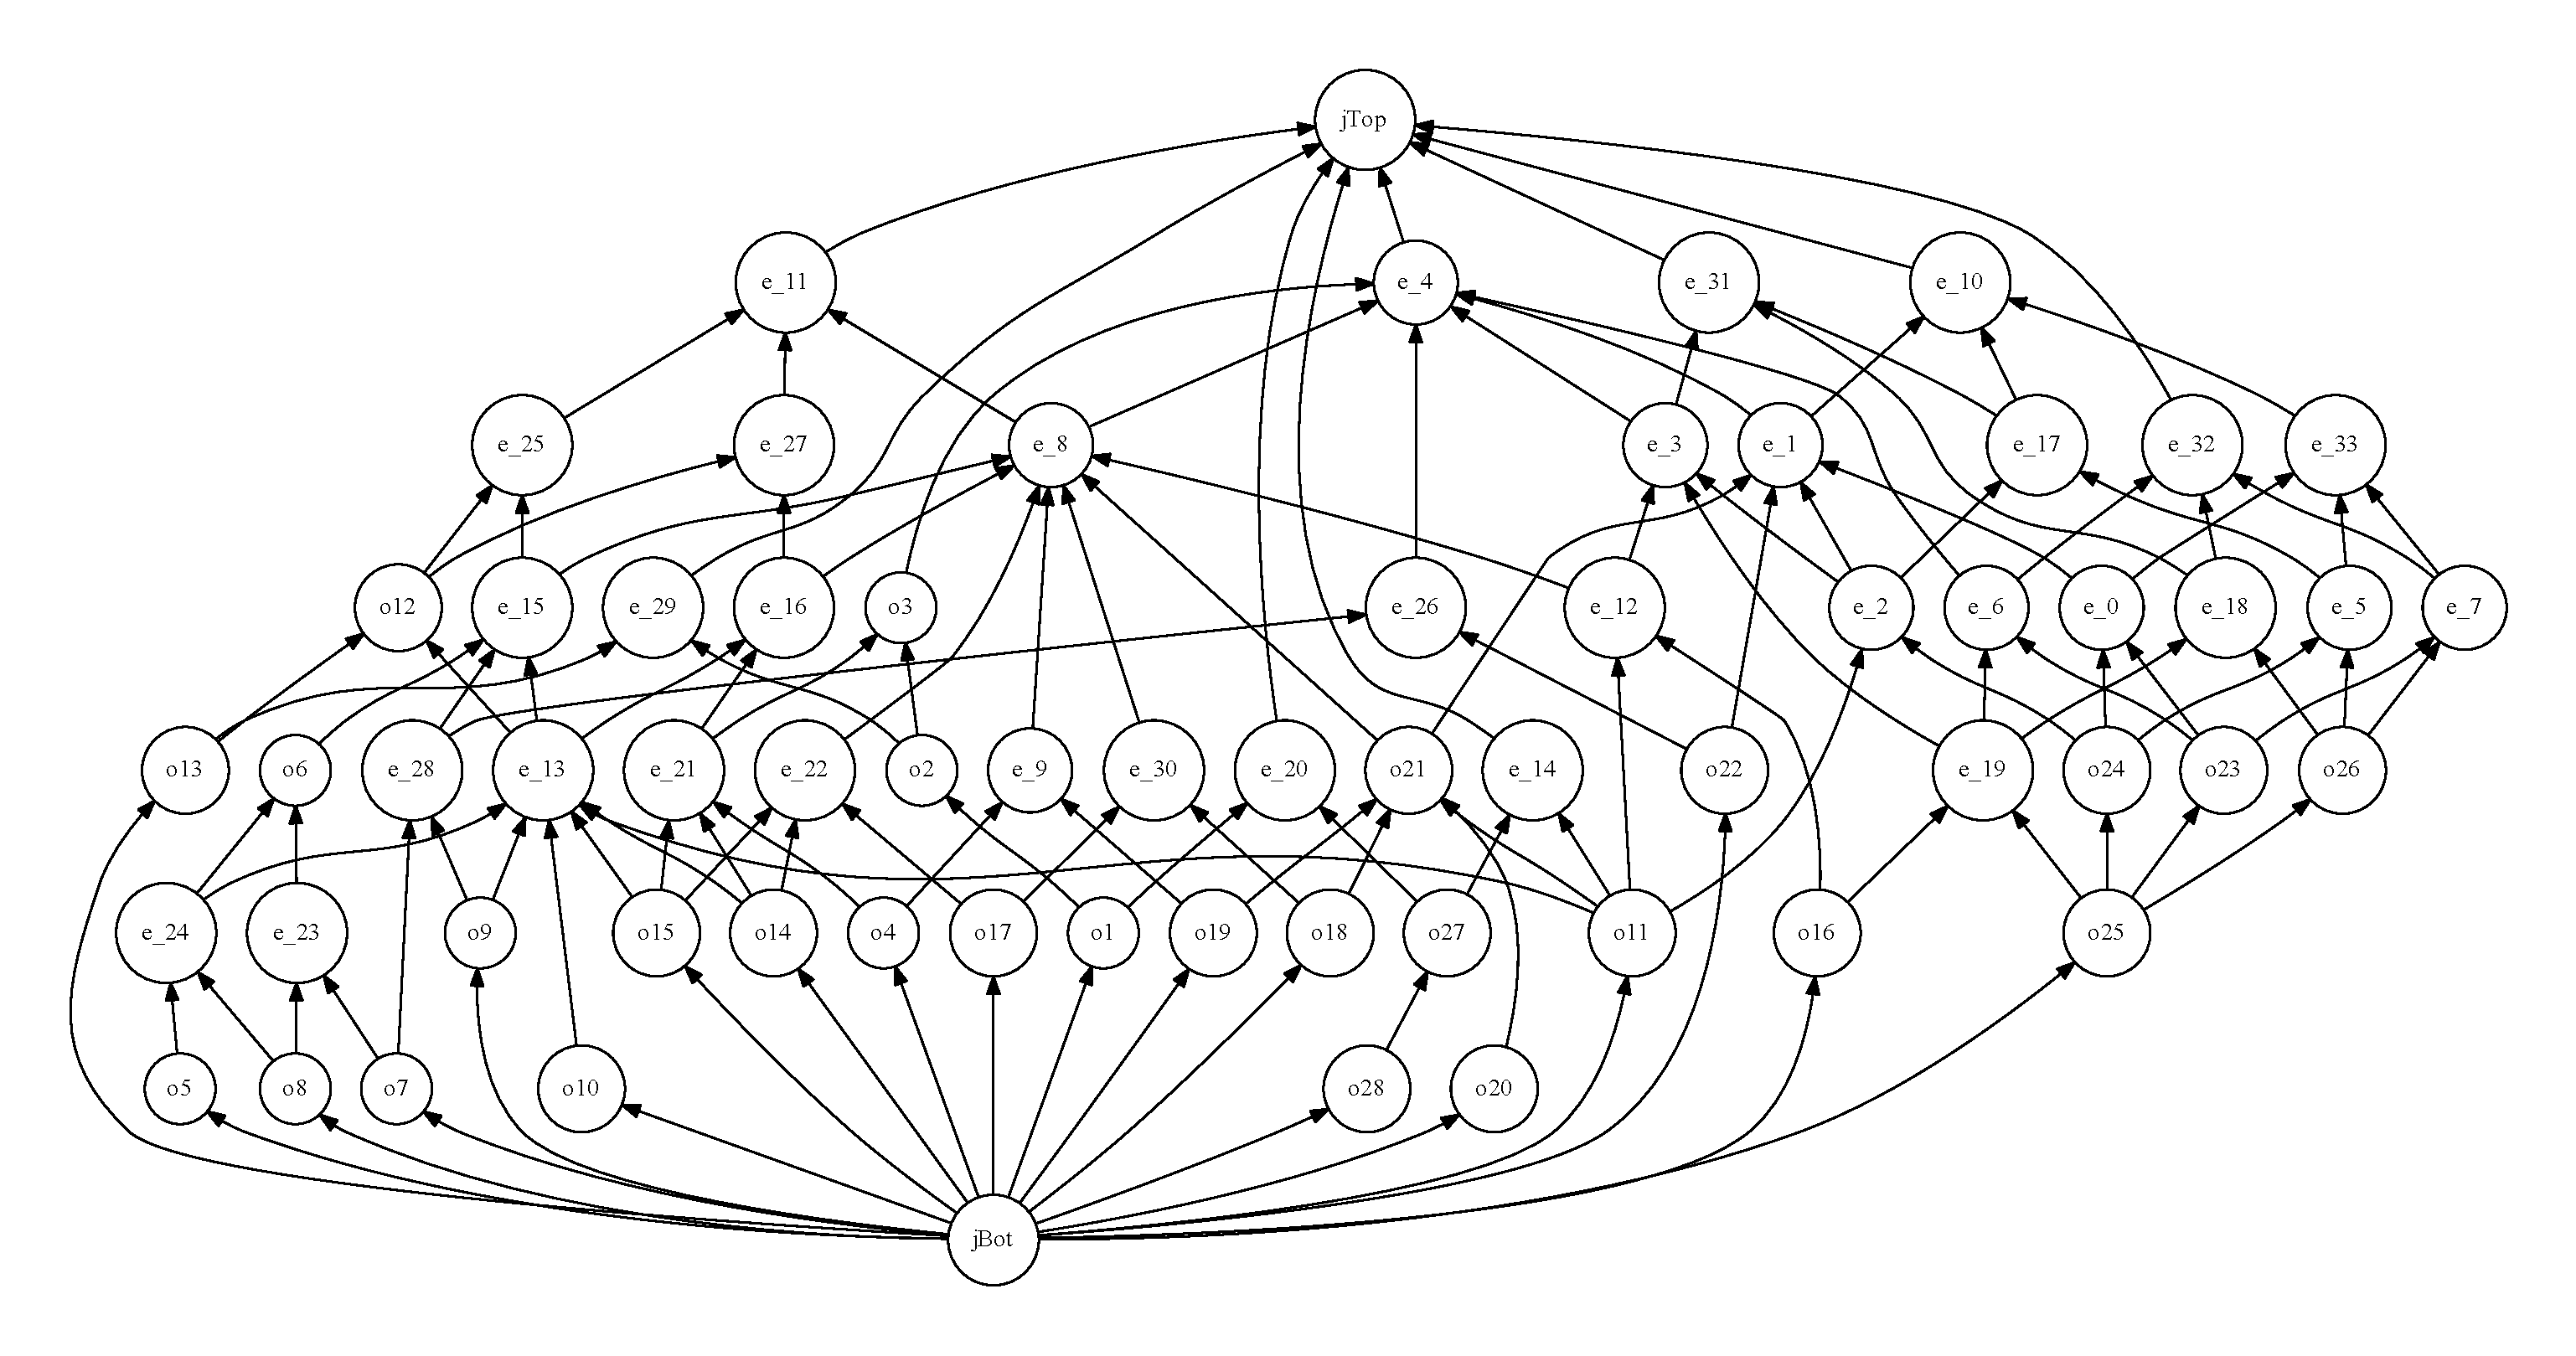
\includegraphics[scale=0.35]{priss2013-table01.pdf}
	\caption{Cas Priss (\cite{MedianConceptLattices})}
\end{figure}

\chapter{Fichiers d'entré et de sortie}
\label{inputoutput}

Cette annexe présente le fichier texte d'entré contenant le contexte de base et le fichier texte de sortie pour l'utilisation du résultat sous ConExp.

\subsection*{Input}

Le fichier d'entré peut prendre de multiples formes. Il demande néanmoins d'avoir en première ligne les attributs séparé par une tabulation. Chaque ligne suivant correspondra à un nouvel objet sans avoir à indiquer son labe et dont chaque correspondance ou absence de correspondance séparées par un tabulation. Une non correspondace se marque avec un \guillemotleft{} 0 \guillemotright{} ou l'absence de caractère. La correspondance est signalé par tout autre caractère.

\begin{figure}[H]
	\begin{minipage}[c]{0.5\textwidth}
	\begin{center}
		\begin{tabular}{ c c c c c }
			a1 & a2 & a3 & a4 & a5 \\
			x & x & & x & \\
			 & x & x & & x\\
			x & & & x & \\
			 & & x & & x \\
			 & & & & x \\
		\end{tabular}
	\end{center}
	\end{minipage}
	\begin{minipage}[c]{0.5\textwidth}
	\begin{center}
		\begin{tabular}{ c c c c c }
			a1 & a2 & a3 & a4 & a5 \\
			1 & 1 & 0 & 1 & 0 \\
			0 & 1 & 1 & 0 & 1 \\
			1 & 0 & 0 & 1 & 0 \\
			0 & 0 & 1 & 0 & 1 \\
			0 & 0 & 0 & 1 & 0 \\
			0 & 0 & 0 & 0 & 1 \\
		\end{tabular}
	\end{center}
	\end{minipage}
	\caption{Fichier source de cla\_v1}
\end{figure}

\subsection*{Output}

Le fichier de sortie quant à lui respecte la mise en forme d'importation de ConExp. Les attributs sur la première ligne séparé par une tabulation suivis d'une ligne vide et enfin des correspondances avec un objet par ligne sans indiquer le label et une notation binaire \guillemotleft{} 0 \guillemotright{} et \guillemotleft{} 1 \guillemotright{} indiquant respectivement la non correspondance et la correspondance.

\begin{figure}[H]
	\begin{center}
		\begin{tabular}{ c c c c c }
			a1 & a2 & a3 & a4 & a5 \\
			\\
			1 & 1 & 0 & 1 & 0 \\
			0 & 1 & 1 & 0 & 1 \\
			1 & 0 & 0 & 1 & 0 \\
			0 & 0 & 1 & 0 & 1 \\
			0 & 0 & 0 & 1 & 0 \\
			0 & 0 & 0 & 0 & 1 \\
		\end{tabular}
	\end{center}
	\caption{Exportation de cla\_v1 pour ConExp}
\end{figure}


\end{appendix}

%\part{bloc note}

\section{vrac}

Nous allons prendre en exemple le cas non distributif le plus simple, $N_5$ pour suivre les étapes de l'algorithme \ref{treillis_n5}. Il faut garder à l'esprit de cette méthode vise à obtenir un treillis distributif aussi proche que possible du treillis original.

\begin{figure}[H]
	\begin{center}
		\begin{tikzpicture}
			\node [wnode, label=below:{$\bot$}] (bot) at (0,0) {};
			\node [wnode, label=left:{$1$}] (1) at (-1, 1) {};
			\node [wnode, label=right:{$2$}] (2) at (1, 1) {};
			\node [wnode, label=left:{$3$}] (3) at (-1, 2) {};
			\node [wnode, label={$\top$}] (top) at (0, 3) {};
			
			\path [line] (bot) -- (1);
			\path [line] (bot) -- (2);
			\path [line] (1) -- (3);
			\path [line] (2) -- (top);
			\path [line] (3) -- (top);
		\end{tikzpicture}
	\end{center}
	\caption{Treillis de $N_5$}
	\label{treillis_n5}
\end{figure}

\chapter{Motivations}

\section{ORPAILLEUR}

L'équipe ORPAILLEUR a poursuivi en ce sens \cite{cla2018} en proposant une méthode générale pour générer le graphe médian de façon systèmatique. Nous allons prendre en exemple le cas $N_5$ pour suivre les étapes de l'algorithme. Il faut garder à l'esprit de cette méthode vise à obtenir un treillis distributif aussi proche que possible du treillis original, le tout en garder l'ordre des objets. C'est-à-dire que la relation $o1 < o2$ restera vrai même après la transformation.

\begin{figure}[H]
	\begin{minipage}[c]{0.5\textwidth}
	\begin{center}
		\begin{tabular}{ l | c c c }
			 & A & B & C \\
			\hline
			1 & x & & x \\
			2 & & x & \\
			3 & & & x \\
		\end{tabular}
	\end{center}
	\end{minipage}
	\begin{minipage}[c]{0.5\textwidth}
	\begin{center}
		\begin{tikzpicture}
			\node [wnode, label=below:{bot}] (bot) at (0,0) {};
			\node [bnode, label=left:{1, A}] (1) at (-1, 1) {};
			\node [bnode, label=right:{2, B}] (2) at (1, 1) {};
			\node [bnode, label=left:{3, C}] (3) at (-1, 2) {};
			\node [wnode, label={top}] (top) at (0, 3) {};
			
			\path [line] (bot) -- (1);
			\path [line] (bot) -- (2);
			\path [line] (1) -- (3);
			\path [line] (2) -- (top);
			\path [line] (3) -- (top);
		\end{tikzpicture}
	\end{center}
	\end{minipage}
	\caption{Cas de $N_5$}
\end{figure}

Nous utilisons le contexte réduit de $N_5$. Nous allons créé un nouveau contexte à partir des $\wedge$-irreductibles. Le principe est de tous les parcourir et de crée un attribut pour chacun qui sera en correspondance avec tous les $\wedge$-irreductibles qui ne sont pas dans le filtre de l'attribut en cours.

\begin{figure}[H]
	\begin{minipage}[c]{0.5\textwidth}
	\begin{center}
		\begin{tabular}{ l | c }
			 & m1\\
			\hline
			1 & \\
			2 & x \\
			3 & \\
		\end{tabular}
	\end{center}
	\end{minipage}
	\begin{minipage}[c]{0.5\textwidth}
	\begin{center}
		\begin{tikzpicture}
			\node [wnode, label=below:{bot}] (bot) at (0,0) {};
			\node [bnode, label=left:{1}] (1) at (-1, 1) {};
			\node [bnode, label=right:{2}] (2) at (1, 1) {};
			\node [bnode, label=left:{3}] (3) at (-1, 2) {};
			\node [wnode, label={top}] (top) at (0, 3) {};
			
			\path [line] (bot) -- (1);
			\path [line] (bot) -- (2);
			\path [line] (1) -- (3);
			\path [line] (2) -- (top);
			\path [line] (3) -- (top);
			
			\draw [very thick, dotted] plot [smooth, tension=2] coordinates {(-2.5, 3.5) (-1, 0.5) (0.5, 3.5)};
		\end{tikzpicture}
	\end{center}
	\end{minipage}
	\caption{Étape 1}
\end{figure}

\begin{figure}[H]
	\begin{minipage}[c]{0.5\textwidth}
	\begin{center}
		\begin{tabular}{ l | c c }
			 & m1 & m2\\
			\hline
			1 & & x\\
			2 & x & \\
			3 & & x \\
		\end{tabular}
	\end{center}
	\end{minipage}
	\begin{minipage}[c]{0.5\textwidth}
	\begin{center}
		\begin{tikzpicture}
			\node [wnode, label=below:{bot}] (bot) at (0,0) {};
			\node [bnode, label=left:{1}] (1) at (-1, 1) {};
			\node [bnode, label=right:{2}] (2) at (1, 1) {};
			\node [bnode, label=left:{3}] (3) at (-1, 2) {};
			\node [wnode, label={top}] (top) at (0, 3) {};
			
			\path [line] (bot) -- (1);
			\path [line] (bot) -- (2);
			\path [line] (1) -- (3);
			\path [line] (2) -- (top);
			\path [line] (3) -- (top);
			
			\draw [very thick, dotted] plot [smooth, tension=2] coordinates {(-0.5, 3.5) (1, 0.5) (2.5, 3.5)};
		\end{tikzpicture}
	\end{center}
	\end{minipage}
	\caption{Étape 2}
\end{figure}

\begin{figure}[H]
	\begin{minipage}[c]{0.5\textwidth}
	\begin{center}
		\begin{tabular}{ l | c c c }
			 & m1 & m2 & m3 \\
			\hline
			1 & & x & x \\
			2 & x & & x\\
			3 & & x & \\
		\end{tabular}
	\end{center}
	\end{minipage}
	\begin{minipage}[c]{0.5\textwidth}
	\begin{center}
		\begin{tikzpicture}
			\node [wnode, label=below:{bot}] (bot) at (0,0) {};
			\node [bnode, label=left:{1}] (1) at (-1, 1) {};
			\node [bnode, label=right:{2}] (2) at (1, 1) {};
			\node [bnode, label=left:{3}] (3) at (-1, 2) {};
			\node [wnode, label={top}] (top) at (0, 3) {};
			
			\path [line] (bot) -- (1);
			\path [line] (bot) -- (2);
			\path [line] (1) -- (3);
			\path [line] (2) -- (top);
			\path [line] (3) -- (top);
			
			\draw [very thick, dotted] plot [smooth, tension=2] coordinates {(-2.5, 3.5) (-1, 1.5) (0.5, 3.5)};
		\end{tikzpicture}
	\end{center}
	\end{minipage}
	\caption{Étape 3}
\end{figure}

Uns fois ce nouveau contexte optenu, il suffit de tracer le treillis associé.

\begin{figure}[H]
	\begin{minipage}[c]{0.5\textwidth}
	\begin{center}
		\begin{tabular}{ l | c c c }
			 & m1 & m2 & m3 \\
			\hline
			1 & & x & x \\
			2 & x & & x\\
			3 & & x & \\
		\end{tabular}
	\end{center}
	\end{minipage}
	\begin{minipage}[c]{0.5\textwidth}
	\begin{center}
		\begin{tikzpicture}
			\node [wnode, label=below:{bot}] (bot) at (0,0) {};
			\node [wnode, label=left:{1}] (1) at (-1, 1) {};
			\node [wnode, label=right:{2, m1}] (2) at (1, 1) {};
			\node [wnode, label=left:{3, m2}] (3) at (-1, 2) {};
			\node [bnode, label=right:{m3}] (4) at (1, 2) {};
			\node [wnode, label={top}] (top) at (0, 3) {};
			
			\path [line] (bot) -- (1);
			\path [line] (bot) -- (2);
			\path [line] (1) -- (3);
			\path [line] (1) -- (4);
			\path [line] (2) -- (4);
			\path [line] (3) -- (top);
			\path [line] (4) -- (top);
		\end{tikzpicture}
	\end{center}
	\end{minipage}
	\caption{$N_5$ après transformation}
\end{figure}

Nous obtenons ainsi un nouveau contexte pour un nouveau treillis distributif très proche du treillis de base. Mais cela reste que la première étape de la proposition de Utas Priss. Il faut à présent appliquer cette méthode dans le cas complet. Nous prendrons deux exemples, le premier fonctionne correctement et est basé sur l'exemple précédent ($N_5$) et le second va permettre de mettre en évidence le problème qui est à la source de mon travail. Nous appellerons cette méthode globale, la \guillemotleft{} méthode cla \guillemotright{}.

\begin{figure}[H]
	\begin{minipage}[c]{0.5\textwidth}
	\begin{center}
		\begin{tabular}{ l | c c c c c c }
			 & A & B & C & D & E & F \\
			\hline
			1 & x & x & x & & & \\
			2 & x & & x & & & \\
			3 & & x & & & & \\
			4 & & & x & & & \\
			5 & & & & x & x & x \\
			6 & & & & x & & x \\
			7 & & & & & x & \\
			8 & & & & & & x \\
		\end{tabular}
	\end{center}
	\end{minipage}
	\begin{minipage}[c]{0.5\textwidth}
	\begin{center}
		\begin{tikzpicture}
			\node [wnode, label=below:{bot}] (bot) at (0,0) {};
			\node [bnode, label=left:{1}] (1) at (-2, 1) {};
			\node [bnode, label=right:{5}] (5) at (2, 1) {};
			
			\node [bnode, label=left:{2, A}] (2) at (-3, 2) {};
			\node [bnode, label=right:{3, B}] (3) at (-1, 2) {};
			\node [bnode, label=left:{4, C}] (4) at (-3, 3) {};
			
			\node [bnode, label=right:{6, D}] (6) at (3, 2) {};
			\node [bnode, label=right:{7, E}] (7) at (1, 2) {};
			\node [bnode, label=right:{8, F}] (8) at (3, 3) {};
			
			\node [wnode, label={top}] (top) at (0, 4) {};
			
			\path [line] (bot) -- (1);
			\path [line] (bot) -- (5);
			
			\path [line] (1) -- (2);
			\path [line] (1) -- (3);
			\path [line] (2) -- (4);
			\path [line] (3) -- (top);
			\path [line] (4) -- (top);
			
			\path [line] (5) -- (6);
			\path [line] (5) -- (7);
			\path [line] (6) -- (8);
			\path [line] (7) -- (top);
			\path [line] (8) -- (top);
		\end{tikzpicture}
	\end{center}
	\end{minipage}
	\caption{Cas fonctionnel, état de départ}
\end{figure}

À partir de là, on extrait chaque contexte des atomes pour les traiter suivant l'algorithme vu précédamment.

\begin{figure}[H]
	\begin{minipage}[c]{0.5\textwidth}
	\begin{center}
		\begin{tabular}{ l | c c c }
			C1 & A & B & C \\
			\hline
			2 & x & & x \\
			3 & & x & \\
			4 & & & x \\
		\end{tabular}
	\end{center}
	\end{minipage}
	\begin{minipage}[c]{0.5\textwidth}
	\begin{center}
		\begin{tabular}{ l | c c c }
			C1 & m2 & m3 & m4 \\
			\hline
			2 & & x & x \\
			3 & x & & x \\
			4 & & x & \\
		\end{tabular}
	\end{center}
	\end{minipage}
	\caption{Cas fonctionnel, contexte atome 1}
\end{figure}

\begin{figure}[H]
	\begin{minipage}[c]{0.5\textwidth}
	\begin{center}
		\begin{tabular}{ l | c c c }
			C2 & D & E & F \\
			\hline
			6 & x & & x \\
			7 & & x & \\
			8 & & & x \\
		\end{tabular}
	\end{center}
	\end{minipage}
	\begin{minipage}[c]{0.5\textwidth}
	\begin{center}
		\begin{tabular}{ l | c c c }
			C2 & m6 & m7 & m8 \\
			\hline
			6 & & x & x \\
			7 & x & & x \\
			8 & & x & \\
		\end{tabular}
	\end{center}
	\end{minipage}
	\caption{Cas fonctionnel, contexte atome 2}
\end{figure}

Puis pour la mise en commun on assemble tout simplement les contextes obtenus sans oublié d'ajouter les atomes et leur correspondance avec les attributs de leur contexte respectif.

\begin{figure}[H]
	\begin{minipage}[c]{0.5\textwidth}
	\begin{center}
		\begin{tabular}{ l | c c c c c c }
			 & m2 & m3 & m4 & m6 & m7 & m8 \\
			\hline
			1 & x & x & x & & & \\
			2 & & x & x & & & \\
			3 & x & & x & & & \\
			4 & & x & & & & \\
			5 & & & & x & x & x \\
			6 & & & & & x & x \\
			7 & & & & x & & x \\
			8 & & & & & x & \\
		\end{tabular}
	\end{center}
	\end{minipage}
	\begin{minipage}[c]{0.5\textwidth}
	\begin{center}
		\begin{tikzpicture}
			\node [wnode, label=below:{bot}] (bot) at (0,0) {};
			\node [wnode, label=left:{1}] (1) at (-2, 1) {};
			\node [wnode, label=right:{5}] (5) at (2, 1) {};
			
			\node [wnode, label=left:{2}] (2) at (-3, 2) {};
			\node [wnode, label=right:{3, m2}] (3) at (-1, 2) {};
			\node [wnode, label=left:{4, m3}] (4) at (-3, 3) {};
			\node [bnode, label=left:{m4}] (m4) at (-1, 3) {};
			
			\node [wnode, label=right:{6}] (6) at (3, 2) {};
			\node [wnode, label=right:{7, m6}] (7) at (1, 2) {};
			\node [wnode, label=right:{8, m7}] (8) at (3, 3) {};
			\node [bnode, label=right:{m8}] (m8) at (1, 3) {};
			
			\node [wnode, label={top}] (top) at (0, 4) {};
			
			\path [line] (bot) -- (1);
			\path [line] (bot) -- (5);
			
			\path [line] (1) -- (2);
			\path [line] (1) -- (3);
			\path [line] (2) -- (4);
			\path [line] (2) -- (m4);
			\path [line] (3) -- (m4);
			\path [line] (4) -- (top);
			\path [line] (m4) -- (top);
			
			\path [line] (5) -- (6);
			\path [line] (5) -- (7);
			\path [line] (6) -- (8);
			\path [line] (6) -- (m8);
			\path [line] (7) -- (m8);
			\path [line] (8) -- (top);
			\path [line] (m8) -- (top);
		\end{tikzpicture}
	\end{center}
	\end{minipage}
	\caption{Cas fonctionnel, état final}
\end{figure}

Comme nous pouvons le voir, tout se déroule comme prévu, tous les treillis des atomes sont devenus distributifs et le treillsi général reste très proche du treillis d'origine. Nous sommes arrivé à l'objectif désiré. Maintenant voyons voir ce qu'il peut se passer lorsqu'un concept est commun à plusieurs atomes. C'est un cas choisi délibérément parce qu'il pose problème, tous les concepts qui sont commun à plusieurs atomes ne posent pas forcement problème mais c'est une condition pour qu'il le soit. Nous appellerons ce cas, le \guillemotleft{} cas cla \guillemotright{}.

\begin{figure}[H]
	\begin{minipage}[c]{0.5\textwidth}
	\begin{center}
		\begin{tabular}{ l | c c c c c }
			 & A & B & C & D & E \\
			\hline
			1 & x & x & x & & \\
			2 & x & x & & & \\
			3 & & x & & & \\
			4 & & & x & x & x \\
			5 & & & & x & x \\
			5 & & & & & x \\
		\end{tabular}
	\end{center}
	\end{minipage}
	\begin{minipage}[c]{0.5\textwidth}
	\begin{center}
		\begin{tikzpicture}
			\node [wnode, label=below:{bot}] (bot) at (0,0) {};
			\node [wnode, label=left:{1}] (1) at (-1, 1) {};
			\node [wnode, label=right:{4}] (4) at (1, 1) {};
			
			\node [wnode, label=left:{2, A}] (2) at (-2, 2) {};
			\node [wnode, label=left:{3, B}] (3) at (-2, 3) {};
			
			\node [wnode, label=right:{5, D}] (5) at (2, 2) {};
			\node [wnode, label=right:{6, E}] (6) at (2, 3) {};
			
			\node [bnode, label=right:{C}] (C) at (0, 2) {};
			
			\node [wnode, label={top}] (top) at (0, 4) {};
			
			\path [line] (bot) -- (1);
			\path [line] (bot) -- (4);
			
			\path [line] (1) -- (2);
			\path [line] (1) -- (C);
			\path [line] (2) -- (3);
			\path [line] (3) -- (top);
			
			\path [line] (4) -- (5);
			\path [line] (4) -- (C);
			\path [line] (5) -- (6);
			\path [line] (6) -- (top);
			
			\path [line] (C) -- (top);
		\end{tikzpicture}
	\end{center}
	\end{minipage}
	\caption{Cas non fonctionnel, état de départ}
\end{figure}

On refait les mêmes étapes de précédemment, extraction des contextes des atomes et application de l'algorithme puis remise en commun.

\begin{figure}[H]
	\begin{minipage}[c]{0.5\textwidth}
	\begin{center}
		\begin{tabular}{ l | c c c c c c }
			 & m1 & m2 & m3 & m4 & m5 & m6 \\
			\hline
			1 & & x & x & x & x & x \\
			2 & & & x & x & & \\
			3 & & & & x & & \\
			4 & x & x & x & & x & x \\
			5 & x & & & & & x \\
			6 & x & & & & & \\
		\end{tabular}
	\end{center}
	\end{minipage}
	\begin{minipage}[c]{0.5\textwidth}
	\begin{center}
		\begin{tikzpicture}
			\node [wnode, label=below:{bot}] (bot) at (0,0) {};
			\node [wnode, label=left:{1}] (1) at (-1, 1) {};
			\node [bnode, label=right:{4}] (4) at (1, 1) {};
			
			\node [wnode, label=left:{2}] (2) at (-2, 2) {};
			\node [wnode, label=left:{3, m4}] (3) at (-2, 3) {};
			
			\node [bnode, label=right:{5}] (5) at (2, 2) {};
			\node [wnode, label=right:{6, m1}] (6) at (2, 3) {};
			
			\node [bnode, label=right:{m2, m5}] (m2) at (0, 2) {};
			\node [bnode, label=left:{m3}] (m3) at (-0.5, 3) {};
			\node [wnode, label=right:{m6}] (m6) at (0.5, 3) {};
			
			\node [bnode, label={top}] (top) at (0, 4) {};
			
			\path [line] (bot) -- (1);
			\path [line] (bot) -- (4);
			
			\path [line] (1) -- (2);
			\path [line] (1) -- (m2);
			\path [line] (2) -- (3);
			\path [line] (3) -- (top);
			
			\path [line] (4) -- (5);
			\path [line] (4) -- (m2);
			\path [line] (5) -- (6);
			\path [line] (6) -- (top);
			
			\path [line] (m2) -- (m3);
			\path [line] (m2) -- (m6);
			\path [line] (m3) -- (top);
			\path [line] (m6) -- (top);
			
			\path [line] (2) -- (m3);
			\path [line] (5) -- (m6);
		\end{tikzpicture}
	\end{center}
	\end{minipage}
	\caption{Cas non fonctionnel, état final}
\end{figure}

Nous pouvons voir que les n\oe uds m3 et m6 posent problème. m3 qui a été ajouté par l'algorithme appliqué au contexte de l'atome 1 provoque la création d'un nouveau treillis $N_5$ dans le treillis de l'atome 4, le rendant de ce fait non distributif. L'idéal désiré serait un treillis où les n\oe uds m3 et m6 ne font qu'un.

\begin{figure}[H]
	\begin{center}
		\begin{tikzpicture}
			\node [wnode, label=below:{bot}] (bot) at (0,0) {};
			\node [wnode, label=left:{1}] (1) at (-1, 1) {};
			\node [wnode, label=right:{4}] (4) at (1, 1) {};
			
			\node [wnode, label=left:{2}] (2) at (-2, 2) {};
			\node [wnode, label=left:{3, m4}] (3) at (-2, 3) {};
			
			\node [wnode, label=right:{5}] (5) at (2, 2) {};
			\node [wnode, label=right:{6, m1}] (6) at (2, 3) {};
			
			\node [wnode, label=right:{m2, m5}] (m2) at (0, 2) {};
			\node [bnode, label=right:{m3, m6}] (m3) at (0, 3) {};
			
			\node [wnode, label={top}] (top) at (0, 4) {};
			
			\path [line] (bot) -- (1);
			\path [line] (bot) -- (4);
			
			\path [line] (1) -- (2);
			\path [line] (1) -- (m2);
			\path [line] (2) -- (3);
			\path [line] (3) -- (top);
			
			\path [line] (4) -- (5);
			\path [line] (4) -- (m2);
			\path [line] (5) -- (6);
			\path [line] (6) -- (top);
			
			\path [line] (m2) -- (m3);
			\path [line] (m3) -- (top);
			
			\path [line] (2) -- (m3);
			\path [line] (5) -- (m3);
		\end{tikzpicture}
	\end{center}
	\caption{Cas non fonctionnel, état final désiré}
\end{figure}

\chapter{Définitions}

\section*{Généralité}

On dispose d'un ensemble d'objets noté $J$ et d'un ensemble de propriétés noté $M$, le tout représenté dans un contexte $C$ (figure \ref{contexte_fca}) où chaque objet est en concordance avec les attributs qu'il possède, cet ensemble est noté $I$. Un contexte est noté $C(J, M, I)$. On peut également utiliser un treillis (figure \ref{treillis_fca})pour une représentation plus visuelle.

\begin{figure}[H]
	\begin{minipage}{0.4\textwidth}
	\begin{center}
		\begin{tabular}{ l | c c c }
			 & A: poisson & B: oiseau & C: ovipare \\
			\hline
			1: poisson rouge & x &  & x \\
			2: chevalier gambette &  & x & x \\
			3: guppy & x &  &  \\
		\end{tabular}
		\caption{Contexte}
		\label{contexte_fca}
	\end{center}
	\end{minipage}
	\begin{minipage}{0.8\textwidth}
	\begin{center}
		\begin{tikzpicture}
			\node [bnode, label=below:{bot}] (bot) at (0,0) {};
			\node [bnode, label=left:{1}] (1) at (-1, 1) {};
			\node [bnode, label=right:{2, B}] (2) at (1, 1) {};
			\node [bnode, label=left:{3, A}] (3) at (-1, 2) {};
			\node [bnode, label=right:{C}] (4) at (1, 2) {};
			\node [bnode, label={top}] (top) at (0, 3) {};
			
			\path [line] (bot) -- (1);
			\path [line] (bot) -- (2);
			\path [line] (1) -- (3);
			\path [line] (1) -- (4);
			\path [line] (2) -- (4);
			\path [line] (3) -- (top);
			\path [line] (4) -- (top);
		\end{tikzpicture}
	\end{center}
	\caption{Treillis}
	\label{treillis_fca}
	\end{minipage}
\end{figure}

On dispose également d'un vocabulaire propre au domaine pour faciliter les échanges.\\
Un concept peut être vu comme un n\oe ud du treillis, il correspond à un ensemble d'objets et d'attributs. Par exemple le n\oe ud avec le label \guillemotleft{} poisson rouge \guillemotright{} correpond à l'ensemble d'objets \{1\} et à l'ensemble d'attributs \{A, C\}. Afin de faciliter la communication il est commun d'utiliser l'objet ou l'attribut lorsqu'ils sont uniques, pour parler d'un concept, on parlera donc du concept 1 ou du concept poisson rouge. Le filtre d'un concept est l'ensemble des concepts qui y sont contenu et est noté : $\uparrow \! 1 = \{1, 3\}$. À l'inverse, l'idéal d'un concept est l'ensemble des concepts qui le contiennent et est noté : $\downarrow \! 3 = \{1, 3\}$. Un opérateur \guillemotleft{} ` \guillemotright{} est aussi utilisé. Il permet de faire la transition entre un objet et ses attributs : $3'' = \{A\}' = \{1, 3\}$ ou entre un attribut et ses objets : $A'' = \{1, 3\}' = \{A\}$. On appelle infimum de plusieurs concepts celui qui est à l'intersetion des attributs de ceux-ci, noté $\wedge$ tel que $A \wedge C = 1$. Si un concept est l'infimum (inf) de tous les autres concepts, alors il est le \guillemotleft{} bot \guillemotright{}. À l'inverse, on appelle supremum (sup) de plusieurs concepts celui qui est à l'intersection des objets de ceux-ci, noté $\vee$ tel que $1 \vee 2 = C$. Si un concept est le supremum de tous les autres concepts, alors il est le \guillemotleft{} top \guillemotright{}. Nous définissons également les infimums irréductibles, $\wedge$-irréductibles, (resp. supremums irréductibles, $\vee$-irréductibles) les concepts ayant au plus un unique inf direct (resp. sup direct). Ce sont les concepts qu'on retrouve dans le contexte réduit. Nous définissons comme atomes les concepts supremum direct du bot, dans la figure 2.2 cela correpondrait aux concepts 1, et 2.

\bigbreak

Il existe plusieurs catégories de contexte.\\
Tout d'abord nous avons le contexte quelconque (figure \ref{contexte_quelconque}), il ne dispose d'aucunes règles ni propriétés en plus de la base développée dans la section précédente. Puis nous avons le contexte clarifié (figure \ref{contexte_clarifié}), dans celui-ci nous ne voulons aucun doublon de données. Si nous avons deux objets (resp. attributs) ayant exactement les mêmes concordances avec les attributs (resp. objets) alors on en supprime un de la table. Enfin le contexte réduit (figure \ref{contexte_réduit}), il est la version la plus petite sans perte de données. On supprime de la table tous les objets (resp. attribut) qui sont obtenable par l'intersection d'une combinaison des autres objets (resp. attributs). C'est cette version du contexte qui est communément utilisé.

\begin{figure}[H]
	\begin{minipage}[t]{0.3\textwidth}
	\begin{center}
		\begin{tabular}{ l | c c c c }
			 & A & B & C \\
			\hline
			1 & x &  & x \\
			2 &  & x & x \\
			3 &  & x & x \\
			4 & x &  &  \\
			5 &  &  & x \\
		\end{tabular}
		\caption{Contexte quelconque}
		\label{contexte_quelconque}
	\end{center}
	\end{minipage}
	\begin{minipage}[t]{0.3\textwidth}
	\begin{center}
		\begin{tabular}{ l | c c c c }
			 & A & B & C \\
			\hline
			1 & x &  & x \\
			2 &  & x & x \\
			4 & x &  &  \\
			5 &  &  & x \\
		\end{tabular}
		\caption{Contexte clarifié}
		\label{contexte_clarifié}
	\end{center}
	\end{minipage}
	\begin{minipage}[t]{0.3\textwidth}
	\begin{center}
		\begin{tabular}{ l | c c c c }
			 & A & B & C \\
			\hline
			1 & x &  & x \\
			2 &  & x & x \\
			4 & x &  &  \\
		\end{tabular}
		\caption{Contexte réduit}
		\label{contexte_réduit}
	\end{center}
	\end{minipage}
\end{figure}

\section{Algorithme de cla}

\begin{figure}[H]
\begin{algorithm}[H]
	\DontPrintSemicolon
	\caption{Construction de contexte de treillis distributif}

	\KwData{Context réduit $C(J, M, \leq_{C})$}
	\KwResult{Contexte réduit $C_d(J, M_d, I_d)$ de $(\mathcal{O}(J), \subseteq, \cap, \cup)$}

	\Begin{
		$M_d \leftarrow \emptyset$\;
		$I_d \leftarrow \emptyset$\;
		\ForEach{$j \in J$}{
			$\uparrow j \leftarrow \emptyset$\;
			\ForEach{$i \in J$}{
				\If{$j' \subseteq i'$}{
					$\uparrow j \leftarrow \uparrow j \cup i$\;
				}
			}
			$M_d \leftarrow M_d \cup m_j$\;
			$X \leftarrow J \setminus \uparrow j$\;
			\ForEach{$x \in X$}{
				$I_d \leftarrow I_d \cup (x, m_j)$\;
			}
		}
	}
\end{algorithm}
\caption{Construction de contexte de treillis distributif}
\label{algo_cla}
\end{figure}

\end{document}